\documentclass[electronic]{kthesis}

%%%%%%%%%%%%%%%%%
%%%% PACKAGES %%%
%%%%%%%%%%%%%%%%%
\usepackage[utf8x]{inputenc}
\usepackage[swedish,english]{babel}
\usepackage{enumerate}  % for capital latin numbers in the list of papers
\usepackage{caption}   % to align the table caption to the right/left
\usepackage{lscape}
\usepackage{hyperref}  %for references
\usepackage{amsmath,mathrsfs}
\usepackage{amssymb}  % assumes amsmath package installed
\usepackage{epstopdf}
\usepackage{subfig}
\usepackage{cite}
\usepackage{graphicx}
\usepackage{bm}	%Command \bm{make bold}
\usepackage{algorithm}
\usepackage{algpseudocode}
\usepackage{algpascal}
\usepackage{multicol}
\usepackage[x11names]{xcolor}
\usepackage{lipsum}

% my packages
\usepackage{comment}

\hypersetup{
	colorlinks = true,
	citecolor = {blue},
	%menubordercolor = {blue},
	%linkbordercolor = {blue},
}

\usepackage{tikz}
\usetikzlibrary{tikzmark,calc,decorations.pathreplacing}
\newcommand{\Depth}{2}
\newcommand{\Height}{2}
\newcommand{\Width}{2}

\renewcommand{\labelitemi}{\textcolor{IndianRed3}{\bfseries\textbullet}}


%%%%%%%%%%%%%%%%%%%%%%%%%%%%%%%%%%%%%%%
%%%%%%%%% Document starts here %%%%%%%%
%%%%%%%%%%%%%%%%%%%%%%%%%%%%%%%%%%%%%%%
\begin{document}
	
%%%%%%%%%%%%%%%%%%%%%%%%%%%%%%%%%%%%%%%%%%
%%%%%% First and second pages %%%%%%%%%%%%
%%%%%%%%%%%%%%%%%%%%%%%%%%%%%%%%%%%%%%%%%%
\title{ Thesis Title }
\subtitle{\textbf{sub-title}}
\author{Marcus Klasson}
\date{date}
\thesistype{Doctoral Thesis}
\imprint{Stockholm, Sweden, 2020}
\examen{Teknologie doktorexamen i elektroteknik}
\disputationsdatum{fredagen den 18 januari 2020 klockan 14.00}
\disputationslokal{Sal F3, Lindstedtsvägen 26, Kungliga Tekniska H\"{o}gskolan, Stockholm}
\publisher{Universitetsservice US AB}
\address{KTH Royal Institute of Technology \\School of Electrical Engineering and Computer Science\\ Division of Fusion Plasma Physics \\ SE-10044 Stockholm\\ Sweden}
\isbn{ISBN 100-}
%\issn{ISSN XXX} % No longer used at KTH
\trita{TRITA-EECS-AVL-2020:4}
\kthlogo{KTHLogo}
	
% Create title page using info above
\maketitle

\frontmatter % Pages i, ii, iii, iv, v etc.
%%%%%%%%%%%%%%%%%%%%%%%%%%%%%%%%%%%
%%%%%%%%%%% ABSTRACT %%%%%%%%%%%%%%
%%%%%%%%%%%%%%%%%%%%%%%%%%%%%%%%%%%
\begin{abstract}

\noindent In recent years, computer vision-based assistive technologies have enabled visually impaired people to use automatic visual recognition on their mobile phones. 
These systems should be capable of recognizing objects on fine-grained levels to provide the user with accurate predictions. Additionally, the user should have the option to update the system continuously to recognize new objects of interest. 
However, there are several challenges that need to be tackled to enable such features with assistive vision systems in real and highly-varying environments. 
For instance, fine-grained image recognition usually requires large amounts of labeled data to be robust. %, and
Moreover, image classifiers struggle with retaining performance of previously learned abilities when they are adapted %adapting 
to new tasks. 
This thesis is divided into two parts where we address these challenges. 
First, we focus on the application of using assistive vision systems for grocery shopping, where items are naturally structured based on fine-grained details.  
We demonstrate how image classifiers can be trained with a combination of natural images and web-scraped information about the groceries to obtain more accurate classification performance compared to only using natural images for training. 
Thereafter, we bring forward a new approach for continual learning called replay scheduling, where we select which tasks to replay at different times to improve memory retention. 
Furthermore, we propose a novel framework for learning replay scheduling policies that can generalize to new continual learning scenarios for mitigating the catastrophic forgetting effect in image classifiers. 
This thesis provides insights on practical challenges that need to be addressed to enhance the usefulness of computer vision for assisting the visually impaired in real-world scenarios. 

\begin{comment}
\noindent In recent years, computer vision-based assistive technologies have enabled visually impaired people to use automatic visual recognition on their mobile phones. 
These systems should be capable of recognizing objects on fine-grained levels to provide the user with accurate predictions. Additionally, the user should have the option to update the system continuously to recognize new objects of interest.  %Moreover, a valuable feature would be if they could be updated to recognize new object classes. 
However, there are several challenges that need to be tackled to enable such features with assistive vision systems in real and highly-varying environments. 
For instance, fine-grained image recognition usually requires large amounts of labeled data to be robust, and image classifiers struggle with retaining performance of previously learned abilities when adapting to new tasks. 
This thesis is divided into two parts where we address these challenges. 
First, we focus on the application of using assistive vision devices for grocery shopping where items are naturally structured based on fine-grained details.  %grocery shopping with an assistive vision device where items are naturally structured based on fine-grained details. 
We demonstrate how image classifiers can be trained with a combination of natural images and web-scraped information about the groceries to obtain more accurate classification performance compared to only using natural images for training. %To reduce the need for exhaustive data collection in grocery stores, we show how image classifiers can be trained with a combination of real images and web-scraped information about the groceries to obtain more accurate classification performance.
Secondly, we bring forward a new approach for continual learning called replay scheduling where we select which tasks to replay at different times to improve memory retention. 
Furthermore, we propose a novel framework for learning replay scheduling policies that can generalize to new continual learning scenarios for mitigating the catastrophic forgetting effect in image classifiers. 
This %To summarize, this 
thesis provides insights on practical challenges that need to be addressed to enhance the usefulness of computer vision for assisting the visually impaired in real-world scenarios. 
\end{comment}



%To address these challenges, 

%Problems with fine-grained image recognition is that it requires large amounts of training data for being robust in real environments with high-variations. 

%The problem with updating the object recognizer continuously is that the recognizer typically suffers from catastrophic forgetting, such that it is hard to guarantee that the recognizer will accurately recognize previously learned objects after learning new ones. 

%This thesis has been divided into two parts targeting these challenges. For fine-grained recognition, we focus on the application of grocery shopping with an assistive vision device. To reduce the need for exhaustive data collection in grocery stores, we show how image classifiers can be trained with a combination of real images and web-scraped information about the groceries to obtain more accurate classification performance. 

%In continual learning, we bring forward a new approach called replay scheduling where we select which tasks to replay at different times. Moreover, we propose a framework for learning replay scheduling policies that can generalize to new continual learning scenarios for mitigating catastrophic forgetting. 


%This thesis provides approaches motivated from real-world applications as well as insights towards automatic visual recognition to assist the visually impaired. 

%To tackle the challenges with fine-grained image recognition, we propose combining learning from web information to reduce the need for collecting real-world images. We have collected a dataset of grocery items in addition to web-scraped information of the items and suggest a method based on multi-view representation learning that enhances the classification performance when combing learning fro real images and web information over learning from only real images. 

%To tackle the catastrohic forgetting, we propose a novel approach called repla yscheduling for mititgating catastrophic forgetting where we select which old tasks to rehearse on at differetn times. We show that repla yscheduling is important in continual learning settings as well as propose a method to enable more efficient scheduling policies that can generalzie to new scenarios without added training cost. 

%Why is this work imporatnt for assistive vision?


%These systems should be capable of recognizing objects that are important for the user on a fine-grained level. To this end, we have focused on the particular application of classifying food items which can be challenging for blind/low-vision people since visual information is often required for distinguishing between similar items. In Paper A, we present a challenging image dataset of groceries taken in grocery stores where each item is hierarchically labeled to capture the fine-grained structure of the various items. Furthermore, we demonstrate in Paper B how more easily accessible information about the items, such as web-scraped images and text descriptions, can be utilized for enhancing the classification performance of groceries compared to only using the real-world images for training. 

%A valuable feature of assistive vision systems is the capability of adapting to new object classes. The main challenge here is to avoid catastrophically forgetting previously learned knowledge when the classifier is updated with new classes. In Paper C, we propose a new continual learning setting for replay-based methods that aligns well with real-world needs where constraints are placed on processing time rather than the storage capacity of old samples. 
%Replay methods mitigate this problem efficiently by mixing previous data samples from a limited memory buffer with the training samples of the new classes during learning. In Paper C, we propose a new continual learning setting that is close to real-world needs where constraints are placed on processing time rather than the storage capacity of old samples. 
%We then study the timing of replaying certain tasks and show that learning replay schedules over which tasks to replay can be critical for the final classification performance in our proposed setting. Finally, in Paper D, we present a method based on reinforcement learning for learning a policy for selecting which tasks to replay at different times. The benefit of our learned replay scheduling policy is that it can be applied to any new continual learning scenario for mitigating catastrophic forgetting in a classifier without additional computational cost. 

%To conclude, I will discuss some potential future directions for the development of the next generation of computer vision-based assistive technologies. 
	
\begin{comment}
\noindent In recent years, computer vision-based assistive systems have enabled visually impaired people to use automatic object recognition on their mobile phones. 
These systems should be capable of recognizing objects that are important for the user on a fine-grained level. 
To this end, we have focused on the particular application of classifying food items which can be challenging for blind/low-vision people since visual information is often required for distinguishing between similar items. 
In Paper A, we present a challenging image dataset of groceries taken in grocery stores where each item is hierarchically labeled to capture the fine-grained structure of the various items. 
Furthermore, we demonstrate in Paper B how more easily accessible information about the items, such as web-scraped images and text descriptions, can be utilized for enhancing the classification performance of groceries compared to only using the real-world images for training. 

A valuable feature of assistive vision systems is the capability of adapting to new object classes. 
The main challenge here is to avoid catastrophically forgetting previously learned knowledge when the classifier is updated with new classes. 
In Paper C, we propose a new continual learning setting for replay-based methods that aligns well with real-world needs where constraints are placed on processing time rather than the storage capacity of old samples. 
%Replay methods mitigate this problem efficiently by mixing previous data samples from a limited memory buffer with the training samples of the new classes during learning. In Paper C, we propose a new continual learning setting that is close to real-world needs where constraints are placed on processing time rather than the storage capacity of old samples. 
We then study the timing of replaying certain tasks and show that learning replay schedules over which tasks to replay can be critical for the final classification performance in our proposed setting. 
Finally, in Paper D, we present a method based on reinforcement learning for learning a policy for selecting which tasks to replay at different times. The benefit of our learned replay scheduling policy is that it can be applied to any new continual learning scenario for mitigating catastrophic forgetting in a classifier without additional computational cost. 

To conclude, I will discuss some potential future directions for the development of the next generation of computer vision-based assistive technologies. 
\end{comment}



%which have been mostly ignored in the literature, can have a high influence on the final classification performance. We then propose a new continual learning setting where scheduling over which tasks to replay becomes important 


%, where replay methods common approach to mitigate this problem is by using replay methods which involve mixing a small set of previous data samples with the samples from the new classes to learn during training.

%In the second part of my work, I have focused on continually learning new object classes where the main challenge is to avoid forgetting previously learned knowledge when the classifier is updated with new classes. 

%A common approach to mitigate this problem is by using replay methods which involve mixing a small set of previous data samples with the samples from the new classes to learn during training. However, current replay methods have ignored the time of when to replay certain tasks, which would be essential for fast adaptation in settings where constraints are set on training time rather than storage capacity of old samples. In Paper C, we show that learning the time to learn which tasks to replay can be critical for the CL performance in this setting. 

%In Paper D, we present a method for learning a policy for selecting which tasks to replay at different times with reinforcement learning.      

%Finally, I will discuss future directions and potential research questions for the development of the next generation of computer vision-based assistive technologies. 


\bigskip \bigskip







%50\%:
%The recent advances in computer vision have made it possible to develop vision-based assistive devices to aid visually impaired people with object recognition in different environments. A particular application where assistive vision would be useful is to help the visually impaired with fine-grained classification of food items since visual information is often required to distinguish between similar items. 
%Enabling image classification models to work in this setting requires collecting large amounts of images of food items which is an expensive process in several ways. In the first part of my work, I have shown how more easily accessible information about food items, such as web-scraped images and text descriptions, can be used for enhancing the classification performance of groceries compared to training using natural images only. 

%A valuable feature of assistive vision devices is the capability of adapting to new object classes. The key challenge is to avoid overwriting previous knowledge when the model is updated with new classes, which is called catastrophic forgetting. In the second part of my work, I aim to mitigate this problem using replay methods, which involve mixing previous data samples with incoming samples from new classes during training. 

%Finally, I will discuss a future third part consisting of approaches for scaling replay methods to larger datasets and how to deploy our models in mobile devices.
		
\end{abstract}
	
\bigskip \bigskip \bigskip \bigskip \bigskip
	
%\setlength{\leftskip}{0.3 cm} \textbf {Keywords:} Visual Recognition, Fine-grained Classification, Continual Learning, Visually Impaired People, Assistive Technologies


%%%%%%%%%%%%%%%%%%%%%%%%%%%%%%%%%%%%%%%%
%%%%%%%% SWEDISH ABSTRACT %%%%%%%%%%%%%%
%%%%%%%%%%%%%%%%%%%%%%%%%%%%%%%%%%%%%%%%
\newpage
\selectlanguage{swedish}
\begin{abstract}
\noindent hej
\end{abstract}
\selectlanguage{english}


%%%%%%%%%%%%%%%%%%%%%%%%%%%%%%%%%%%%%%%
%%%%%%% List of papers %%%%%%%%%%%%%%%%
%%%%%%%%%%%%%%%%%%%%%%%%%%%%%%%%%%%%%%%
%*******************************************************************************
%*********************************** List of Papers ****************************
%*******************************************************************************

\chapter{List of Papers}
\label{chap:list_of_papers}

%\let\thefootnote\relax\footnote{Paper I and III are published under license in \textit{Journal of X}}
\begin{enumerate}[A]
	\item \textbf{\textit{A Hierarchical Grocery Store Image Dataset with Visual and Semantic Labels}} \\
	\textbf{Marcus Klasson}, Cheng Zhang, Hedvig Kjellström \\
	In \textit{IEEE Winter Conference on Applications of Computer Vision (2019)}
\end{enumerate}

\begin{enumerate}[B]
	\item \textbf{\textit{Using Variational Multi-view Learning for Classification of Grocery Items}} \\
	\textbf{Marcus Klasson}, Cheng Zhang, Hedvig Kjellström \\
	In \textit{Patterns, Volume 1(8) (2020)}
\end{enumerate}

\begin{enumerate}[C]
	\item \textbf{\textit{Learn the Time to Learn: Replay Scheduling for Continual Learning}} \\
	\textbf{Marcus Klasson}, Hedvig Kjellström, Cheng Zhang \\
	\textit{Under submission}
\end{enumerate}

\begin{enumerate}[D]
	\item \textbf{\textit{Meta Policy Learning for Replay Scheduling in Continual Learning}} \\
	\textbf{Marcus Klasson}, Hedvig Kjellström, Cheng Zhang \\
	\textit{Under preparation}
\end{enumerate}



\begin{comment}
%%%%%%%%%%%%%%%%%%%%%%%% Papers NOT included in THESIS
Other contributions by the author not included in the thesis.
\begin{enumerate}[I]
	\setcounter{enumi}{1}
	\item \textbf{\textit{Title of paper}} \\
	\textbf{First author}, Second author \\
	\textit{Journal (year)}
\end{enumerate}
\end{comment}


%%%%%%%%%%%%%%%%%%%%%%%%%%%%%%%%%%%%%%%
%%%%%%%% ACKNOWLEDGMENT %%%%%%%%%%%%%%%
%%%%%%%%%%%%%%%%%%%%%%%%%%%%%%%%%%%%%%%
%*******************************************************************************
%*********************************** Acknowledgements **************************
%*******************************************************************************

\chapter{Acknowledgements}
\label{chap:acknowledgements}

\noindent hej

%%%%%%%%%%%%%%%%%%%%%%%%%%%%%%%%
%%%%%%%% ACRONYMS %%%%%%%%%%%%%%
%%%%%%%%%%%%%%%%%%%%%%%%%%%%%%%%
%*******************************************************************************
%*********************************** Acronyms **********************************
%*******************************************************************************

\chapter{Acronyms}
\label{chap:acronyms}

List of commonly used acronyms: \\

\begin{tabular}{llll}
	\textbf{AE}		&	Acronym examples \\
	\textbf{CL}		& 	Continual Learning \\
	\textbf{ML}		& 	Machine Learning \\
	\textbf{RL}		& 	Reinforcement Learning \\
	\textbf{VAE}		&	Variational Autoencoder \\
	
\end{tabular}

%% MK: Add List of Figures & Tables

%% MK: Add Summary of Notations

%\input{Content/Dedication}\clearpage
	
\mainmatter % Pages 1, 2, 3...
%%%%%%%%%%%%%%%%%%%%%%%%%%%%%%%%%%%%%%
%%%%%% TABLE OF CONTENTS %%%%%%%%%%%%%
%%%%%%%%%%%%%%%%%%%%%%%%%%%%%%%%%%%%%%
\begingroup
\hypersetup{hidelinks} % to remove hyperlink color on contents
\tableofcontents
\endgroup
%\tableofcontents

%%%%%%%%%%%%%%%%%%%%%%%%%%%%%%%%%%%%%%%%%%%%%%%%%%%%%%
%%%%%%%%%%%%% Main Matter %%%%%%%%%%%%%%%%%%%%%%%%%%%%
%%%%%%%%%%%%%%%%%%%%%%%%%%%%%%%%%%%%%%%%%%%%%%%%%%%%%%

\part{Overview}
%*******************************************************************************
%*********************************** First Chapter *****************************
%*******************************************************************************

\chapter{Introduction}
\label{chap:introduction}

Vision is probably the most important of all senses that humans possess. Our society is built on having this ability. For example, if we would like to cross a street, there are thick colored stripes on the road or signs above head height that indicate where the cross walk is located such that we can cross the street in an appropriate way. Another example is how we use text to communicate with each other, where words and sentences are composed by structured sequences of symbols that constitute a specific language. 
%Much media and entertainment, such as computers, television, and theatres, with performers acting various scenes requires our capability to see. 
Furthermore, it has been shown that learning from both images and text can improve comprehension over learning from text only~\cite{eitel2013picture, hibbing2003picture}. 
%it has been shown that being able to create visual images facilitate reading comprehension for middle school struggling readers~\cite{hibbing2003picture}. 
Possessing normal vision capabilities basically make everyday tasks easier when it comes to reaching destinations in the world, communicating with other people, and learning new concepts.  

In 2020, it was estimated to be 43.3 million people who are blind and 295 million people with moderate to severe visual impairment in the world~\cite{bourne2021trends}. To enhance the mobility of visually impaired (VI) people, there exist various kinds of assistive devices and tools, such as screen readers and Braille typewriter machines, for supporting them with receiving information and communicating through text. More recently, several computer vision-based assistive vision tools have emerged in the form of wearable devices and mobile applications for helping VIs with tasks where visual information is a must, for example, object recognition~\cite{ahmetovic2020recog, jafri2014computer, kacorri2017teachable} and wayfinding in natural environments~\cite{coughlan2009functional, kacorri2018environmental, loomis2020assisting} and . 

Despite the recent successes in computer vision~\cite{he2016deep, redmon2017yolo9000, xu2015show}, these methods can face several challenges when deployed in the real-world which makes their recognition performance suffer. For example, it can be difficult for the methods to distinguish between similar items on a fine-grained level, such as different brands of apples and pears, as well as performing robustly in environments with noisy backgrounds and poor lighting. 
Part of the reason for such challenges is that specifying a model of the visual world that has been injected with knowledge about the rich complexity that can exist in images is very difficult~\cite{szeliski2010computer}. Therefore, there is a necessity for developing computer vision methods that can recognize different appearances of objects, adapt to changes of known objects, and learn what new objects look like. At the same time, these tasks should be possible to execute in a time-efficient and robust manner. 

In this thesis, we address the challenges on robustness in fine-grained classification as well as how the method can learn to recognize new object classes. We will begin this introduction by briefly describing vision impairments in Section \ref{sec:vision_impairments}, followed by a summary of assistive vision technologires in Section \ref{sec:assistive_vision}. Then we describe the scope of the thesis in Section \ref{sec:scope_of_thesis} and summarize the contributions of the included papers in Section \ref{sec:contributions}. Finally, in Section \ref{sec:outline}, we give the outline to the rest of the contents in this thesis. 


%Vision is one of the most important senses that humans possess. It is an amazing process of how the eyes and brain translate light waves into interpreted images of our surroundings. Reflected light waves from objects are bent, or refracted, when passing through the cornea, then bent again passing through the lens and eventually hits the retina. The image is translated into impulses that travels to the brain, more specifically the occipital lobe, through the optic nerve such that the image can be interpreted. The shape of eyes affect how we things in the world are seen and kept in focus. For people with normal vision, the light waves hits the retina at the focal point where the light waves coincide. However, the eyes are longer for nearsighted eyes which moves the focal point closer to the lens such that the light waves are more spread out across the retina. For farsighted people, the eyes are shorter which moves the focal point behind the retina. Luckily, the position of the focal point can be corrected for both near- and farsighted eyes by placing a concave and convex lens respectively in front of the eyes, e.g., by using eyeglasses. However, there exist many severe cases of low vision where not even eyeglasses can help where other kinds of help is necessary for assisting the people in situations where vision is a necessity. 

%There exist many different types of aids and assistive tools for helping visually impaired people (VIP) in their daily lives. A very common aid is the white cane used for enhancing the mobility of VIPs by extending their touch to prepare the users for what is ahead of them. There also exists many electronic devices, e.g., screen readers and Braille typewriter machines, that have enabled VIPs to have near-equal opportunities for office work. More recently, several computer vision-based assistive vision tools have emerged in the form of wearable devices and mobile applications for helping with, e.g., reading printed documents and bar codes for item recognition. However, computer vision-based systems can face several challenges when deployed in the real world which makes their recognition performance suffer. Therefore, there is a necessity for developing computer vision methods that perform various kinds of recognition tasks in a robust and time-efficient manner. 

%Despite the immense successes in computer vision in recent years, why is computer vision difficult to perform in real-world settings? One part of the reason is that it is very challenging to specify a model of the visual world that has been injected with knowledge about the rich complexity that can exist in images~\cite{szeliski2010computer}. Interestingly, tasks that are seemingly simple for humans, such as the differences between apples and pears, can be difficult for computers. A popular approach for enabling computers to learn various concepts is machine learning where the computer learns a model of some phenomena from large sets of examples. The approach of learning from data and experiences has been shown across various tasks~\cite{akkaya2019solving, brown2020language, silver2016mastering} other than computer vision to be more efficient than relying on hard-coded knowledge for solving decision-making problems. However, collecting large sets of data is often time-consuming and labor-intensive which makes it challenging to deploy machine learning systems in the real-world where data is even more expensive to collect. Without overcoming the challenge of data collection, we need to develop data-efficient methods that can learn from few examples and generalize to new scenarios for enabling computer vision-based assistive vision devices to be useful for VIPs.   




\section{Vision Impairments}\label{sec:vision_impairments}

Vision impairment (VI) is defined as the decrease of one's ability to see from various distances~\cite{who2022international}. There are different types of VIs ranging from various degrees of blindness to having issues with seeing from far or near distances. The visual capabilities are in general assessed by measuring the \textit{visual acuity} (sharpness) of seeing, for example, a letter or symbol, from some fixed distance. The visual acuity measured differently based on whether near- or far-sighted VI is assessed. For far-sighted VI, the visual acuity is calculated by the ratio between the distance that the subject can see the item and the distance a normal-sighted person could recognize the item. When assessing near-sighted VI, one checks the font size of letters that the subject can see using a standardized point system for measuring the symbol size~\cite{who2019world}. %Worth noting is that to be considered having a VI, it is taken into account whether the the vision capabilities are possible to correct with eye-glasses or contact lenses [citeation here].   

In 2020, it was estimated that 338 million people possess moderate to severe VI globally, including 43 million people that are blind~\cite{bourne2021trends}. 
Furthermore, the World Health Organization (WHO) have estimated that at least 2.2 billion people live with a near or distance VI, where at least 1 billion cases could have been prevented or yet has to be addressed~\cite{who2019world}. The untreated cases are projected to grow to 1.7 billion people by 2050 mainly due to population growth in the world as well as increased aging among the populations~\cite{bourne2021trends}. 
The leading causes for vision loss are uncorrected refractive errors, untreated cataracts, age-related macular degenerationm, glaucoma, diabetic retinopathy, where 90\% of such cases are preventable and treatable~\cite{steinmetz2021causes}. The causes for vision loss also differs between countries and areas with different incomes.  

There exists several tools for assisting VI people with everyday tasks. The \textit{white cane} is probably the most common tool among VI people which is used for wayfinding to help the user anticipate what is present in their near surroundings. Also, guiding dogs are used for enhancing mobility by helping VI people to maintain a direct route, avoid obstacles, and prepares owner by stopping at curbs and stairways until they are told to proceed~\cite{manduchi2012computer}. There also exist several tools for recognition tasks. For example, currency markers are used for keeping track of different bills in wallets, color indicators can be used to tell the user of the color of clothes, and labeling apparatus are used for distinguishing between similar items. Means for communication also exists in the form of Braille keybords and screen readers that are used in both computers and mobile phones to provide nearly equal opportunities for VI people when it comes to office-related tasks. There has been a recent emergence of various devices that are aimed to assist VI people with object recognition tasks which we will discuss next.  




%There are many different degrees of vision impairments ranging from problems with seeing from near or farther distances to blindness. Vision impairments are generally assessed by measuring the visual acuity from a fixed distance~\cite{who2019world}. In 2020, the World Health Organization (WHO) estimated that at least 2.2 billion people live with a near or distance vision impairment, wherein at least 1 billion cases the impairments could have been prevented or yet has to be addressed~\cite{who2019world}. The untreated cases are projected to grow to 1.7 billion people by 2050 mainly due to population growth and aging~\cite{bourne2021trends}. The leading causes for vision loss are uncorrected refractive errors (161 million people with distance vision loss and 510 million people with near vision loss), untreated cataracts (100 million people), age-related macular degenerationm (8.1 million), glaucoma (7.8 million), diabetic retinopathy (4.4 million) where 90\% of vision losses are preventable and treatable~\cite{steinmetz2021causes}. Furthermore, the prevalence of distance vision impairment are estimated to be four times higher in low- and middle-income regions than in high-income regions~\cite{steinmetz2021causes}.  

%Several kinds of aids and tools have been developed for VIs to facilitate their capabilities of performing everyday tasks. The so-called \textit{white cane} is by far the most common mobility tool aid which is used for navigation and helping the VI to anticipate what is in front of them while walking. Dog guides are also used for enhancing mobility by helping the VI to maintain a direct route, avoid obstacles, and stops at curbs and stairways until they are told to proceed~\cite{manduchi2012computer}. Technical devices such as screen readers and Braille keyboards have enabled VIs to have nearly equal opportunities when it comes to office-related tasks. Furthermore, eye-service clinics offer counseling and home-skills training for helping VIs with modifying their home to ensure a safe and accessible home. 

%\MK{I should mention difference between low-vision and blindness somewhere here too.}


%In Sweden, there are over 100.000 people with 




%In 2020, there were almost 600 million people with mild to severe visual impairments around the world~\cite{bourne2021trends}. 

%Describe common causes for visual impairment. What aids are there for helping them out, which will lead to assistive vision devices in the next section. 

%In a recent study made in Sweden with VIs, the challenge that most VIs are concerned about in general is mobility~\cite{stahl2018levnadsundersokning}. 

%VIPs that had to change their careers due to inaccessible apps and systems at their workplace~\cite{gotesson2019challenges, gotesson2019utmaningar}. Conclusion was that VIPs should be involved in the development and design process of such products, and that this should be included when educating User Experience (UX) designers. 


\section{Assistive Vision Technologies}\label{sec:assistive_vision} %\section{Object Recognition for Assistive Vision}

Cameras are used by people with VIs, including blindness, to record events and memories similarly as normal-sighted people~\cite{jayant2011supporting}. This has opened up for opportunities where VI people can use their cameras for more than recording events, for example, object recognition, document text recognition, and color identification. Object recognition has been shown to be considered an everyday challenge, where VI people would like to ask questions about objects where visual information is necessary for identification~\cite{brady2013visual}. For example, it can be very difficult to distinguish between different containers and packages that have similar shapes but different content without being able to see. These findings have encouraged development of technical aids that use computer vision for assisting VI people. 

In the last decade, we have seen several variants of assistive vision technologies emerging on the market. There exist many applications for mobile phones where various visual tasks have been cramped in into the app, such as object and face recognition, barcode scanning, color and currency identification, and text recognition~\cite{microsoft2017seeing, clary2018lookout, cloudsight2013taptapsee, envision2018app}. Moreover, there exists wearable devices with similar capabilities as the mobile phone apps~\cite{orcam2019myeye, envision2020glasses} that also use computer vision for assistance. An alternative to the computer vision-based apps there are other mobile applications where VI users can have a video call with sighted volunteers that help them with any kind of task requiring visual capabilities~\cite{bemyeyes2017be, aira2017aira}. Despite that these assistive vision technologies has opened up for VI people being more independent, there remains several challenges to tackle regarding system requirements~\cite{chiu2020assessing, kacorri2017people, pellegrini2019latent} %(Add REFs on "computing on device, internet connection, update to new classes") 
and privacy concerns~\cite{ahmed2015privacy, gurari2019vizwiz, hoyle2014privacy}.
% (Add REFs on "can other people overhear what I'm asking about, and are other people OK with that I take photos in the public for helping myself?").  

Current assistive vision technologies face several challenges that needs to be tackled to enhance their utility for VI people. In the past decade, machine learning techniques have been applied successfully to various computer vision tasks such as object recognition~\cite{krizhevsky2012imagenet, he2016deep, dosovitskiy2020image}, generating scene descriptions~\cite{xu2015show, johnson2016densecap, anderson2018bottom}, and visual question answering~\cite{antol2015vqa, hudson2019gqa, hu2019language}. In addition to better computer hardware, the main reason for these successes is the immense data collection and annotation that is required for obtaining large-scale computer vision datasets. However, the annotation becomes even more costly if the object classes should be separated based on fine-grained details about the objects, which makes it challenging for assistive vision systems to provide users with further information about objects than the general object class. Another challenge is how to update the assistive vision devices with information about new objects to recognize and ensuring that the system is still able to recognize the previous known items correctly. Furthermore, assistive vision devices should have the ability to answer questions about the surroundings of the user, should perform in real-time and be robust when applied in different environments, as well as ensuring privacy for the user.




%In the Vizwiz survey, it was showed that VI people wanted to use object recognition for identifying the details of items which is hard to know without visual information rather than the general class of the items. However, popular benchmark datasets for computer vision tasks have focused general object classes, such as \textit{car}, and \textit{apple}, and seldom contain detailed information about the class, such as brands or flavors. Moreover, large scale datasets commonly consist of images downloaded from web searches which can lack images from user-centric view points as well as contain non-realistic backgrounds. The reason for the lack of datasets with realistic scenarios is basically because real-world data is usually expensive to collect and then label, which consequently makes it hard to train an accurate machine learning model. Another challenge is how to update assistive vision devices with new objects 

  
%\MK{Finegrained classification is hard because of data labeling. Common benchmarks are not suitable for the settings where it will be used, becuase they are usually based on web-images and lack the user-centric view that would be the case for VI users, and image quality will probably not be good enough. So we need datasets or ways of circumventing the need for real-world data when training the classifiers. Also current systems cannot update themselves with new objects, they have to rely on that the app gets updated, so it's not possible to update your own app to recognize your personal stuff, and this would help utility. Other problems that exist but we don't cover are that object recognizers are also known to be prone to bias and doesn't work that well in lower-income countries and households, privacy concerns, and also other useful features in the app like visual question answering and generating text descriptions. }



%Despite the recent successes in computer vision, such recognition models can be exposed to several challenges that show their limitations. 


%It has been shown that VIs want help with object recognition and identifying personal items~\cite{brady2013visual}. The recent advances in computer vision the past two decades have led to assistive vision technologies emerging on the market. There exist support from previous studies that blind people want to record experiences with photographs just like sighted people~\cite{jayant2011supporting}. This can further assist VIs with identifying objects and receive descriptions of their environment through computer vision. To this end, mobile applications (such as SeeingAI~\cite{microsoft2017seeing}, TapTapSee, and iDentifi)  exists for helping visually impaired with visual tasks, such as reading documents and hand-written texts, recognizing various objects, and face recognition, as well as wearable devices (such as Orcam MyEye) with similar capabilities but at a higher price. An alternative to these computer-vision based apps there are other mobile applications called Be My Eyes and Aira~\cite{aira2017aira} where VIPs can call sighted volunteers to help them describe their surroundings from the camera of the user. Furthermore, there exists other smart devices for helping VIs with enhancing their mobility, for example, smart canes (see \cite{manduchi2012computer} for highlights the current state of affairs, challenges, and potential outcomes of electronic devices for assistive vision). 

%Even if the computer vision-based assistive devices have potential in enhancing mobility for VIs, there are several challenges these devices have to tackle when used in the real-world. The major challenge is to provide good training data for teaching the model to recognize items in various environments. Image datasets used for pre-training image classification models, such as Imagenet~\cite{deng2009imagenet}, mainly constitutes of web images which can lack of training images from user-centric views. Web images might be enough for recognizing common objects, such as cups and bananas, and well-known commercial products, such as coca-cola cans. However, it might be very challenging for the device to recognize personal items if it is excluded from the training data, which have made researchers focus on developing personal object recognizers in assisitive vision apps~\cite{ahmetovic2020recog, lee2019revisiting}. Furthermore, VIs use and hold the camera of mobile phones differently than sighted users which can create a gap between the training and test data during deployment~\cite{kacorri2017people, vazquez2012helping}. These insghts have been employed when collecting the ORBIT dataset~\cite{massiceti2021orbit} where the focus was to collect an object recognition dataset for training teachable object recognizers from a disability-first procedure where blind/low-vision participants collected all images\cite{theodorou2021disability}. However, the performance of the device also relies a lot on the implemented recognition model, which we will discuss next.

%Computer vision models in assistive devices should be required to be data-efficient when learning about objects to recognize, be robust in new and noisy environments, and be capable of performing in real-time. Models deployed in the real-world often has to learn from scarce data and adapt fast to new environments, for example via \textit{transfer learning}~\cite{sharif2014cnn, zhuang2020comprehensive} or \textit{few-shot learning}~\cite{wang2020generalizing}. Another approach can be to use combinations of different data types and modalities, for example, text or audio, with ideas from \textit{multimodal machine learning}~\cite{baltruvsaitis2018multimodal} and \textit{multi-view learning}~\cite{xu2013survey} for learning more discriminative image representations that enhances the predictive performance of the model. Furthermore, the model should be capable of learning how to recognize new objects and concepts about the world which is a field coined \textit{continual learning} (CL)~\cite{delange2021continual, parisi2019continual}. The main challenge to tackle in CL is \textit{catastrophic forgetting}~\cite{mccloskey1989catastrophic} where already existing knowledge in the model gets overwritten with the information about the new task to learn. However, such approaches opens up for having computer vision models that can learn to act in new environments during its lifetime. Finally, the model has to be deployed on edge devices, such as mobile phones and applications, that should act in the real-world and perform fast in real-time. The main focus to achieve real-time inference on phones has been put on reducing computational cost by compressing pre-trained vision models~\cite{han2015deep}, designing lightweight network architectures~\cite{howard2017mobilenets, zhang2018shufflenet}, and hardware accelerations~\cite{huynh2017deepmon}. Recently, there have been several attempts to apply computer vision models on edge devices in the CL setting\cite{ li2019rilod, pellegrini2019latent}.



\section{Scope of Thesis}\label{sec:scope_of_thesis}

This thesis is focused on two applications for machine learning and computer vision-based assistive technologies, namely \textit{fine-grained classification}~\cite{wei2021fine} and \textit{continual learning}~\cite{delange2021continual, parisi2019continual}. Fine-grained classification involves identifying subcategories and details of general object classes, which can be important when distinguishing between visually similar items. An example is when one has to distinguish between two juice packages from the same brand where the main ingredients are apples and oranges in the packages. The general setting in fine-grained classification is that all data and classes to learn are given all at once to the classifier to learn, but can be extended to the continual learning setting where the classes to learn are divided into tasks that are learned at different points in time. Continual learning methods are used for updating the classifier's current knowledge with information about the new classes and making sure that the classifier remembers the previously learned classes. The common denominator of these fields is classification, but both have challenges of their own that has to be addressed before adding such features into assistive vision devices. Next, we describe the challenges that we have focused on in this thesis. 

%The advantage with continual learning is that retraining on the whole catalog with objects of interest can be avoided whenever the system must be capable of recognizing a new object. The general setting in fine-grained classification is that all data and classes to learn are given all at once to the classifier to learn, while data of new classes to learn are given to the classifier at different points in time in the continual learning setting. Fine-grained classification is focused on learning classifiers that recognize details of items to provide users with particular information about the items of interest, while continual learning is more about updating the classifier with new objects to recognize in a certain order. 

%This thesis is focused on two challenges for computer vision-based assistive technologies, namely \textit{fine-grained classification}~\cite{wei2021fine} and \textit{continual learning}~\cite{delange2021continual, parisi2019continual}. Fine-grained classification is important in situations where one has to distinguish between visually similar items. For example, a VI person might be interested in telling the different flavor between two packages with apple and orange juice. Continual learning is convenient for creating systems that can update its knowledge about new objects continuously after deployment. The advantage with continual learning is that retraining on the whole catalog with objects of interest can be avoided whenever the system must be capable of recognizing a new object. The general setting in fine-grained classification is that all data and classes to learn are given all at once to the classifier to learn, while data of new classes to learn are given to the classifier at different points in time in the continual learning setting. Fine-grained classification is focused on learning classifiers that recognize details of items to provide users with particular information about the items of interest, while continual learning is more about updating the classifier with new objects to recognize in a certain order. 

\subsection{Fine-grained Classification}


One main challenge for fine-grained classification is the data collection procedure and there are several reasons for this. Firstly, the annotation of the collected data becomes more time-consuming as the annotators must know specific details about the objects to label the data as accurately as possible. Secondly, as fine-grained classes might be rare, there might be few examples per class that the classifier can learn from to discriminate between the objects. An application where an assistive vision device would need to learn fine-grained classes from sparse datasets is grocery shopping for helping VI people~\cite{jafri2014computer, lanigan2006trinetra}. Grocery items usually require visual information to distinguish between them, for example, when one needs to know how the ingredients differ in two juice packages. This also goes for raw grocery items where it might be difficult for a VI customer to tell the difference between two different brands of green apples unless the customer knows how the apples smell or how the texture of their peel differs when touching them. Furthermore, situations in the grocery store environment can disturb the recognition performance of the assistive vision device, for example, when multiple and misplaced items appear in the camera view and also when there are poor lighting settings in some areas of the store. Collecting training data that covers all possible scenarios that can occur in the store would be a cumbersome procedure. Our goal is to reduce the need for training data in the grocery stores by collecting web-scraped information about the items and using this for easing the learning of the classifier. 

\subsection{Continual Learning}

The main challenge in continual learning is called \textit{catastrophic forgetting}~\cite{mccloskey1989catastrophic} which means that the classifier will overwrite previously learned knowledge with information about the new objects of interest during learning. Therefore, we must use additional training techniques that prevents this forgetting effect to maintain the recognition performance on all classes during the lifespan of the classifier. A simple yet efficient approach in continual learning for mitigating catastrophic forgetting is replay-based methods~\cite{chaudhry2019tiny, hayes2021replay}. The main assumption is that we are allowed to keep a low number of examples from every seen class in a small memory buffer. The idea is then to mix the old examples with the training data from new classes, such that we learn the new classes and aim to retain the performance on the old classes by replaying the memory examples for the classifier. 

Most previous works on replay-based continual learning ignores the time to replay certain tasks. However, the timing of rehearsal has been shown to be very important for humans to retain memory on various tasks~\cite{dempster1989spacing, ebbinghaus2013memory, hawley2008comparison, landauer1978optimum, smolen2016right}. Moreover, in contrast to the constraint on the small memory size, machine learning systems used in real-world applications may be limited by processing times rather than data storage capacity [Add REFs]. In such settings, there is a need for methods that select what data from the huge storage to replay as the problem of catastrophic forgetting still remains. Our goal is to demonstrate that scheduling over which tasks to replay can be crucial for continual learning performance in this setting. Hence, we will need to develop efficient methods that can automatically propose replay schedules that mitigate catastophic forgetting in classifiers to enable this strategy in real-world settings. 



%Most previous works on replay-based continual learning have focused on improving the quality of which examples that should be stored in the memory~\cite{chaudhry2019tiny, chrysakis2020online, hayes2019memory} and also on enhancing the storage capacity by storing compressed features of data rather than the raw data~\cite{hayes2020remind, iscen2020memory, pellegrini2019latent}. However, the time to replay different tasks have been ignored even if the timing of rehearsal has been shown to be very important for humans to retain memory on various tasks~\cite{dempster1989spacing, hawley2008comparison, landauer1978optimum, smolen2016right}. Furthermore, in contrast to the constraint on the small memory size, machine learning systems used in real-world applications may be limited by processing times rather than data storage capacity [Add REFs]. In such settings, the challenge to tackle becomes how to select what data from the huge storage to replay. We show that learning schedules over which tasks to replay at different times can be crucial for continual learning performance in this setting. 



%\MK{Perhaps divide the scope into two parts/subsections, 1) fg classification and 2) CL?}
%\cite{lanigan2006trinetra} short paper on various assistive devices for recognizing groceries, so this has been an important task for quite some time. 





% Thesis contributions
%
\section{Thesis Contributions}
\label{sec:contributions}

In this section, we summarize the contributions of each of the included papers as well as briefly describing the contributions of each author to the manuscripts. 

\subsection{Paper A: A Hierarchical Grocery Store Image Dataset with Visual and Semantic Labels}
\label{sec:paperA}

\textbf{Authors:} Marcus Klasson, Cheng Zhang, Hedvig Kjellström. 

\paragraph{Summary}
We collect a dataset with natural images of raw and refrigerated grocery items taken in grocery stores in Stockholm, Sweden, for evaluating image classification models on a challenging real-world scenario. The data collection was performed by taking photos of groceries with a mobile phone to simulate a scenario of grocery shopping using an assistive vision app. Furthermore, we downloaded iconic images and text descriptions of each grocery item by web-scraping a grocery store website to enhance the dataset with information describing the semantics of each individual item. the items are grouped based on their type, e.g., apple, juice, etc., to provide the dataset with a hierarchical labeling structure. 

We provide benchmark results evaluated using pre-trained and fine-tuned CNNs for image classification. Moreover, we take an initial step towards utilizing the rich product information in the dataset by training the classifiers with representations where both natural and iconic images have been combined through a multi-view VAE. 


\paragraph{Author Contributions}
CZ and HK presented the idea and the data collection procedure for the natural images and web-scraped information. MK performed the data collection including visiting the grocery stores for taking the natural images and the web-scraping of the grocery store website for iconic images and text descriptions. MK performed all the experiments. All authors contributed to discussing the results and contributed to writing the manuscript. 


\subsection{Paper B: Using Variational Multi-View Learning for Classification of Grocery Items}
\label{sec:paperB}

\textbf{Authors:} Marcus Klasson, Cheng Zhang, Hedvig Kjellström. 

\paragraph{Summary} 
We investigate whether training image classifiers can benefit from learning joint representations of grocery items using multi-view learning over the natural images and web-scraped information of the grocery items in the Grocery Store dataset (see Paper \ref{sec:paperA}). We employ a deep multi-view model based on VAEs called Variational Canonical Correlation Analysis (VCCA)~\cite{wang2016deep} for learning joint representations of the different data types, i.e., natural images, iconic images, and text descriptions. We performed a thorough ablation study over all data types to demonstrate how they contribute individually to enhancing the classification performance. Furthermore, we apply two classification approaches where we (i) train the classifier on the joint latent representations, and (ii) using a generative classifier by incorporating a class decoder to the VCCA model that can be used for classifying images. 

We performed a thorough ablation study over all data types to demonstrate how they contribute individually to enhancing the classification performance. To gain further insights into our results, we visualized the learned representations of the grocery items from VCCA and discussed how the iconic images and text descriptions help the model to better distinguish between the groceries. Our results show that the iconic images help to group the items based on their color and shape while text descriptions separate the items based on differences in ingredients and flavor. Finally, we concluded that utilizing the iconic images and text descriptions yielded better classification results than only using natural images. 


\paragraph{Author Contributions} 
CZ and HK presented the idea and all authors contributed to formalizing the methodology. 
MK performed all the experiments and created the visualizations. 
All authors took part in discussing the results.
All authors contributed to writing the manuscript. 


\subsection{Paper C: Learn the Time to Learn: Replay Scheduling for Continual Learning}
\label{sec:paperC}

\textbf{Authors:} Marcus Klasson, Hedvig Kjellström, Cheng Zhang. 

\paragraph{Summary}
In this paper, we show that learning the time to replay different tasks can be critical for continual learning (CL) performance in replay-based methods. As the main assumption in replay-based CL is that only a small set of historical data can be re-visited for mitigating catastrophic forgetting, most works have focused on improving the sample quality of the replay memory. However, in many real-world applications, historical data is accessible at all times, e.g., by storing it on the cloud. But although all historical data could be stored, retraining machine learning systems on a daily basis is prohibitive due to processing times and operational costs. Therefore, small replay memories are still needed in CL to mitigate catastrophic forgetting when learning new tasks. To this end, we propose to learn the time to learn for a CL system, in which we learn schedules over which tasks to replay at different times. Inspired by human learning, we demonstrate that scheduling over the time to replay is critical to the final CL performance with finite memory resources. We then illustrate our idea with scheduling over which tasks to replay by learning such policy with Monte Carlo tree search. We perform extensive evaluation showing that learning replay schedules can significantly improve the performance compared to baselines without learned scheduling. We also show that our method can be combined with any replay-based method and memory selection technique. Finally, our results indicate that the learned schedules are also consistent with human learning insights.



\paragraph{Author Contributions} 
CZ presented the idea and MK and CZ contributed to formalizing the methodology. 
MK performed all the experiments. 
All authors took part in discussing the results and contributed to writing the manuscript. 


\subsection{Paper D: Meta Policy Learning for Replay Scheduling in Continual Learning}
\label{sec:paperD}

\textbf{Authors:} Marcus Klasson, Hedvig Kjellström, Cheng Zhang. 

\paragraph{Summary} 



\paragraph{Author Contributions} CZ presented the idea. 


\section{Thesis Contributions}
\label{sec:contributions}

In this section, we provide summaries of the included papers as well as stating the contributions of each author to the manuscripts. 


\subsection{\underline{Paper A}: A Hierarchical Grocery Store Image Dataset with Visual and Semantic Labels}
\label{sec:paperA}

\begin{table}[t]
	\centering
	\caption{\small{ Examples of grocery item classes in the Grocery Store dataset. We display four different items (coarse-grained class in parenthesis), followed by two natural images taken with a mobile phone inside grocery stores. Next comes the web-scraped information of the items consisting of an iconic image and a text description. We have highlighted ingredients and flavors in the text description that are characteristic for the specific item. }}
	\vspace{-10pt}
	\setlength{\fboxsep}{0pt} 
	\setlength{\fboxrule}{0.33pt}
	

%\resizebox{0.98\textwidth}{!}{
	\begin{tabular}{c | c | c | c}
		\hline
		\thead{\footnotesize Class \\ \footnotesize Labels} & \thead{\footnotesize Natural \\ \footnotesize Images} & \thead{\footnotesize Iconic \\ \footnotesize Images} & \thead{\footnotesize Text \\ \footnotesize Descriptions} \\
		\hline 
		\makecell{ \scriptsize Granny Smith \\[-1pt] \scriptsize (Apple)}
		&  \makecell{ \begin{tikzpicture}
				\begin{scope}
					\node {\fbox{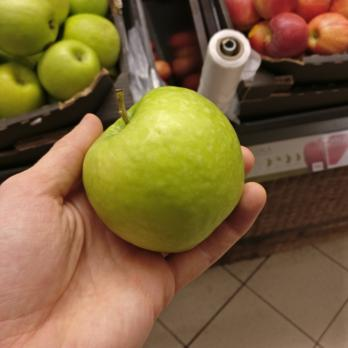
\includegraphics[width=30pt]{Chapter1/pics_paperA/Granny-Smith_021.jpg}}};
				\end{scope}
				\begin{scope}[xshift=34pt]
					\node {\fbox{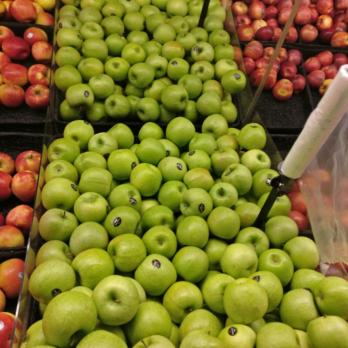
\includegraphics[width=30pt]{Chapter1/pics_paperA/Granny-Smith_012.jpg}}};
				\end{scope}
		\end{tikzpicture} }& 
		\makecell{\begin{tikzpicture}
				\begin{scope}
					\node {\fbox{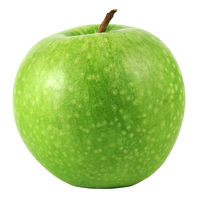
\includegraphics[width=30pt]{Chapter1/pics_paperA/Granny-Smith_Iconic.jpg}}};
				\end{scope}
		\end{tikzpicture} } & 
		\begin{scriptsize}
			\makecell{ \textit{“...\textbf{green} apple with \textbf{white, firm} pulp } \\[-1pt]  \textit{and a \textbf{clear acidity} in the flavor.”} } 
		\end{scriptsize}
		\\
		\hline 
		\makecell{ \scriptsize Tropicana \\[-1pt] \scriptsize Mandarin \\[-1pt] \scriptsize (Juice)}
		&  \makecell{ \begin{tikzpicture}
				\begin{scope}
					\node {\fbox{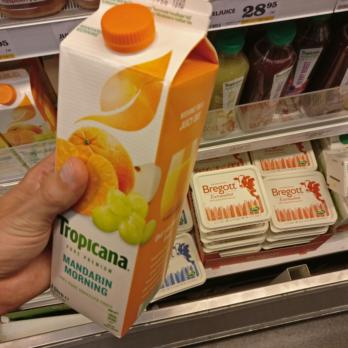
\includegraphics[width=30pt]{Chapter1/pics_paperA/Tropicana-Mandarin-Morning_003.jpg}}};
				\end{scope}
				\begin{scope}[xshift=34pt]
					\node {\fbox{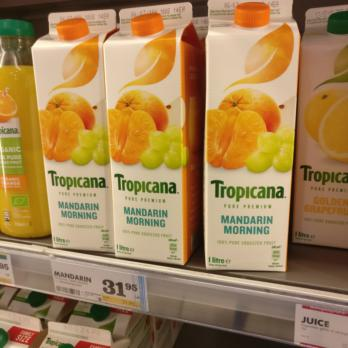
\includegraphics[width=30pt]{Chapter1/pics_paperA/Tropicana-Mandarin-Morning_016.jpg}}};
				\end{scope}
		\end{tikzpicture} }& 
		\makecell{\begin{tikzpicture}
				\begin{scope}
					\node {\fbox{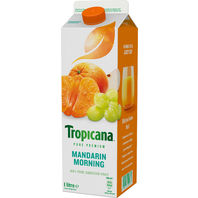
\includegraphics[width=30pt]{Chapter1/pics_paperA/Tropicana-Mandarin-Morning_Iconic.jpg}}};
				\end{scope}
		\end{tikzpicture} } & 
		\begin{scriptsize}
			\makecell{ \textit{“…is a \textbf{ready to drink} juice} \\[-1pt]
				\textit{\textbf{without pulp} pressed on \textbf{orange},} \\[-1pt]
				\textit{ \textbf{mandarin} and \textbf{grapes}. Not from} \\[-1pt]
				\textit{concentrate. Mildly \textbf{pasteurized}.” } }
		\end{scriptsize}
		\\
		\hline
	\end{tabular}
	%}
	\label{tab:paperA}
	\vspace{-3mm}
\end{table}




\begin{enumerate}
	\item[] \textbf{Marcus Klasson}, Cheng Zhang, Hedvig Kjellström. In \textit{IEEE Winter Conference on Applications of Computer Vision (WACV) 2019}.
\end{enumerate}

\paragraph{Summary}
We collect a dataset with natural images of raw and refrigerated grocery items taken in grocery stores in Stockholm, Sweden, for evaluating image classification models on a challenging real-world scenario. The data collection was performed by taking photos of groceries with a mobile phone to simulate a scenario of grocery shopping using an assistive vision app. Furthermore, we downloaded iconic images and text descriptions of each grocery item by web-scraping a grocery store website to enhance the dataset with information describing the semantics of each individual item. The items are grouped based on their type, e.g., apple, juice, etc., to provide the dataset with a hierarchical labeling structure. We show two examples of grocery item classes and their corresponding web-scraped information in Table \ref{tab:paperA}. 

We provide benchmark results evaluated using pre-trained and fine-tuned CNNs for image classification. Moreover, we take an initial step towards utilizing the rich product information in the dataset by training the classifiers with representations where both natural and iconic images have been combined through a multi-view VAE. 


\paragraph{Author Contributions}
CZ and HK presented the idea and the data collection procedure for the natural images and web-scraped information. MK performed the data collection including visiting the grocery stores for taking the natural images and the web-scraping of the grocery store website for iconic images and text descriptions. MK performed all the experiments. All authors contributed to discussing the results and contributed to writing the manuscript. 


\subsection{\underline{Paper B}: Using Variational Multi-View Learning for Classification of Grocery Items}
\label{sec:paperB}

\begin{comment}
	

\begin{figure}[t]
	\centering
	\begin{subfigure}[b]{0.3\textwidth}
		\centering
		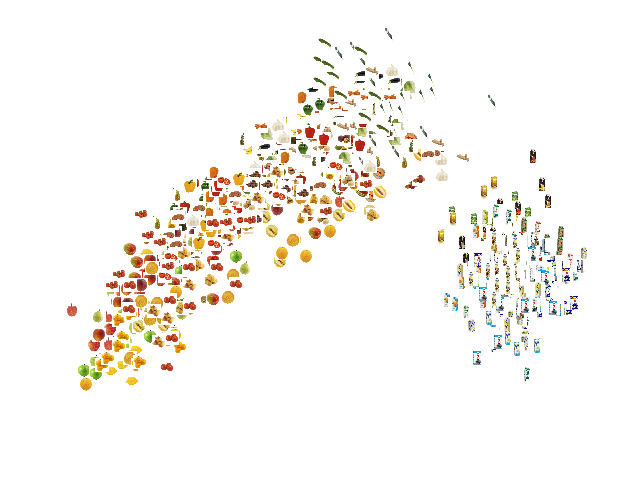
\includegraphics[width=\textwidth]{Chapter1/pics_paperB/pca_latents_vae_seed2}
		\vspace{-7mm}
		\caption{VAE$_{\vx}$}
		\label{fig:pca_latents_vae}
	\end{subfigure} 
	\hspace{-5mm}
	%\hfill
	\begin{subfigure}[b]{0.3\textwidth}
		\centering
		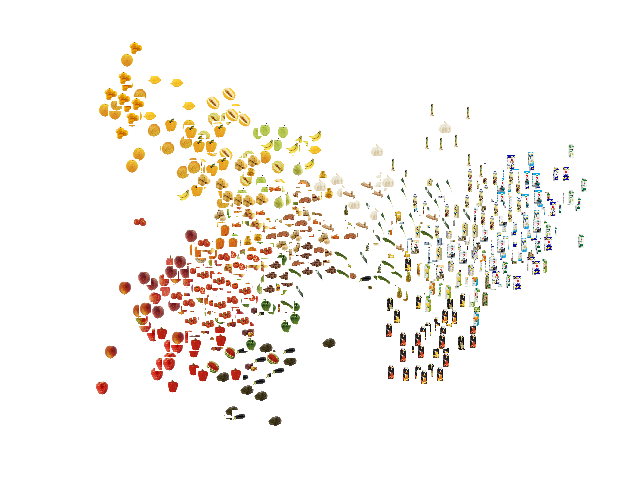
\includegraphics[width=\textwidth]{Chapter1/pics_paperB/pca_latents_vcca_xiwy_seed2}
		\vspace{-7mm}
		\caption{VCCA$_{\vx \vi \vw \vy}$ }
		\label{fig:pca_latents_vcca_xiwy}
	\end{subfigure}
	\vspace{-2mm}
	\captionsetup{width=.56\textwidth}
	\caption{Visualizations of the latent representations projected in 2D space with PCA from models VAE$_{\vx}$ and VCCA$_{\vx \vi \vw \vy}$. We plot the corresponding iconic image for each latent representation for visualization purposes. We observe that VCCA$_{\vx \vi \vw \vy}$ structures the items based on visual similarities by incorporating the web-scraped information into the latent representations, while VAE$_{\vx}$ only manages to separate the items into two clusters of raw and packaged items. }
	\label{fig:paperB_pca_latents}
\end{figure}
\end{comment}

%Visualizations of the latent representations from the test set, where we plot the iconic image of the corresponding object classes. We also plot the PCA projection of the natural image features from the off-the-shelf DenseNet169 in Figure \ref{fig:pca_densenet}. All models have been initialized with the same random seed before training. Abbreviations: VAE, Variational Autoencoder; VCCA, Variational Canonical Correlation Analysis.

%Visualizations of the latent representations $\mu_{z}$ of the red and green apples in the Grocery Store dataset. The red points correspond to the red apple classes, while the green points correspond to the green apple. The blue points correspond to the other grocery items. Abbreviations: VCCA, Variational Canonical Correlation Analysis.

\begin{enumerate}
	\item[] \textbf{Marcus Klasson}, Cheng Zhang, Hedvig Kjellström. In \textit{Patterns, Volume 1(8) (2020)}.
\end{enumerate}

\paragraph{Summary} 
We investigate whether training image classifiers can benefit from learning joint representations of grocery items using multi-view learning over the natural images and web-scraped information of the grocery items in the Grocery Store dataset (see Paper \ref{sec:paperA}). We employ a deep multi-view model based on VAEs called Variational Canonical Correlation Analysis (VCCA)~\cite{wang2016deep} for learning joint representations of the different data types, i.e., natural images, iconic images, and text descriptions. We performed a thorough ablation study over all data types to demonstrate how they contribute individually to enhancing the classification performance. Furthermore, we apply two classification approaches where we (i) train the classifier on the joint latent representations, and (ii) using a generative classifier by incorporating a class decoder to the VCCA model that can be used for classifying images. 

\begin{wrapfigure}[14]{r}[-4mm]{0.5\textwidth}
	\centering
	\vspace{-5mm}
	\begin{subfigure}[b]{0.26\textwidth}
		\centering
		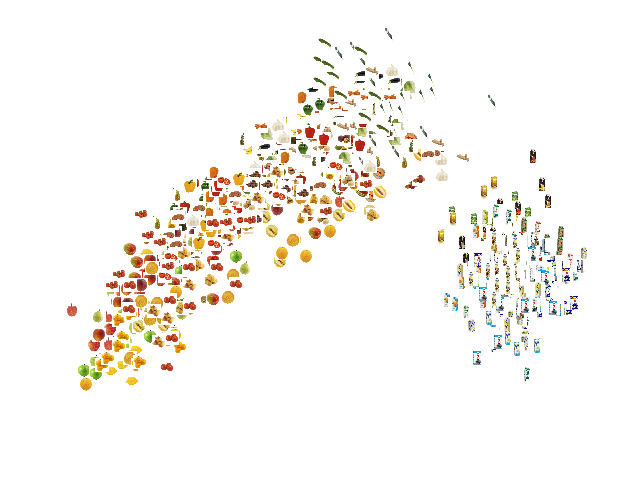
\includegraphics[width=\textwidth]{Chapter1/pics_paperB/pca_latents_vae_seed2}
		\vspace{-7mm}
		\caption{VAE$_{\vx}$}
		\label{fig:pca_latents_vae}
	\end{subfigure} 
	\hspace{-5mm}
	%\hfill
	\begin{subfigure}[b]{0.26\textwidth}
		\centering
		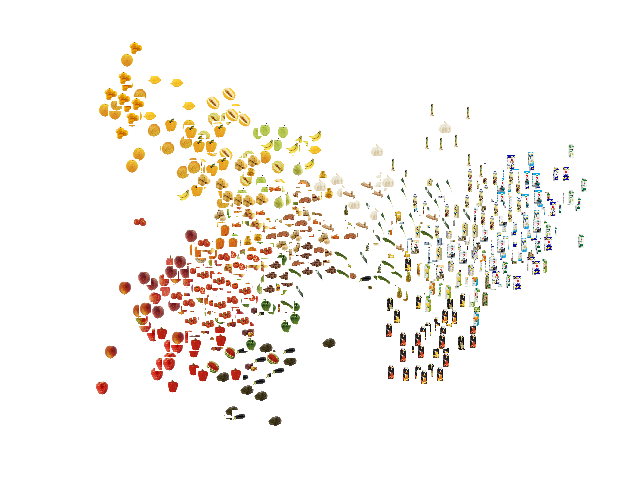
\includegraphics[width=\textwidth]{Chapter1/pics_paperB/pca_latents_vcca_xiwy_seed2}
		\vspace{-7mm}
		\caption{VCCA$_{\vx \vi \vw \vy}$ }
		\label{fig:pca_latents_vcca_xiwy}
	\end{subfigure}
	\vspace{-6mm}
	\captionsetup{width=.46\textwidth}
	\caption{Visualizations of the latent representations projected in 2D space with PCA from models VAE$_{\vx}$ and VCCA$_{\vx \vi \vw \vy}$, where we plot the corresponding iconic image for each latent representation. 
	%for visualization purposes. 
	We observe that VCCA$_{\vx \vi \vw \vy}$ structures the items based on visual similarities by incorporating the web-scraped information into the learning. 
	%We observe that VCCA$_{\vx \vi \vw \vy}$ structures the items based on visual similarities by incorporating the web-scraped information into the latent representations, while VAE$_{\vx}$ only manages to separate the items into two clusters of raw and packaged items. 
	}
	%\vspace{-3mm}
	\label{fig:paperB_pca_latents}
\end{wrapfigure} 
We performed a thorough ablation study over all data types to demonstrate how they contribute individually to enhancing the classification performance. To gain further insights into our results, we visualized the learned representations of the grocery items from VCCA and discussed how the iconic images and text descriptions help the model to better distinguish between the groceries. Our results show that the iconic images help to group the items based on their color and shape while text descriptions separate the items based on differences in ingredients and flavor. Figure \ref{fig:paperB_pca_latents} shows visualizations of the latent representations projected in 2-dimensional space using Principal Component Analysis (PCA), where we illustrate how the latents change when adding the iconic image and text description into the VCCA model. Finally, we concluded that utilizing the iconic images and text descriptions yielded better classification results than only using natural images. 


\paragraph{Author Contributions} 
CZ and HK presented the idea and all authors contributed to formalizing the methodology. 
MK performed all the experiments and created the visualizations. 
All authors took part in discussing the results.
All authors contributed to writing the manuscript. 


\subsection{\underline{Paper C}: Learn the Time to Learn: Replay Scheduling for Continual Learning}
\label{sec:paperC}

\begin{figure}[h]
	\centering 
	\includegraphics[width=0.33\textwidth]{example-image-c}
	\caption{ \MK{Paper C could illustrate the new CL setup with a figure that shows a network and a scheduler that needs to fetch a small replay memory from a huge pool of historical data.}}
	\label{fig:paperC}
\end{figure}

\begin{enumerate}
	\item[] \textbf{Marcus Klasson}, Hedvig Kjellström, Cheng Zhang. Submitted to \textit{International Conference on Machine Learning (ICML) 2022}.
\end{enumerate}

\paragraph{Summary}
In this paper, we show that learning the time to replay different tasks can be critical for continual learning (CL) performance in replay-based methods. As the main assumption in replay-based CL is that only a small set of historical data can be re-visited for mitigating catastrophic forgetting, most works have focused on improving the sample quality of the replay memory. However, in many real-world applications, historical data is accessible at all times, e.g., by storing it on the cloud. But although all historical data could be stored, retraining machine learning systems on a daily basis is prohibitive due to processing times and operational costs. Therefore, small replay memories are still needed in CL to mitigate catastrophic forgetting when learning new tasks. To this end, we propose to learn the time to learn for a CL system, in which we learn schedules over which tasks to replay at different times. Inspired by human learning, we demonstrate that scheduling over the time to replay is critical to the final CL performance with finite memory resources. We then illustrate our idea with scheduling over which tasks to replay by learning such policy with Monte Carlo tree search. We perform extensive evaluation showing that learning replay schedules can significantly improve the performance compared to baselines without learned scheduling. We also show that our method can be combined with any replay-based method and memory selection technique. Finally, our results indicate that the learned schedules are also consistent with human learning insights.



\paragraph{Author Contributions} 
CZ presented the idea and MK and CZ contributed to formalizing the methodology. 
MK performed all the experiments. 
All authors took part in discussing the results and contributed to writing the manuscript. 


\subsection{\underline{Paper D}: Meta Policy Learning for Replay Scheduling in Continual Learning}
\label{sec:paperD}

\begin{figure}[h]
	\centering 
	\includegraphics[width=0.33\textwidth]{example-image-golden}
	\caption{ \MK{Paper D could show illustration of the RL agent scheduler that gets performance measures as input and outputs an action proportion of how to select the replay memory. RL agent could also have a replay buffer where data is collected from several environments. Maybe it can also show the test case, so that it would be two separated "at training/test phase". }}
	\label{fig:paperD}
\end{figure}

\begin{enumerate}
	\item[] \textbf{Marcus Klasson}, Hedvig Kjellström, Cheng Zhang. Under preparation for conference submission.
\end{enumerate}



\paragraph{Summary} 
In this paper, we propose a reinforcement learning-based method for learning policies for replay scheduling that can be applied in new continual learning scenarios. We demonstrated in Paper C that learning the time to replay different tasks is important in continual learning. However, a replay scheduling policy that can be applied in any continual learning scenario is currently absent, which makes replay scheduling infeasible in real-world scenarios. To this end, we propose using reinforcement learning to enable learning general policies that can generalize across different data domains. 
The learned policy can then propose replay schedule that efficiently mitigate catastrophic forgetting to improve the continual learning performance without any additional computational cost in the new domain. We compare the learned policies to several replay scheduling baselines and show that the learned policies can improve the continual learning performance given task orders and datasets unseen during training. 


\paragraph{Author Contributions} 
CZ presented the idea and MK and CZ contributed to formalizing the methodology. 
MK performed all the experiments. 
All authors took part in discussing the results and contributed to writing the manuscript. 



% Thesis outline
\section{Thesis Outline}\label{sec:outline}
The rest of the thesis is organized as follows. We provide some background and preliminaries on the machine learning methodology used in this thesis in Chapter \ref{chap:background}. Chapter \ref{chap:finegrained_classification} is focused on our contributions in fine-grained classification where we first describe the related work in this field followed by explaining the frameworks used in our work. Similarly, in Chapter 4, we focus on our contributions in continual learning by first describing the related work to place our contributions in context and then describing the framework we used for enabling replay scheduling in continual learning. Finally, in Chapter 5, we provide our conclusions of the presented works and present some research directions that we believe would be interesting to look deeper into in the future. 

\MK{todo: fix references to chapters!}
%*******************************************************************************
%*********************************** Second Chapter ****************************
%*******************************************************************************

\chapter{Background}
\label{chap:background}

The goal with this chapter is to provide the reader with preliminaries that are useful for comprehending the included papers. We assume that the reader has some knowledge in calculus, linear algebra, and probability theory, but we intend to keep it on a basic level. First, we give the notation that will be used throughout the thesis. Then, we will introduce a selection of related works to place the thesis into context. 

\section{Notation and Terminology}\label{sec:notation}

We will begin by providing some algebraic notation that will be used for representing various types of data in the thesis. Scalars (both integer and real) are denoted by italic letters such as $a$. Vectors are denoted by lowercase bold italic letters such as $\vx$, where all vectors are assumed to be column vectors. A superscript $T$ denotes the transpose of a vector or matrix, such that $\vx^{T}$ becomes a row vector. Matrices are denoted as uppercase bold italic letters such as $\mW$. The notation $(w_1, \dots, w_m)$ denotes a row vector with $m$ elements, where the corresponding column vector is denoted as $(w_1, \dots, w_m)^{T}$. 

A dataset is denoted by the set $\gD = \{\vx^{(1)}, \dots, \vx^{(N)} \}$, where $\vx^{(i)}$ is the $i$-th example among the $N$ data points. Each data point is assumed to belong in a space of vectors denoted by $\gX$, such that $\vx \in \gX$. The data generating distribution is denoted by $p_{data}(\gX)$ which is usually unknown. To provide an example, we let the vector $\vx = (x_1, \dots, x_m)$ represent a flattened image of $m$ pixels. In this case, all possible images that can exist belong to the space $\gX$ and the data generating distribution $p_{data}(\gX)$ gives the probability of how likely each image is to occur in the world. In supervised learning, there is also a target, either denoted as $y^{(i)}$ or $\vy^{(i)}$, associated with $\vx^{(i)}$. The target belongs to the target space $\gY$, where the space is discrete $\gY = \{1, \dots, C\}$ for classification tasks over $C$ number of classes, or continuous $\gY = (-\infty, \infty)$ over an interval of real values for regression tasks. 

%Perhaps can skip spaces and use $\vy \in \{1, \dots, C\}$ to represent the labels and $\vx \in \mathbb{R}$, since I don't really use $\gX$ anywhere but in the RL part for state and action spaces but perhaps it's good to introduce the space notation then...

Throughout this thesis, we take a machine learning approach to solve tasks by tuning an adaptive model using a dataset called the \textit{training set}. In our case, we will represent the model with a function $f_{\vtheta}(\vx)$ that allows us to predict outcomes of events/data $\vx$ from the task of interest. The parameters $\vtheta$ expresses the function and we use machine learning algorithms for tuning parameters with the given dataset during the training phase. Once the model is trained, we often enter the \textit{test phase} where we want to evaluate the model by predicting outcomes on an unseen dataset called the \textit{test set}. The ability to predict outcomes of new data that is different from the examples seen during training is called \textit{generalization}, which is a central goal for most applications in machine learning and pattern recognition. 


\section{Problem Settings in Machine Learning}

Machine learning problems can be divided into three main fields, namely, \textit{supervised learning}, \textit{unsupervised learning}, and \textit{reinforcement learning} (RL). Since this thesis includes work from each of these problem settings, we will briefly introduce these topics to provide the reader with context on the tasks that we are trying to solve. 

\MK{TO-DO: Add references to papers and sections!}
\paragraph{Supervised Learning.} In this setting, we are given a dataset $\{(\vx^{(i)}, \vy^{(i)})\}_{i=1}^{N}$ where each data example $\vx^{(i)}$ is accompanied with a target $\vy^{(i)}$. The goal is to estimate a function $f_{\vtheta}(\vx)$ that assigns the correct target to each example in the training set as accurately as possible. In classification problems, each target belongs to one of $K$ discrete categories, such that $\vy = \{1, \dots, K\}$, and we want to predict which of the categories that new data belongs to. Classification tasks will be involved in all included papers of this thesis wherein Paper \ref{chap:paperA} and B we focus on assigning the correct product category to images of grocery items. Another problem type in supervised learning is regression where the targets are continuous and real-valued. An example of a regression task is to predict the outdoors temperature tomorrow given the observed temperature today. 

\paragraph{Unsupervised Learning.} Here, we are given a dataset $\{\vx^{(i)}\}_{i=1}^{N}$ without access to any corresponding targets. The goal in this unsupervised setting may then be to find hidden structures in the given dataset. For example, we might be interested in discovering groups of similar examples with \textit{clustering} techniques, or we may want to use \textit{density estimation} where we approximate the true data distribution $p_{data}$ with a parametric distribution $p_{\vtheta}$ using the collected dataset, or we may want to project high-dimensional data into two or three dimensions for \textit{visualization} purposes. We will get back to these goals when we introduce representation learning in Section X. 

\paragraph{Reinforcement Learning.} For these problems, we have a \textit{learning agent} that wants reach a goal in an environment by performing a given set of actions. After performing an action, the agent observes the state of the environment and receives a reward from the environment saying how good or bad the taken action was to reach the goal. The objective for the agent is to maximize the reward signal within the time the agent reaches the goal. The agent then has to learn a policy for deciding which actions to perform in certain situations in the environment. The policy $\pi_{\vtheta}(\va | \vs)$ is a mapping from perceived states $\vs$ in the environment to actions $\va$ that should maximize the reward signal. An example of a task that can be framed as a RL problem is the so called Mountain Car problem, where the agent is a car that is trying to drive up to the top of a hill. The state represents the position and velocity of the car and the agent must take actions that will move the car forward or backwards. The objective is to reach the goal with as little time as possible, and the agent is encouraged to do so by the environment by sending the agent a negative reward for every time step that passes without reaching the top of the hill. We will return to the RL framework later when we describe the prerequisites for Paper D. \vspace{1mm}

There exist many different methods for solving problems within these three fields. In this thesis, we employ deep learning methods which has been successfully applied in each field by representing the models with deep neural networks~\cite{he2016deep, bengio2013representation, mnih2015human}.

%that is trying to maximize a reward signal $r$ by performing a given set of actions in an environment to reach a specific goal. The agent observes the state of the environment 


%In this paradigm, we are concerned with decision-making where the goal is to take actions that maximize some reward. The decision-making is modeled by a policy which bases the action selection on observations that are collected by interacting with the task environment through the selected actions. One main challenge is how to handle the trade-off between exploration of different actions in new situations and exploitation by selecting actions where the agent already has experienced good reward signals. Furthermore, the reward signal can be received either in dense or sparse forms, where sparse rewards are typically more challenging to learn from and are less sample-efficient. 


\section{Deep Learning}

In this section, we give a brief overview of deep learning~\cite{goodfellow2016deep} which is the main building block for the models we use in this thesis. Deep learning contains a family of machine learning models based on neural networks that are parametric function approximators used for representing some function of interest. Much of the successes of deep learning methods have been in supervised learning settings, especially in applications where there are large amounts of labelled data and sufficiently large model in terms of number of parameters in the network. In the following sections, we will introduce the deep learning frameworks and models that we have used in this thesis.   

%For many applications, neural networks have been shown to  that are used for representing functions  are parametric function approximators. 

\subsection{Deep Neural Networks}

Neural networks is a class of machine learning models which popularity have grown immensely due to their ability to learn from large and high-dimensional datasets. Moreover, neural networks have been successfully applied in various number of fields in computer vision~\cite{he2016deep, krizhevsky2012imagenet}, natural language processing~\cite{devlin2018bert}, and reinforcement learning~\cite{mnih2015human, silver2016mastering}. These models are constructed by stacking layers of parameters that extract intermediate representations of the input data. The last layer outputs the target answer from the queried input and is specific for the task. For example, in image classification, the last layer outputs class scores representing which class the image is most likely to belong to. 

Next, we will describe three popular types of neural networks, namely, multilayer perceptrons (MLPs), convolutional neural networks (CNNs), and recurrent neural networks (RNNs). \MK{TO-DO: It would be nice to have some simple illustrations of how the networks process the data, I can take inspiration from how other people have done it.}

\paragraph{Multilayer Perceptrons.} The simplest form of feedforward neural networks is the MLP. Let the vector $\vx = (x_1, \dots, x_d)^{T}$ be some form of data where $x_i$ is the $i$-th feature for $i = 1, \dots, d$. Every layer in the MLP constitutes of weights $\mW$ that are used for transforming the input such that the output reveals some hidden structure useful for solving the task of interest. The transformation is performed with a matrix multiplication, i.e., $\vh = \mW \vx$, to receive the intermediate representation $\vh$. An essential part for enabling neural networks to learn non-linear functions is to add an activation function right after the matrix multiplication of each layer. Otherwise, the neural network would only be capable of learning linear functions since the matrix multiplication is a linear mapping. A common activation function is the $a(\vx) = \max(0, \vx)$, or the so called Rectified Linear Unit (ReLU) activation, which outputs $\vx$ when $\vx > 0$ or otherwise zero. By stacking two layers together in a neural network with a ReLU activation, we then obtain the representation $\vh = \mW_2\max(0,  \mW_1\vx)$. Note here that this representation could be predicted class scores, such that $\vh = \hat{\vy}$, if we would use two-layer MLP for a classication task. 

\paragraph{Convolutional Neural Networks.} For data where the spatial order of each feature can be salient for prediction tasks such as image classification, we need a network that can capture relationships between features. CNNs are special kinds of neural networks that can process data with grid-like structures. Convolutional layers constitutes of a set of filters with adaptable weight parameters. To produce the output, we slide each filter across the input across the width and height of the input and compute dot products between the filter weights and the input at any position. Each filter will then produce a 2-dimensional feature map that gives the responses of that filter at every spatial position. The 2-dimensional feature maps from all filters are then stacked depth-wise to obtain the output volume. The obtained feature maps are often downsampled along their spatial dimensions using a pooling operation after the activation function. The parameter sharing in convolutional layers where each weight in a filter is applied to every position of the input comes from the idea that if some visual features are important in one part of the image, it should intuitively be useful at some other location as well. Furthermore, this design choice also makes the model require fewer parameters and a lower number of operations to compute the outputs.

%Intuitively, the network will learn filters that activate when they see some type of visual feature such as edges in early layers, and eventually object parts in later layers that are discriminative . 

%Convolutional layers provide three important properties that can help the model, namely, sparse interactions, parameter sharing, and equivariant representations~\cite{goodfellow2016deep}. In MLPs, the matrix multiplication makes every output unit interact with every input unit. In contrast, CNNs typically establishes sparse interactions between the output and input by making the filter smaller than the input. This means that the model needs fewer parameters and fewer number of operations to compute the output. Furthermore, each weight is applied to every position of the input (except perhaps boundary pixels depending design choices of the layer) compared to in MLPs where a weight is multiplied with one element and never revisited.   

%An intuitive example is to detect edges in an image with pixels around local region rather than using pixels 

%Each filter operates on local regions of the input by computing the dot product between the weights and the local input region. The output is a feature map obtained by computing the dot product between the weights and the input by sliding the filter weights across the whole input.  same weights are slid across the whole input to obtain a feature map weights in a filter , where the dot product of the  

%, we The MLP operates on each input feature individually. Hence, the order of the features is ignored. However, in images, we know that pixels can have strong relationships between each other where, for instance, two neighboring pixels often have similar color and may belong to the same object that we wish to recognize. 


\paragraph{Recurrent Neural Networks.} RNNs are a family of neural network models specialized for processing sequences of data. Similar to CNNs, these models use parameter sharing by applying the same weights across several time steps. The parameter sharing is important in RNNs as it enables the model to handle different sequence lengths as well as being capable of recognizing relevant information that can appear at different locations in the sequence. Many RNNs follow the same procedure through the equation $\vh^{(t)} = f_{\vtheta}(\vh^{(t-1)}, \vx^{(t)})$, where the RNN produces the current state $\vh^{(t)}$ by incorporating the input data $\vx^{(t)}$ at time $t$ into the previous hidden state $\vh^{(t-1)}$. Hence, the hidden state $\vh^{(t)}$ will now contain information about the whole past sequence up to time $t$. In most applications, there will be an extra output layer that reads the information from state $\vh^{(t)}$ to make predictions. An example application for RNNs is predicting the next word in a sentence given previous words, where the RNN should store the necessary information about previous words to predict the rest of the sentence. A common choice of RNN model is the Long Short-Term Memory~\cite{hochreiter1997long} (LSTM) which mitigates problems with vanishing gradients during the training phase. \vspace{1mm}

For training deep networks, \textit{loss} functions are used for measuring how well the network performs to solve the task of interest. In classification tasks, the cross-entropy loss is commonly used where the predicted class scores $\hat{\vy}$ are compared against the true target class $\vy$,
\begin{align}
	\gL_{CE}(\hat{\vy}, \vy) = -\sum_{k=1}^{K} \vy[k] \log \hat{\vy}[k],
\end{align}
where the true target vector $\vy$ uses a one-hot representation where the true class $i$ is denoted in the vector by setting the $i$-th element in $\vy$ to one, as in $\vy[i] = 1$, and zero elsewhere. 

Probably the most common optimization algorithm for deep learning is stochastic gradient descent (SGD). The model parameters are updated by first computing the gradient of the loss function with respect to the weights of the network, as in $\nabla_{\vtheta} \gL(f_{\vtheta}(\vx), \vy)$, for a single input-output pair with backpropagation~\cite{rumelhart1986learning}. We can then update the parameters with the equation 
\begin{align}\label{eq:weight_update_sgd}
	\vtheta = \vtheta - \eta \nabla_{\vtheta} \gL(f_{\vtheta}(\vx), \vy),
\end{align} 
where $\eta$ is the learning rate which is an important parameter for SGD determining how much the weights should be updated with the computed gradient. 



\subsection{Deep Autoencoders}

A common architecture type for deep learning in unsupervised learning are autoencoders for learning hidden representations of unlabeled data. Autoencoders are commonly used for dimensionality reduction of high-dimensional data, where the lower-dimensional representation can be used for classification tasks, or to visualize hidden structures in the data that are hard to reveal from the original input data. The objective of the model is to reconstruct the original input data. The network architecture is built using two networks called \textit{encoder} and \textit{decoder} with a bottleneck layer between the networks for extracting the hidden representation $\vh$. The encoder and decoder architectures can be of any neural network type, such as MLPs, CNNs, or RNNs, that fits the given dataset. The encoder is used for obtaining the hidden representation of the input data, while the decoder tries to reconstruct the original input from the obtained representation. Therefore, the idea is that the learned representation should contain the relevant information for reconstructing the data. 

Mathematically, we denote the decoder as $f_{\vtheta}$ and the encoder as $g_{\vphi}$. The encoder extracts the hidden representation $\vh = g_{\vphi}(\vx)$ from the input $\vx$, then the decoder produces a reconstruction $\hat{\vx} = f_{\vtheta}(\vh)$ from $\vh$. We train the encoder and decoder simultaneously by minimizing a reconstruction loss $\gL(f_{\vtheta}(g_{\vphi}(\vx)), \vx)$, for instance mean-squared error loss, using SGD similarly as for the feedforward networks described above. There exist various kinds of methods for improving the quality of the learned representations in autoencoders. For example, we can adjust target task by adding noise to the inputs and let the decoder reconstruct the original input from noise variants~\cite{vincent2008extracting}, or we can induce different constraints in the bottleneck layer to, for example, obtain a sparse lower-dimensional representation of the data. Next, we will introduce the variational autoencoder which originates from latent variable models. 

\subsubsection{Variational Autoencoders}

The variational autoencoder~\cite{kingma2013auto} (VAE) is a variant of autoencoders where learning is viewed from the perspective of probabilistic modeling. These models come from the family of deep generative models, where the goal is to approximate some underlying data distribution $p_{data}$ with a parametric distribution $p_{\vtheta}$ learned from a dataset $\gD \sim p_{data}$. A common approach for estimating $p_{\vtheta}$ is to use a latent variable model that infers hidden structures in the data to facilitate learning the distribution. VAEs is a deep latent variable model that uses neural networks for learning $p_{\vtheta}$ making the training scalable to large high-dimensional datasets. 

The main idea with introducing latent variables is that they should encode some semantically meaningful information about the observed data. Latent variable models are usually expressed by the joint distribution 
\begin{align}
	p_{\vtheta}(\vx, \vz) = p_{\vtheta}(\vx | \vz) p(\vz),
\end{align}
where $\vz$ denotes the latent variables and $\vx$ the observed variables that represents the observed data points. The distribution $p_{\vtheta}(\vx | \vz)$ is the likelihood of the data and $p(\vz)$ is the prior distribution for the latents. This model describes the generative process of the data $\vx$ by following the steps 1) sample the latent vector $\vz \sim p(\vz)$ from the prior, and 2) generate data point $\vx \sim p(\vx | \vz)$ from the sampled latent $\vz$. We are now interested in learning the model $p_{\vtheta}(\vx, \vz)$ that best fits a given dataset $\gD$, as well as inferring the posterior distribution $p_{\vtheta}(\vz | \vx)$ over the latent variables $\vz$ given the data $\vx$.

The overall goal with latent variable models is to maximize the marginal log-likelihood $\log p_{\vtheta}(\vx)$ given a dataset $\gD \sim p_{data}$. However, computing $p_{\vtheta}(\vx)$ by with marginalizing out the $\vz$ from the model $p_{\vtheta}(\vx) = \int p_{\vtheta}(\vx, \vz) \, d\vz$ is in general intractable due to the many settings of $\vz$ we would need to evaluate. Consequently, the posterior distribution also becomes intractable since $p_{\vtheta}(\vz | \vx) = p_{\vtheta}(\vx, \vz) / p_{\vtheta}(\vx)$ from Bayes' rule. Variational inference~\cite{zhang2018advances, blei2017variational} is a technique for enabling learning of latent variable models. The idea of variational inference is to provide means for calculating the marginal log-likelihood $\log p_{\vtheta}(\vx)$ by selecting a parameterized distribution $q_{\vphi}$ for approximating the true posterior distribution. In VAEs, the approximate posterior $q_{\vphi}(\vz | \vx)$ is represented as a neural network with parameters $\vphi$ that outputs the latents $\vz$ given data points $\vx$. With this approach, we can now form a lower bound on the marginal log-likelihood given by 
\begin{align}
	\log p_{\vtheta}(\vx) \geq \E_{z \sim q_{\vphi}(\vz | \vx)}[\log p_{\vtheta}(\vx | \vz)] - \KL[q_{\vphi}(\vz |  \vx) \, || \, p(\vz)] . 
\end{align}
The right-hand side is called the evidence lower bound (ELBO) and comprises of two quantities that we can evaluate to train the model. The expectation over the log-likelihood $\log p_{\vtheta}(\vx | \vz)$ can be estimated with Monte Carlo sampling. The KL divergence between $q_{\vphi}(\vz |  \vx)$ and $p(\vz)$ can be computed analytically depending on how we choose these distributions. The standard choice for the prior is to use a zero-mean unit-variance Gaussian distribution $p(\vz) = \gN(\vz; \bm{0}, \mathbf{I})$ where $\mathbf{I}$ is the identity matrix. The approximate posterior is also selected to be a Gaussian distribution $q_{\vphi}(\vz | \vx) = \gN(\vz; \vmu_{\vphi}(\vx), \text{diag}(\vsigma_{\vphi}(\vx)))$, where the encoder network parameterized by $\vphi$ outputs the the means $\vmu_{\vphi}(\vx)$ and standard deviations $\vsigma_{\vphi}(\vx)$ for the latent dimensions. The latent vector is sampled using the "reparametrization trick"~\cite{rezende2014stochastic, kingma2013auto} by computing $\vz = \vmu_{\vphi}(\vx) + \vepsilon \odot \vsigma_{\vphi}(\vx)$, where $\vepsilon \sim \gN(\bm{0}, \mathbf{I})$ and $\odot$ denotes element-wise multiplication, which enables backpropagating gradients through the sampling operation. The likelihood $p_{\vtheta}(\vx | \vz)$ is the decoder network that tries to reconstruct the original input to the encoder. The likelihood distribution depends on the type of data $\vx$ we wish to generate. If $\vx$ is a continuous variable, then we can let the decoder output Gaussian parameters for the likelihood similar as for the encoder. 

VAEs have been used in various applications for modeling images, text, and audio data, as well as when combining data from different modalities. Next, we will briefly introduce how autoencoders can be used when learning representations from multiple data types from different modalities. 



\subsubsection{Multimodal Learning using Autoencoders}

Learning representations from different types of data is a highly active research field in deep learning~\cite{baltruvsaitis2018multimodal}. Combining visual data with other modalities such as natural language and audio signals for learning more rich representations of data has been studied frequently the last decade~\cite{owens2018audio, ngiam2011multimodal, silberer2014learning, lee2020making} [Add REFs]. A common framework in such applications is to use autoencoders for incorporating information from the different data types into a single joint representation. Learning from multiple sources then opens up for capturing correspondences between the data types and obtaining better representations that can be used for downstream tasks such as classification. 

Let $\vx$ and $\vy$ originate from two different data sources but share some high-level information. For example, $\vx$ could be an image of a living room and $\vy$ is text describing the appearance of the room, where objects are located etc. Constructing a joint representation is then done by projecting both $\vx$ and $\vy$ with separate encoder networks into the same latent space. The joint multimodal representation is then passed through two separate decoder networks used for predicting the original input data individually. The advantage of multimodal autoencoders is that they can be trained end-to-end for both learning representations as well as making predictions of the used modalities. However, a major challenge is how to handle scenarios where modalities might be missing. One option is to only encode the data modality that we know will be available at both training and test phases and then establish a joint representation by decoding two both modalities~\cite{ngiam2011multimodal}.

Multimodal autoencoders have frequently been extended to deep generative models, mainly VAEs~\cite{wang2016deep, wu2018multimodal, shi2019variational, vedantam2017generative, suzuki2016joint}. These models are capable of generating new data through sampling from the latent space in addition to learning joint representations. Furthermore, they can handle missing modalities for the encoders which enables cross-modal data generation between the modalities. In Paper B [Add REF], we employ Variational Canonical Correlation Analysis (VCCA) for learning joint representations of natural images and web-scraped information of grocery items to facilitate learning image classifiers. 


\subsection{Deep Reinforcement Learning}
\MK{TO-DO: Related works for Paper D. After writing Chapter 4 on CL}

In this section, we give a brief overview to Reinforcement Learning~\cite{sutton2018reinforcement} (RL) and introduce some approaches for how to incorporate deep neural networks in RL. 

%% talk about notation, then go into DQN, actor-critic methods and PPO briefly

%  our goal will be to tune an adaptive model  


%The tasks of interest involves estimating some probability distribution from data. In classification tasks, we are given pairs $(\vx, \vy)$ of data with an associated target label and are asked to assign one of $k$ categories to input $\vx$. Hence, our goal is to estimate the conditional probability distribution $p(\vy | \vx)$ over the target label $\vy$ given the input data $\vx$. Commonly, the distribution $p_{\vtheta}(\vy | \vx)$ is parameterized by $\vtheta$. One can also write $p_{\vtheta}(\vy | \vx)$ as a function $f_{\vtheta}(\vx): \sR \rightarrow \{1, \dots, k\}$, such that $f_{\vtheta}(\vx) = p_{\vtheta}(\vy | \vx)$, where $f$ is a function that predicts target labels $\vy$ from inputs $\vx$ by performing a mapping between the input and target spaces. Our goal is to update the parameters $\vtheta$ such that they a loss function $\gL(\vtheta)$ is minimized. A typical loss for classification tasks is the cross-entropy loss which can be minimized by taking the gradient of $\gL$ w.r.t. the parameters $\vtheta$. 


%\MK{TO-DO: How to describe computing the loss and updating the parameters? Maybe the stanford CNN course has some nice explanations?}




%The goal with this thesis is to provide machine learning methods for recognizing objects from images. Machine learning is a field within Artificial Intelligence where computer programs learns from experiences how to make predictions in new situations. There are three essential parts to enable the computer to make predictions with machine learning. Firstly, we need data representing the scenarios where we have objects that we wish to predict what they are. Secondly, we need a model that learns how to make the decisions based on the provided data. Thirdly, we need a learning algorithm for fitting the model to the data we have such that good and sensible decisions can be made on future data. Machine learning has proven to be successful on various types of data, including, images and video, text, and audio, and there exists many different kinds of models and algorithms for learning decision-making from data. 

%One of the main goals with machine learning is to have models that generalize to unseen data and events. However, there are several challenges that has to be tackled to achieve this goal. The first challenge is to obtain datasets that represent the events that the model should make predictions for. Machine learning models often require vast amounts of examples to learn from, and also, the examples should be annotated with some information describing each example in order to ease the learning. But even if we have large datasets, we must have models that have the capacity of preserving the knowledge gained from the dataset. Furthermore, we must have algorithms that can train the model from the huge amount of data in computationally efficient both time- and processing-wise. Especially for visual data, it has become much cheaper to obtain vast amounts of images and videos from the internet. Occasionally, these can be annotated through search words or, alternatively, from crowdsourcing. Moreover, computational power has also become cheaper through smaller and more efficient micro-processors, semi-conductors, and cloud computing. Deep learning~\cite{goodfellow2016deep} is a class of machine learning models based on neural networks that are capable of learning from large and high-dimensional datasets due to their capacity. They are trained using an optimization algorithm called Stochastic Gradient Descent (SGD)~\cite{bottou2010large} which works well for large-scale data and can be applied on graphical processing units (GPUs) with recent machine learning programming libraries, such as TensorFlow, PyTorch, and Jax. However, deep learning still faces lots of challenges in generalization, especially when they are applied in environments that were not present in the training data, and it is still an open research problem on how to make them generalize better. 

%There are several approaches for enabling better generalization for deep learning models. A good start is to collect datasets that are similar and represent the events in the environment where the model will be deployed. Related to this, one can also collect different data types from various modalities, such as visual signals in the form of images and video as well as natural language which can be written or spoken, if these are available in the data collection process and are sensible for the task to be solved. Multimodal machine learning opens up the possibility of learning correspondences between the different data types to gain better understanding of the phenomenon of interest~\cite{baltruvsaitis2018multimodal, xu2013survey}, which can help the model to be more accurate and robust. However, in order to enhance the utility of machine learning models, they should be capable of continuously updating their knowledge as many environments where object recognition is useful are ever-changing~\cite{delange2021continual, parisi2019continual}. We should build models that can add new objects of interest to recognize as well as delete concepts that are obsolete or non-relevant. It would also be useful if we could update models with personalized objects to recognize to narrow down the scope of items to recognize for object recognizers to make the tasks easier.  

%In this chapter, we cover related works on datasets on object recognition both with image and text data in Section \ref{sec:datasets_for_object_recognition}. Next, we provide a description of machine learning, especially deep learning, models that were used in the included papers in Section \ref{sec:machine_learning} and \ref{sec:deep_learning}. In Section \ref{sec:continual_learning}, we discuss the setting of continual learning for updating the knowledge of machine learning models that is aiming to make the models capable of handling ever-changing environments as a step towards to enabling life-long learning. 

%\section{Machine Learning Basics}

%\section{Deep Learning}

%\subsection{Autoencoders}

%\section{Reinforcement Learning}

%\subsection{Monte Carlo Tree Search}

%Data -> Modeling -> Evaluation/Generalization

% Datasets for object recognition
%\section{Datasets for Object Recognition} % Visual Recognition?
\label{sec:datasets_for_object_recognition}

The increasing accessibility of large-scale image datasets have enhanced the possibility for applying machine learning in various applications for visual recognition. One of the most well-known datasets in computer vision the is Imagenet database~\cite{deng2009imagenet} introduced in 2009 which is still used for benchmarking models on large-scale image classification. Imagenet was collected through image search results from the Internet and then further assessed by crowdsourcers from Amazon Mechanical Turk to achieve higher quality of the collected images as well as labeling them. There has been several efforts to create more large-scale vision datasets, e.g., Pascal VOC~\cite{everingham2015pascal}, Microsoft COCO~\cite{lin2014microsoft}, Visual genome~\cite{krishna2017visual}, which in addition to object classes include object attributes, bounding boxes for detecting objects, and pixel-wise segmentation masks. Additionally, there exists datasets where images have been combined with text descriptions of things that are present and where they are located in relation to each other for image captioning and visual question answering tasks, e.g., Flickr30k~\cite{young2014image}, VQA~\cite{antol2015vqa}, GQA~\cite{hudson2019gqa}, and Microsoft COCO Captions~\cite{chen2015microsoft}. These publicly accessible datasets are one of the major reasons for enabling machine learning and computer vision research at a large scale which opens up for developing products that can be deployed on everyday products, such as mobile phones. 


In order to deploy machine learning models in real-world scenarios, we first need training data that are close to the occurring events specific for the application where the model will be used. 
But even if we can train a model on huge amounts of images, it is extremely challenging to provide examples that cover all possible scenario that can happen or every different shape and color an object can have. Furthermore, other circumstances such as lighting conditions, occlusions, and other objects in the surroundings of objects of interest which can be hard to control can also make the recognition performance less accurate. This is critical when training models where the user is strongly relying on the recognition performance, such as in assistive vision systems for blind or low-vision people. As many of the popular image datasets for computer vision contains images from the Internet, there can be a large gap between the training images and the images that will be seen after deployment as Internet images often have good conditions and the objects are fully visible and centered. However, when the model would be used in the real-world, the objects could be occluded or not fully visible in the image and be disturbed by objects in the background. Therefore, it can be critical for the performance and robustness of the model to train it on images that are tailored for the scenarios where it will be applied. 

There have been several attempts to build datasets with images collected by visually impaired to obtain more realistic datasets with potential scenarios. VizWiz~\cite{gurari2018vizwiz} is one of the first large-scale image datasets with mobile phone images taken by blind people where the user have asked a question about each image that are answered by crowdworkers. This dataset is very challenging as questions asked by the collectors can be unanswerable since the objects can be occluded or even out of frame. The ORBIT dataset~\cite{massiceti2021orbit} is a more recent dataset that have built a dataset of videos from blind or low-vision people of their personal items, e.g., keys, wallets, remote controls, to enable few-shot learning of personalizable object recognizers. This dataset is the first to contain video recordings which potentially can be more user friendly as this allows the user to rotate the items that could yield more accurate performance. 




% Machine Learning introduction
%\section{Machine Learning} 
\label{sec:machine_learning}

In this section, we give a brief introduction to basics in machine learning and some mathematical notation that will be used in this chapter. The overall goal is to learn some phenomena from a set of $N$ data points $X = \{\vx_1, \dots, \vx_N\}$ where $\vx_i \in \R^{D}$ has $D$ dimensions for $1 \leq i \leq N$. The learning part is referred to as the training phase where we the goal is to fit the machine learning model to the data points, or observations, $X$. The objective of the training phase is determined by what the target task is tasks that we wish to solve using the model. Next, we give a brief description of three paradigms in machine learning with different end goals depending on what we wish to explore.

\paragraph{Supervised Learning.} Many types of data have a corresponding target $\vy$ that explains the content of each data point. Cases where the target comes from a discrete number of classes and the goal is to determine which class that the data point corresponds to are called classification problem. An classic example of a classification problem is distinguishing whether there is a cat or dog in images. If the target $\vy$ is a continuous valued variable and the goal is to predict this value, then we have a regression problem, where an example can be predicting the outdoor temperature tomorrow given the current temperature. The goal for both of these problems is to learn a function $f(\vx)$ that can classify or predict the given target data as accurately as possible. 

\paragraph{Unsupervised Learning.} For some problems, we may only have the data points for our disposal where we are interested in finding some patterns in the given data. The goal in unsupervised learning problems can be to discover similar groups with clustering techniques, or estimating the distribution of the data known as density estimation. The practitioner typically needs to define some assumptions about the data, e.g., how the similarity between two data points should be measured, before we can execute the algorithm for discovering the patterns. 

\paragraph{Reinforcement Learning.} In this paradigm, we are concerned with decision-making where the goal is to take actions that maximize some reward. The decision-making is modeled by a policy which bases the action selection on observations that are collected by interacting with the task environment through the selected actions. One main challenge is how to handle the trade-off between exploration of different actions in new situations and exploitation by selecting actions where the agent already has experienced good reward signals. Furthermore, the reward signal can be received either in dense or sparse forms, where sparse rewards are typically more challenging to learn from and are less sample-efficient. 


%%%% THINKING ABOUT MOVIND DATASETS TO HERE AND STARTING WITH ML BACKGROUND

% Deep Learning introduction
%\section{Deep Learning} 
\label{sec:deep_learning}

Neural networks is a class of machine learning models which popularity have grown immensely due to their ability to learn from large and high-dimensional datasets. Moreover, neural networks have been successfully applied in various number of fields in computer vision~\cite{he2016deep, krizhevsky2012imagenet}, natural language processing~\cite{devlin2018bert}, and reinforcement learning~\cite{mnih2015human, silver2016mastering}. These models are constructed by stacking layers of parameters that extract representations of the input data until reaching the final layer that outputs the target answer from the queried input. For example, the operation for passing the input data $\vx$ through the first layer can be denoted as the matrix multiplication $\vh = \mW_1\vx$ where $\mW_1$ are the weights of the first layer. An essential part for enabling neural networks to learn more interesting non-linear functions is to add an activation function right after the matrix multiplication of each layer, otherwise the neural network would only be capable of learning linear functions. A common activation function is the $a(\vx) = \max(0, \vx)$, or the so called Rectified Linear Unit (ReLU) activation, which outputs $\vx$ when $\vx > 0$ or otherwise zero. Stacking two layers together in a neural network with such activation between then becomes $\vh = \mW_2\max(0,  \mW_1\vx)$. In classification problems, the output layer outputs the score for which class the input $\vx$ could belong to. The weight parameters $\mW_1, \mW_2$ are learned with SGD, and their gradients are derived using the chain rule and computed using backpropagation (see \cite{goodfellow2016deep} for an introduction to backpropagation).  

\MK{Feel like I would like to include some brief info on CNNs and RNNs, but just a paragraph long for each. Maybe also describe the Autoencoders a bit. }

\subsection{Variational Autoencoders}
\label{sec:variational_autoencoders}

Generative models are used for approximating a data distribution $p_{data}$ from a given set of samples $\gD$. In most cases, we parameterize the distribution with $\vtheta$ and learn the parameters from the given data by minimizing some distance metric between the estimated distribution $p_{\vtheta}$ and $p_{data}$. In deep generative models, the distribution $p_{\theta}$ is parameterized by a neural network where the parameters $\vtheta$ represent the weights and biases in the network. These models can be broadly divided into three classes of models, namely Variational Autoencoders (VAEs)~\cite{kingma2013auto}, Generative Adversarial Networks (GANs)~\cite{goodfellow2014generative}, and Normalizing Flows~\cite{rezende2015variational}. Their commonality is that they are based on latent variable models where it is assumed that the observed data is generated from some hidden process from a simpler distribution than $p_{data}$. However, which class of models to select depends on the application and the goals with the task. In this thesis, we focus on VAEs because of their capability of learning lower-dimensional representations.

A key ingredient in learning generative models is to introduce a latent variable $\vz$ where we assume that $\vz$ is related to the observed variable $\vx$ through the data generation process. We can still estimate the parameterized distribution when introducing the latent variables since
\begin{align}\label{eq:marginal_density}
	p_{\vtheta}(\vx) = \int p_{\vtheta}(\vx, \vz) \,d\vz = \int p_{\vtheta}(\vx | \vz) p(\vz) \,d\vz,
\end{align}
where we incorporate $\vz$ to obtain the joint distribution $p_{\vtheta}(\vx, \vz)$ and use the chain rule for probabilities to obtain the likelihood $p_{\vtheta}(\vx | \vz)$ and the prior distribution $p(\vz)$. The prior $p(\vz)$ is where we can define our assumption of how the underlying hidden reasons are distributed by selecting a simple and well-known distribution for this space, e.g., a Gaussian distribution. The goal with latent variable models is often to compute the posterior $p_{\vtheta}(\vz | \vx)$ over the latent variables given the data $\vx$ which can be done using Bayes' rule 
\begin{align}
	p_{\vtheta}(\vz | \vx) = \frac{p_{\vtheta}(\vx | \vz) p(\vz)}{p_{\vtheta}(\vx)}. 
\end{align}
Unfortunately, the evidence $p_{\vtheta}(\vx)$ is very hard to compute as it requires calculating the integral $\int p_{\vtheta}(\vx, \vz) \,d\vz$ over all dimensions of the latent variable space. To overcome this issue, we will propose a distribution $q_{\vz}$ that should approximate the true posterior $p_{\vtheta}(\vz | \vx)$. Variational Inference (VI)~\cite{blei2017variational, zhang2018advances} is a method for approximating probability densities through optimization which is used in VAEs for approximating the posterior. Next, we give a description of how the posterior is approximated.
%The approximation can either be done using Markov Chain Monte Carlo (MCMC)~\cite{andrieu2003introduction} or Variational Inference (VI)~\cite{blei2017variational, zhang2018advances}. In MCMC, the idea is to use an easy-to-sample proposal distribution to draw samples that are used approximating the target distribution, while VI is a method for approximating probabilty densities through optimization. 

The learning objective in VAEs is based on the derivation of the marginal density, or evidence, in Equation \ref{eq:marginal_density}. As the evidence is intractable to compute exactly, we will instead maximize a lower bound on the evidence that is called the Evidence Lower BOund (ELBO). The ELBO is derived in log-space such that we can apply Jensen's inequality to obtain the lower bound when we have introduced the approximate posterior $q_{\vphi}(\vz | \vx)$ parameterized by $\vphi$. We begin be deriving a general expression for the ELBO: 
\begin{align}\label{eq:elbo}
	\begin{split}
		\log p_{\vtheta}(\vx) & = \log \int p_{\vtheta}(\vx, \vz) \,d\vz \\ 
		& = \log \int \frac{q_{\vphi}(\vz | \vx) p_{\vtheta}(\vx , \vz)}{q_{\vphi}(\vz | \vx)} \,d\vz \\
		& = \log \E_{q_{\vphi}(\vz | \vx)}\left[ \frac{p_{\vtheta}(\vx , \vz)}{q_{\vphi}(\vz | \vx)}\right] \\
		& \geq \E_{q_{\vphi}(\vz | \vx)}\left[ \log \frac{p_{\vtheta}(\vx , \vz)}{q_{\vphi}(\vz | \vx)}\right] ,
	\end{split}
\end{align}
where we applied Jensen's inequality between the third and fourth line to obtain the ELBO. This expression can be derived further to obtain the common VAE objective
\begin{align}\label{eq:vae}
	\begin{split}
		\log p_{\vtheta}(\vx) & \geq \E_{q_{\vphi}(\vz | \vx)}\left[ \log \frac{p_{\vtheta}(\vx , \vz)}{q_{\vphi}(\vz | \vx)}\right] \\
		& = \E_{q_{\vphi}(\vz | \vx)}\left[ \log p_{\vtheta}(\vx | \vz) \right] - \KL[q_{\vphi}(\vz | \vx) \,||\, p(\vz)], 
	\end{split}
\end{align}
where the second term is the Kullback-Leibler (KL) divergence between the approximate posterior and the prior. The KL divergence can be computed exactly when selecting both $q_{\vphi}(\vz | \vx)$ and $p(\vz)$ to be Gaussian densities, while the expectation of the log-likelihood can be estimated with Monte Carlo approximation. Furthermore, the reparameterization trick~\cite{kingma2013auto, rezende2014stochastic} is used to enable computing the gradients through the sampling step when estimating the log-likelihood that can be used for backpropagation. 


\subsection{Multi-View Learning}

Humans make use of many different sensory signals to recognize objects in the world. Visual signals are rich in the sense they convey the identity of objects. But even without vision capabilities, we can use touch, smell, and sound to ease the recognition problem of a near item, or even text for describing the features of objects. Combining each of these signals should help us obtain better recognition performance as we are adding information. This is a popular approach in machine learning to improve the recognition performance by utilizing various \textit{modalities} and \textit{views}. The difference between a modality and a view is that modalities refers to the way in which something happens or is experienced~\cite{baltruvsaitis2018multimodal}, e.g., natural language that can be written or spoken and visual signals in the form of images and videos, while views can be broadly defined as any sensor stream of a scene or event~\cite{salzmann2010factorized}. Example of views can be images taken from different camera view points or different environments, as long as the camera sensors are different. Another example are written or spoken languages where each language is considered its own view. In the rest of this section, even if they are very similar, we will discuss multi-view learning rather than multimodal learning as we utilize images from two different views in Paper \ref{sec:paperB} when training classifiers. 
\MK{Add figure with examples of what a view is, I can take inspiration from Fig 1 in C. Xu Survey on MVL. }

Multi-view learning 







% Continual Learning introduction
%\section{Continual Learning in Neural Networks}
\label{sec:continual_learning}

A common assumption in machine learning is that the data comes from stationary distributions such that the properties of the data are the same over time. However, this assumption may complicate deployments in real-world applications where variations in the data is common and the data seen during deployment can be very different from the data used for training. Such models has to be capable of learning from experiences online and update its knowledge about new concepts that are encountered during the lifespan. Furthermore, as the model is operating in an online manner, the model has to adapt fast when learning new knowledge to minimize the time that the system has to be down during training. These requirements has lead to research in Continual Learning (CL)~\cite{delange2021continual, parisi2019continual} where the goal is to push neural networks closer to how humans and animals are learning various tasks during their lifespan.

Next, we introduce some notation of the problem setting in CL for image classification. We let a neural network $f_{\vtheta}$, parameterized by $\vtheta$, learn $T$ tasks sequentially given their corresponding task datasets $\gD_1, \dots, \gD_T$ arriving in order. The $t$-th dataset $\gD_t = \{(\vx_{t}^{(i)}, y_{t}^{(i)})\}_{i=1}^{N_{t}}$ consists of $N_t$ samples where $\vx_{t}^{(i)}$ and $y_{t}^{(i)}$ are the $i$-th data point and class label respectively. The training objective at task $t$ is given by 
\begin{align}
	\underset{\vtheta}{\text{min}} \sum_{i=1}^{N_t} \ell(f_{\vtheta}(\vx_t^{(i)}), y_{t}^{(i)}),
\end{align}
where $\ell(\cdot)$ is the loss function, e.g., cross-entropy loss in image classification problems. Since $\gD_t$ is only accessible at time step $t$, the network $f_{\vtheta}$ is at risk of \textit{catastrophically forgetting} the previous $t-1$ tasks when learning the current task. 
%Replay-based continual learning methods mitigate the forgetting of old tasks by storing old examples in an external replay memory, that is mixed with the current task dataset during training. Next, we describe our method for constructing this replay memory.  

There are several desired properties of CL systems mentioned in~\cite{schwarz2018progress} to enhance their utility. Firstly, they should be capable of retaining already existing knowledge to mitigate the catastrophic forgetting effect that neural networks are susceptible to when trained in CL settings. Secondly, we hope that the model can benefit from the previously learned tasks to ease the learning of new tasks, which is referred to as \textit{forward transfer}. Moreover, we wish that learning new tasks can have positive influence on the performance of old tasks which is called \textit{backward transfer}. It also needs to be \textit{scalable} to a large number of tasks that could be encountered during its life time. Finally, it should ideally be capable of learning without the need for task labels as there might be unclear task boundaries when the model is deployed. 

Research in CL can be divided into three main areas, namely regularization-based, architecture-based, and replay-based approaches. Regularization-based methods aim to mitigate catastrophic forgetting by protecting parameters influencing the predictive performance from wide changes and use the rest of the parameters for learning the new tasks~\cite{adel2019continual, chaudhry2018riemannian, kirkpatrick2017overcoming, li2017learning, nguyen2017variational, rannen2017encoder, schwarz2018progress, zenke2017continual}. Architecture-based methods isolate task-specific parameters by either increasing network capacity~\cite{rusu2016progressive, yoon2019scalable, yoon2017lifelong} or freezing parts of the network~\cite{mallya2018packnet, serra2018overcoming} to maintain good performance on previous tasks. 
Replay-based methods mix samples from old tasks with the current dataset to mitigate catastrophic forgetting, where the replay samples are either stored in an external memory~\cite{chaudhry2019tiny, hayes2020remind, isele2018selective, lopez2017gradient} or generated using a generative model~\cite{shin2017continual, van2018generative}. More recently, there has been work on compressing raw images to feature representations to increase the number of memory examples for replay~\cite{hayes2020remind, iscen2020memory, pellegrini2019latent} as well as applying ideas from contrastive learning to improve retaining past knowledge~\cite{cha2021co2l, mai2021supervised}. 
Regularization-based approaches and dynamic architectures have been combined with replay-based approaches to methods to overcome their limitations~\cite{chaudhry2018riemannian, chaudhry2018efficient, douillard2020podnet, ebrahimi2020adversarial, joseph2020meta, mirzadeh2020linear, nguyen2017variational, pan2020continual, pellegrini2019latent, rolnick2018experience, von2019continual}. In general, these methods share the goal of mitigating catastrophic forgetting in various ways and then they can have additional goals related to the other desired properties on forward- and backward transfer, task scalability, and avoiding the need for task labels. 







%*******************************************************************************
%*********************************** Third Chapter *****************************
%*******************************************************************************

\chapter{Fine-grained Classification}
\label{chap:finegrained_classification}

%% Write about Paper A and B in a coherent way

This chapter presents an approach for enhancing fine-grained classification performance of grocery items by using web-scraped information. We focus on classification of grocery items due to applicability in assistive vision and its potential to enhance the independence of visually impaired (VI) people [ADD groceries/shopping/object recognition for VI REFs]. Initially, we were interested in learning classifiers with natural images taken in the grocery stores combined with web-scraped information about the grocery items, such as iconic images and text descriptions from supermarket websites. Using iconic images have been used in grocery image classification earlier [ADD grocery paper REFs], however, utilizing text descriptions was as far we know absent for this application even if it has been successfully applied in other image classification problems [ADD REFs, Bujwid and Sullivan, AwA dataset, or other Attribute datasets]. Thus, we collected our own dataset of grocery items images using a mobile phone camera as well as web-scraped images and text descriptions to study whether this multi-view approaches would benefit training the classifiers (Section 2). We then select a multi-view learning framework based on the Variational Autoender (VAE) for investigating how the different data views affect the fine-grained classification performance (Section 3). 

%\section{Introduction}
\section{Related Work}
\section{Dataset Collection}
\section{Representation Learning}
\section{Experiments}
\section{Discussion}


\noindent 
%In this chapter, we provide a summaries of the included paper for this thesis. Paper \ref{sec:paperA} and \ref{sec:paperB} are connected through the Grocery Store dataset where we present the work and then perform an ablation study over which modalities in the dataset that are useful for training classifiers. In Paper \ref{sec:paperC} and \ref{sec:paperD}, we focus on continual learning (CL) and present a new setting that aims to fill the gap between CL research and real-world problems as well as a method for doing so. 

%\begingroup
%\renewcommand\thesection{\Alph{section}} % for changing section numbering to alphabetic
%
\section{A Hierarchical Grocery Store Image Dataset with Visual and Semantic Labels}
\label{sec:paperA}

\textbf{Authors:} Marcus Klasson, Cheng Zhang, Hedvig Kjellström. 

\paragraph{Summary.} 
We collect a dataset with natural images of raw and refrigerated grocery items taken in grocery stores in Stockholm, Sweden, for evaluating image classification models on a challenging real-world scenario. The data collection was performed by taking photos of groceries with a mobile phone to simulate a scenario of grocery shopping using an assistive vision app. Furthermore, we downloaded iconic images and text descriptions of each grocery item by web-scraping a grocery store website to enhance the dataset with information describing the semantics of each individual item. the items are grouped based on their type, e.g., apple, juice, etc., to provide the dataset with a hierarchical labeling structure. 

We provide benchmark results evaluated using pre-trained and fine-tuned CNNs for image classification. Moreover, we take an initial step towards utilizing the rich product information in the dataset by training the classifiers with representations where both natural and iconic images have been combined through a multi-view VAE. 



\paragraph{Author Contributions.} CZ and HK presented the idea and the data collection procedure for the natural images and web-scraped information. MK performed the data collection including visiting the grocery stores for taking the natural images and the web-scraping of the grocery store website for iconic images and text descriptions. MK performed all the experiments. All authors contributed to discussing the results and contributed to writing the manuscript. 


%
\section{Using Variational Multi-view Learning for Classification of Grocery Items}
\label{sec:paperB}

\textbf{Authors:} Marcus Klasson, Cheng Zhang, Hedvig Kjellström. 
%
\section{Learn the Time to Learn: Replay Scheduling for Continual Learning}
\label{sec:paperC}
%
\section{Meta Policy Learning for Replay Scheduling in Continual Learning}
\label{sec:paperD}

\textbf{Authors:} Marcus Klasson, Hedvig Kjellström, Cheng Zhang. 

\paragraph{Summary.} 



\paragraph{Author Contributions.} CZ presented the idea. 


%\endgroup

%*******************************************************************************
%*********************************** Fourth Chapter ****************************
%*******************************************************************************


\chapter{Continual Learning}\label{chap4}

In this chapter, we give an overview of Paper \ref{paperC} and \ref{paperD} where we focus on continual learning (CL)~\cite{delange2021continual,parisi2019continual}. A CL system receives samples of classes to learn continuously over time while maintaining its overall performance on every seen class. Such capability is critical for assistive vision systems as the system may need to adapt to unseen items in new environments. Furthermore, CL on mobile devices would enable personalizing the devices to specific items that the VI user wants to locate and recognize. 
The main challenge with the CL setup is catastrophic forgetting~\cite{mccloskey1989catastrophic} where previously learned abilities are overwritten by recent acquired knowledge (see Figure \ref{fig:catastrophic_forgetting_example}). However, retraining on all previously seen data may be prohibited due to lack of computational budget or accessibility to the seen datasets. Replay-based CL methods efficiently mitigate catastrophic forgetting by revisiting old samples stored in a small memory buffer~\cite{chaudhry2019tiny,lopez2017gradient,hayes2020remind}. 

Most replay-based methods in CL use simple strategies for retrieving replay samples and ignore the time to learn which is important for memory retention in human learning~\cite{dempster1989spacing,landauer1978optimum,hawley2008comparison}. 
Furthermore, most works rely on tiny memory buffers although historical data is almost always available in many real-world machine learning applications~\cite{mitchell1999machinelearning,bailis2017macrobase,hazelwood2018applied}. Nevertheless, the requirement of small replay memories remains as due to limitations on computational budget and data transmission times. 
To this end, we propose in Paper \ref{paperC} a new CL setting where historical data is
available while the processing time is limited. For this new setting, we propose \textit{replay scheduling} where we select which tasks to replay at different times, and demonstrate the advantages of considering time to replay in CL. 
In Paper \ref{paperD}, we present a framework based on reinforcement learning (RL)~\cite{sutton2018reinforcement} for learning replay scheduling policies that can be transferred to new CL scenarios for mitigating catastrophic forgetting without added computational cost. 
Our proposed replay scheduling approach opens up for new research directions that can bring current CL research closer to real-world needs. 


%This chapter introduces the idea of replay scheduling for mitigating catastrophic forgetting in continual learning (CL). The problem setting of CL is on learning tasks of recognizing a new set of classes with a dataset given at the current time step. In the standard setting, one main assumption is that the data from past tasks can never be fully revisited by the model. However, in the real-world, many organizations record data from incoming streams for storage rather than deleting it~\cite{bailis2017macrobase, mitchell1999machinelearning} [Add at least 1 more REF]. In contrast to the assumption on data storage in standard CL, we suggest a new setting where we assume that all seen data is accessible at any time for the model to revisit. The challenge then becomes how to select which tasks that needs to be remembered via replay as the data is still incoming from a stream. We propose to learn the time when replaying a certain task is necessary when the model is updating its knowledge with new incoming tasks. In Paper \ref{paperC}, we propose the new CL setting where historical data is accessible and introduce the idea of replay scheduling and how it can be used in CL. In Paper \ref{paperD}, we propose a framework based on reinforcement learning~\cite{sutton2018reinforcement} (RL) for learning replay scheduling policies that can be applied in new CL scenarios. 

%A simple, yet effcient, approach to mitigate catastrophically forgetting past tasks is to add some 
%Replay scheduling involves selecting which tasks to fetch examples from and add to a replay memory at different times. The replay memory is then mixed with a batch of examples from the current task to learn to help the network to remember the previously learned tasks selected by the scheduler. 

%\MK{TO-DO: Motivate replay scheduling from mobile phone perspective, perhaps from perspective that phones can store lots of data but how to select which classes to replay. Maybe it should also be from the computational perspective, that we want such scheduling policy to work in many scenarios without additional compute cost for the policy learning. }

\begin{figure}[t]
	\centering
	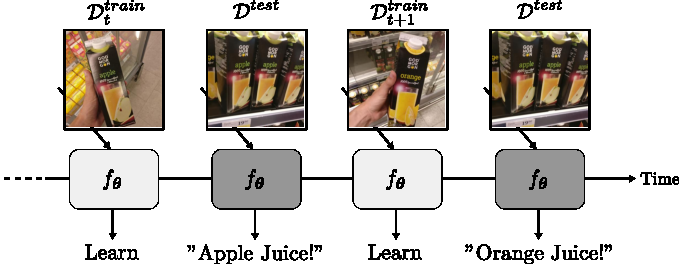
\includegraphics[width=0.8\textwidth]{Chapter4/imgs/cf_new.pdf}
	\caption{Illustration of catastrophic forgetting in a continual learning scenario. The network $f_{\vtheta}$ receives a task dataset of an Apple Juice class in $\gD_{t}^{train}$ to learn, and correctly predicts the Apple Juice class in the unseen test image in $\gD^{test}$. The next task dataset involves learning an Orange Juice class from $\gD_{t+1}^{train}$ which $f_{\vtheta}$ adapts to without retaining knowledge about the Apple Juice class, such that $f_{\vtheta}$ makes the wrong prediction during evaluation on $\gD^{test}$ again. }
	\vspace{-2mm}
	\label{fig:catastrophic_forgetting_example}
\end{figure}


\section{Related Work}\label{chap4:sec:related_work}

In this section, we give an overview of different approaches in CL, especially replay-based methods which our proposed replay scheduling approach in Paper \ref{paperC} and \ref{paperD} is based on. 

\vspace{-3mm}
\paragraph{Continual Learning.} The existing CL approaches for mitigating catastrophic forgetting in neural networks can broadly be divided into three main areas, namely, regularization-based, architecture-based, and replay-based methods. 
Regularization-based methods mainly focus on 
preventing the parameters important for previous tasks from wide changes and fit the remaining parameters to new tasks~\cite{kirkpatrick2017overcoming, zenke2017continual, nguyen2017variational}. 
Knowledge distillation methods~\cite{hinton2015distilling} also belong to these methods where stored classification logits are used for regularizing the output units for previous tasks in the network~\cite{li2017learning, schwarz2018progress}.
More recently, projection-based approaches have been proposed for constraining the parameter updates to subspaces which avoid interference with previous tasks~\cite{saha2021gradient, kao2021natural}. 
Architecture-based methods focus on adding task-specific network modules for every seen task~\cite{rusu2016progressive, yoon2017lifelong, yoon2019scalable, ebrahimi2020adversarial}, or isolating parameters for predicting specific task in fixed-size networks~\cite{mallya2018packnet, serra2018overcoming, schwarz2021powerpropagation}. 
Replay-based methods revisits samples from old tasks when learning new tasks. The old samples are either stored in an external memory~\cite{chaudhry2019tiny, hayes2020remind, rolnick2018experience,jin2020gradient,verwimp2021rehearsal}, or synthesized with a generative model~\cite{shi2019variational, van2018generative, van2020brain, wu2018memory}. 
Both regularization- and architecture-based methods can be combined with replay for improving the models capability of remembering tasks~\cite{buzzega2020dark,douillard2020podnet,ebrahimi2020adversarial,joseph2020meta,mirzadeh2020linear,nguyen2017variational,pan2020continual,von2019continual}. 
Our replay scheduling idea is originated from replay-based methods which we will cover more in detail next. 

%\paragraph{Continual Learning.} There exist many different approaches in CL for mitigating catastrophic forgetting in neural networks. In general, these approaches can be divided into three main cores, namely, \textit{regularization-based}, \textit{architecture-based}, and \textit{replay-based} methods. Regularization-based methods are mainly focused on applying regularization techniques on parameters important for recognizing old tasks and fit the remaining parameters to new tasks~\cite{kirkpatrick2017overcoming, zenke2017continual, nguyen2017variational}. Knowledge distillation methods~\cite{hinton2015distilling} also belong to these approaches where classification logits are used for regularizing the output units for previous tasks in the network~\cite{li2017learning, schwarz2018progress}. More recently, there are some works that uses projection-based approaches for constraining the parameter updates to subspaces which avoid interference with previous tasks~\cite{saha2021gradient, kao2021natural}. Architecture-based approaches focuses on adding task-specific network modules for every seen task~\cite{rusu2016progressive, yoon2017lifelong, yoon2019scalable, ebrahimi2020adversarial}, or isolating parameters for predicting specific task in fixed-size networks~\cite{mallya2018packnet, serra2018overcoming, schwarz2021powerpropagation}. Replay-based methods re-trains on samples of old tasks when learning new tasks. The old samples are either stored in an external memory~\cite{chaudhry2019tiny, hayes2020remind, rolnick2018experience}, or synthesized with a generative model~\cite{shi2019variational, van2018generative, van2020brain, wu2018memory}. Both regularization- and architecture-based methods can be combined with replay for improving the models capability of remembering tasks [Add REFs]. Our replay scheduling idea is originated from replay-based methods which we will cover more in detail next. 

\vspace{-3mm}
\paragraph{Replay-based Continual Learning.} 
Much research effort in replay-based CL has focused on selecting higher quality samples to store in memory~\cite{aljundi2019gradient, borsos2020coresets, chaudhry2019tiny, chrysakis2020online, hayes2019memory, isele2018selective, lopez2017gradient, nguyen2017variational, rebuffi2017icarl, yoon2021online}. In \cite{chaudhry2019tiny}, several selection strategies are reviewed in scenarios with tiny memory capacity, such as reservoir sampling~\cite{vitter1985random}, first-in first-out buffer~\cite{lopez2017gradient}, k-Means, and Mean-of-Features~\cite{rebuffi2017icarl}. However, elaborate selection strategies have been shown to give little benefit over random selection for image classification problems~\cite{chaudhry2018riemannian, hayes2020remind}. 
More recent work has been focused on enhancing the memory capacity by storing compressed features rather than raw data~\cite{hayes2020remind, iscen2020memory, pellegrini2019latent}, evolving the memory samples using data augmentation to avoid overfitting~\cite{jin2020gradient,bang2021rainbow}, and using contrastive learning to improve memory retention~\cite{cha2021co2l,mai2021supervised}. 
Selecting the time to replay old tasks has mostly been ignored in the literature, with an exception in~\cite{aljundi2019online} which replays memory samples that would most interfere with a foreseen parameter update. Our replay scheduling approach differs from the above mentioned works since we focus on learning to select which tasks to replay. Nevertheless, our scheduling can be combined with any selection strategy and replay-based method.


%\paragraph{Replay-based Continual Learning.} In this thesis, we focus on replay-based methods with external memories for storing historical data. The most common selection strategy for filling the memory is random sampling from the used datasets. There exist several works focusing on selecting high quality samples for storing in the memory [Add REFs]. However, in image classification problems, random sampling has been shown to often perform on par with more elaborate selection strategies~\cite{chaudhry2018riemannian, hayes2020remind}. In contrast to using various memory selection methods, there has been proposals of retrieval policies over which samples to select for replay from the memory, for instance, selecting the samples that will mostly interfere with the parameter update with batches of new data~\cite{aljundi2019online}. Our replay scheduling approach differs from this method as we focus on selecting which tasks to select for replay rather than the individual samples to retrieve from the memory. More recent works have focused on evolving the memory samples through data augmentation to avoid overfitting to the memory [Add REFs], and also by using contrastive learning to improve discriminating between tasks. Another direction has been to increasing the storage capacity to store more samples by compressing raw data into features that are more memory-cheap [Add REFs]. The above mentioned methods assume that the memory is small and allocates equal storage amount for all tasks. Our new problem setting for memory-based CL is different from this assumption as we argue that data storage is cheap in many real-world applications. Hence, we compose a replay memory with data from historical tasks before learning new tasks because the amount of compute is limited. However, replay scheduling can be combined with of the mentioned methods as it only differs with the standard memory-based CL setting in that the replay memory has to be selected at every new task. 

%\vspace{-3mm}
%\paragraph{Generalization in Reinforcement Learning.} Generalization in RL is an active research field where much focus has been put on developing proper benchmark datasets for evaluating generalization capabilities of RL agents~\cite{cobbe2019quantifying, cobbe2020leveraging, nichol2018gotta, yu2020meta}.  Regularization techniques from supervised learning have been used to investigate whether these can enhance generalization in RL~\cite{cobbe2019quantifying, farebrother2018generalization, igl2019generalization}, and also how variations in the environments help to obtain agents that generalize better~\cite{packer2018assessing, zhang2018dissection}. Algorithms for enabling fast adaptation to new environments, such as new tasks~\cite{finn2017model, kessler2021same} and new action spaces~\cite{chandak2019learning, jain2020generalization}, has also been studied. The survey by Kirk \etal~\cite{kirk2021survey} focuses on zero-shot policy transfer where the policy must generalize to unseen dynamics in the test environments as additional queries could be disallowed in real-world scenarios~\cite{yang2019single, ball2021augmented}. In Paper \ref{paperD}, we consider using RL for learning policies for scheduling which tasks to replay in CL settings to mitigate catastrophic forgetting in the classifier. The policy is trained using experiences from multiple CL environments and then tested in new CL environments with unseen dynamics such as new task orders and datasets. 
%We evaluate our learned policies on the zero-shot policy transfer setting where the goal is to mitigate catastrophic forgetting in new CL scenarios. The rewards are accessible through accuracies calculated on validation datasets, however, fine-tuning the policy during CL training is prohibited.  



% General CL papers, add new papers that you have seen. Then Replay/memory-based CL approaches, add new and contrastive approaches. Perhaps something on meta-policy learning approaches, would be useful to tell how we use reinforcement learning here

%TO-DO \MK{A short and cozy table fo this, similar to survey by Delange etal 2021}
%\paragraph{Similarities and Differences between Continual Learning and other fields.} \MK{A short and cozy table fo this, similar to survey by Delange etal 2021}


\section{Replay Scheduling in Continual Learning}\label{chap4:sec:replay_scheduling_in_cl}

In this section, we present our proposed replay scheduling approach studied in Paper \ref{paperC} and \ref{paperD} for mitigating catastrophic forgetting in CL. 
More specifically, we focus on the contributions in Paper \ref{paperC}, where we introduce a slightly new CL setting that considers real-world needs where all historical data can be available since data storage is cheap. Additionally, we demonstrate the advantages of replay scheduling in such setting where we select which tasks to replay, where we use Monte Carlo tree search (MCTS)~\cite{coulom2006efficient} to search for efficient replay schedules by allowing multiple episodes in single CL environments. 


%In this section, we introduce a slightly new CL setting considering the real-world needs where all historical data can be available since data storage is cheap. However, the amount of compute is limited when the model is updated on new data due to operational costs. Hence, it is impossible for the model to leverage from all the available historical data to mitigate catastrophic forgetting. The goal then becomes to learn how we can select subsets of historical data for replay to efficiently reduce forgetting of the old tasks. We will refer to these subsets of historical data as the \textit{replay memory} throughout this chapter. The size of the replay memory affects the processing time when learning new tasks as well as the allowed time for the training phase. When composing the replay memory, we focus on determining the number of samples to draw from the seen tasks in the historical data rather than selecting single stored instances. Next, we introduce the problem setting in more detail as well as the notation of the new CL setting. 


\subsection{New Problem Setting for Continual Learning}

In this section, we describe the proposed CL setting presented in Paper \ref{paperC}. We assume that historical data is accessible at any time for mitigating catastrophic forgetting in the model. However, re-training the model on all available historical data is prohibited due to limitations on compute and data transmission times. Therefore, the goal is to determine which historical tasks to replay and sample a small replay memory from the selected tasks to mitigate catastrophic forgetting as efficiently as possible. 

The notation of this problem setting resembles the traditional CL setting for image classification. We let a neural network $f_{\vphi}$, parameterized by $\vphi$, learn $T$ tasks from the datasets $\gD_1, \dots, \gD_T$ arriving sequentially one at a time. The $t$-th dataset $\gD_t = \{(\vx_{t}^{(i)}, y_{t}^{(i)})\}_{i=1}^{N_{t}}$ consists of $N_t$ samples where $\vx_{t}^{(i)}$ and $y_{t}^{(i)}$ are the $i$-th data point and class label respectively. Additionally, the dataset is split into training, validation, and test sets such that $\gD_{1:T} = \{(\gD_{t}^{train}, \gD_{t}^{val}, \gD_{t}^{test})\}_{t=1}^{T}$. The training objective at task $t$ is given by 
%\vspace{-2mm}
\begin{align}
	\underset{\vphi}{\text{min}} \sum_{i=1}^{N_t} \gL(f_{\vphi}(\vx_t^{(i)}), y_{t}^{(i)}),
\end{align}
where $\gL(\cdot)$ is the loss function, which in our case is the cross-entropy loss. The challenge is for the network $f_{\vphi}$ to retain its classification performance on the previous $t-1$ tasks. 

We assume that historical data from old tasks are accessible at any time step. However, we can only fill a small replay memory $\gM$ with $M$ historical samples for mitigating catastrophic forgetting of old tasks due to processing time constraints. The challenge then becomes how to select the $M$ samples from the historical data to include in the replay memory that efficiently retain the previous knowledge. 
We focus on selecting the samples on task-level by deciding on the task proportions $(p_1, \dots, p_{t-1})$ on samples to fetch from each task, where $\sum_{i=1}^{t-1} p_i = 1$ and $p_{i} \geq 0$. The number of samples from task $i$ to place in $\gM$ is given by $p_i \cdot M$. To simplify the selection of which tasks to replay, we construct a finite set of possible task proportions that can be used for constructing $\gM$. 

This problem setting shares several assumptions with traditional CL, such as:
\begin{itemize}[noitemsep,topsep=1pt]
	\item The model receives the datasets at different time steps from a continuous stream.
	\item Re-training on all historical data is prohibited.
	\item The model should perform well overall across all seen tasks and, hence, mitigate catastrophic forgetting.
	\item Replay memory size $M$ is small.
\end{itemize}
The only difference with this setting and traditional CL is that all historical has been stored rather than deleted, and we can access this data to fill the replay memory $\gM$ to mitigate catastrophic forgetting. We argue that this setting aligns well with real-world needs as data storage is cheap and easy to maintain but retraining large machine learning models is computationally expensive. Therefore, we use small replay memory sizes to limit the processing times of replay when the model is learning new tasks. 


%\paragraph{Comparison to Traditional CL.} The new setting has several similarities to the traditional CL setting. Both settings share the fundamental setting that the data arrive in streams and re-training on all historical data is prohibited. Also, the goal that the model should perform well both historical tasks and tasks associated with new data remains the same. In replay-based CL, we also share the same constraints that the memory size is limited. However, we argue that this limitation is mainly associated with compute rather than of storage. Our assumption aligns with the real-world where data storage is cheap and easy to maintain, but retraining large machine learning models is computationally expensive. The only difference is that we allow filling the limited replay memory from historical data or some other external memory. Here, we argue that historical data is stored rather than deleted in many real-world settings~\cite{bailis2017macrobase}. Thus, we should keep the limited memory assumption for training but allow access to historical data to fill the replay memory to make CL align with real-world needs.
%\MK{TO-DO: this paragraph can be written in a more humble way, more like "this is something worth to investigate"}



%\subsection{Replay Scheduling for Mitigating Catastrophic Forgetting}
\subsection{Monte Carlo Tree Search for Replay Scheduling}

In this section, we describe how we used MCTS in Paper \ref{paperC} to show the advantages of replay scheduling in the new CL setting. We focus on an ideal CL environment where executing multiple episodes is allowed to enable searching for replay schedules. For demonstration purposes, we use MCTS for finding replay schedules that efficiently mitigate catastrophic forgetting by selecting compositions of replay memories at different time steps. 

\begin{wrapfigure}{r}{0.43\textwidth}
\hspace{-4mm}
\begin{minipage}{0.43\textwidth}
\vspace{-7mm}
\begin{algorithm}[H]
	\footnotesize
	\caption{Discretization of action space with task proportions}
	\label{alg:action_space_discretization}
	\begin{algorithmic}[1]
		\Require Number of tasks $T$
		\State $\gT = ()$ %\Comment{Initialize sequence for storing actions}
		\For{$i = 1, \dots, T-1$}
		\State $\gP_i = \{\}$ %\Comment{Set for storing task proportions at $i$}
		\State $\gB = \texttt{combinations}([1:i], i)$ %\Comment{Get bin vectors of size $i$ with bins $1, ..., i$}
		\State $\gB^{*} = \texttt{unique}(\texttt{sort}(\gB))$ %\Comment{Only keep unique bin vectors}
		\For{$\vb_i \in \gB^{*}$}
		\State $\vp_i = \texttt{bincount}(\vb_i) / i$ %\Comment{Calculate task proportion}
		\State $\gP_i = \gP_i \cup \{ \vp_i \}$ %\Comment{Add task proportion to set}
		\EndFor
		\State $\gT[i] = \gP_i$ %\Comment{Add set of task proportions to action sequence}
		\EndFor
		\State \Return $\gT$ %\Comment{Return action sequence as discrete action space}
	\end{algorithmic}
\end{algorithm}
\end{minipage}
\end{wrapfigure}
We define a replay schedule as a sequence $S = (\vp_1, \dots, \vp_{T-1})$, where $\vp_i = (p_1, \dots, p_{T-1})$ for $1 \leq i \leq T-1$ is the sequence of task proportions for determining how many samples per task to fill the replay memory with at time step $i$. 
To make the selection of task proportions tractable, we construct a discrete action space with a finite number of choices for how to construct the replay memory at different time steps. Algorithm \ref{alg:action_space_discretization} shows the procedure for creating this action space. At task $i$, we have $i-1$ historical tasks that we can choose from. We then generate all possible bin vectors $\vb_i = [b_1, \dots, b_{i}] \in \gB_i$ of size $i$ where each element are a task index $1, ..., i$. The elements in each bin vector are sorted by task index, and we only keep the unique bin vectors after sorting. For example, at $i=2$, the unique choices of vectors are $[1,1], [1,2], [2,2]$, where $[1,1]$ indicates that all samples in the replay memory should be from task 1, $[1,2]$ indicates that half memory is from task 1 and the other half are from task etc. 
The task proportions are then computed by counting the number of occurrences of each task index in $\vb_i$ and dividing by $i$, such that $\vp_i = \texttt{bincount}(\vb_i) / (i)$. From this specification, we have built a tree $\gT$ with different task proportions that can be selected at different time steps. A replay schedule $S$ is constructed by traversing through $\gT$ and appending a single task proportion from every task level to $S$.  


The tree-shaped action space of task proportions grows fast with the number of tasks, which complicates studying replay scheduling in datasets with longer task-horizons. 
Therefore, we proposed using MCTS since it has been successful in applications with large action spaces~\cite{browne2012survey, chaudhry2018feature, silver2016mastering}. In our case, MCTS concentrates the search for replay schedules in directions with promising CL performance in the environment. 
Each memory composition in the action space corresponds to a node that can be visited by MCTS. For instance, at task $t$, the node $v_t$ is related to a task proportions $\vp_{t}$ that can be used for retrieving a replay memory from the historical data. 
We store the related task proportion $\vp_t$ from every visited node $v_t$ in the replay schedule $S$. The final replay schedule is then used for constructing the replay memories at each task during the CL training. 
Figure \ref{fig:mcts_outline} shows an illustration of the procedure for executing MCTS to search for replay schedules, where each step involves the following:

\begin{figure}[t]
	\centering
	
\tikzstyle{block} = [rectangle, draw, %text width=4em, 
text centered, rounded corners, 
minimum width=6em,
minimum height=2em, node distance=3cm]
\tikzstyle{textblock} = [rectangle, text width=8em, 
text centered, font=\footnotesize\sffamily]
%minimum width=6em,
%minimum height=2em]
\tikzstyle{line} = [draw, -latex, very thick]
\tikzstyle{treenode} = [circle, draw, inner sep=2pt]
\tikzstyle{triangle} = [regular polygon,regular polygon sides=3, draw, inner sep=2pt]

\colorlet{myorange}{green!10!orange!90!}
\definecolor{midnightblue}{rgb}{0.1, 0.1, 0.44}
\definecolor{royalblue}{rgb}{0.25, 0.41, 0.88}

\begin{tikzpicture}[font=\small\sffamily]
	% Place nodes
	\node [block] (selection) {Selection}; 
	\node [block, right of=selection] (expansion) {Expansion};
	\node [block, right of=expansion] (simulation) {Simulation};
	\node [block, right of=simulation] (backprop) {Backpropagation};
	\node [rectangle, text centered, above of=expansion, xshift=4em, yshift=-0.8em] (repeat) {Repeat X times};
	\node [textblock, below of=selection, yshift=-6em] (test) {Execute tree policy until a leaf node at task $t$ is reached};
	\node [textblock, below of=expansion, yshift=-6em] (test) {Create new node in tree at task $t+1$};
	\node [textblock, below of=backprop, yshift=-6.5em] (test) {The result from replay schedule is backpropagated through the tree};
	% Draw edges
	\path [line] (selection) -- (expansion);
	\path [line] (expansion) -- (simulation);
	\path [line] (simulation) -- (backprop);
	\path [line] (repeat.west) -- ($(repeat.west) - (13.3em,0)$) |- (selection.west);
	\path [line, -] (backprop.east) -- ($(backprop.east) + (0.5em,0)$) |- (repeat.east);
	
	% Place trees
	% Selection tree
	\node [treenode, below of=selection, very thick, royalblue, yshift=1em] {} [sibling distance=1.5em, level distance=1.5em] {} 
	child[very thick, royalblue, ->] { node [treenode] {}
		child[thin, black, -] { node [treenode] {} }
		child[very thick, royalblue] { node [treenode] {}
		}
	}
	child { node [treenode] {}}
	child { node [treenode] {}
		child { node [treenode] {}}
		child { node [treenode] {}}
	};
	% Expansion tree
	\node [treenode, below of=expansion, yshift=1em] {} [sibling distance=1.5em, level distance=1.5em] {} 
	child[] { node [treenode] {}
		child[] { node [treenode] {}}
		child[] { node [treenode, very thick, royalblue] {}
			child[very thick, royalblue, ->] { node [treenode] {}} }}
	child { node [treenode] {}}
	child { node [treenode] {}
		child { node [treenode] {}}
		child { node [treenode] {}}};
	% Simulation tree
	\node [treenode, below of=simulation, yshift=1em] {} [sibling distance=1.5em, level distance=1.5em] {} 
	child[] { node [treenode] {}
		child[] { node [treenode] {}}
		child[] { node [treenode] {}
			child[] { node [treenode, very thick, royalblue] {}
				child[very thick, dashed, royalblue, ->] { node [triangle, yshift=-3em, solid] {} edge from parent node [right, black, text width=5em, font=\footnotesize\sffamily, xshift=0.4em] {Simulation until task $T$ is reached}}
			} 
		}
	}
	child { node [treenode] {}}
	child { node [treenode] {}
		child { node [treenode] {}}
		child { node [treenode] {}}};
	% Backprop tree    
	\node [treenode, below of=backprop, very thick, myorange, yshift=1em] {} [sibling distance=1.5em, level distance=1.5em] {} 
	child[very thick, myorange, <-]  { node [treenode] {}
		child[thin, black, -] { node [treenode] {}}
		child[very thick, myorange, <-]  { node [treenode] {}
			child[very thick, myorange, <-] { node [treenode] {}} }}
	child { node [treenode] {}}
	child { node [treenode] {}
		child { node [treenode] {}}
		child { node [treenode] {}}
	};
	
\end{tikzpicture}
	\caption{Outline of MCTS when searching for replay schedules. }
	\label{fig:mcts_outline}
	\vspace{-2mm}
\end{figure}

\begin{itemize}[topsep=1pt, itemsep=1pt, label={}, leftmargin=*]
	\item {\bf Selection.} During a rollout, the tree policy either selects an unvisited child randomly from the current node $v_t$, or selects the next node by evaluating the Upper Confidence Tree (UCT)~\cite{kocsis2006bandit} if all children has been visited earlier.
	The child $v_{t+1}$ with the highest UCT score is selected using the function from \cite{chaudhry2018feature}:
	\begin{align}\label{eq:uct}
		UCT(v_t, v_{t+1}) = \text{max}(q(v_{t+1})) + C \sqrt{\frac{2 \log(n(v_{t}))}{n(v_{t+1})}},
	\end{align}
	where $q(\cdot)$ is the reward function, $C$ the exploration constant, and $n(\cdot)$ the number of node visits. The tree policy is executed until a leaf node $v_t$ is reached.
	
	\item {\bf Expansion.} If the leaf node $v_t$ has unvisited children, the search tree is expanded with one of the unvisited child nodes $v_{t+1}$ selected with uniform sampling. 
	
	\item {\bf Simulation and Reward.} After the expansion step, the succeeding nodes are selected randomly until reaching a terminal node $v_T$. The task proportions $\vp_{1:T-1}$ from the visited nodes in the rollout constitutes the replay schedule $S$. After training the network using $S$ for replay, we calculate the reward for the rollout given by $r = \frac{1}{T} \sum_{i=1}^T A_{T, i}^{(val)}$, where $A_{T, i}^{(val)}$ is the validation accuracy of task $i$ at task $T$.  
	
	\item {\bf Backpropagation.} The reward $r$ is backpropagated from the expanded node $v_{t+1}$ to the root node, where the reward function $q(\cdot)$ and number of visits $n(\cdot)$ are updated at each node in the path. 
\end{itemize}
As mentioned earlier, we use MCTS to search for replay schedules to illustrate the importance of learning the time to learn. To this end, we study replay scheduling in an ideal CL environment where multiple episodes is allowed to find replay schedules. However, in the standard CL setting, multiple episodes are prohibited which currently prevents replay scheduling to be applied in real-world CL scenarios. In the next section, we present a policy learning framework based on RL to learn replay scheduling policies that generalize. 


%\section{Meta Policy Learning for Replay Scheduling}\label{sec:meta_policy_learning_for_replay_scheduling}
\section{Policy Learning for Replay Scheduling}\label{chap4:sec:policy_learning_for_replay_scheduling}

In this section, we introduce the RL-based framework for learning replay scheduling policies that was proposed in Paper \ref{paperD}. In real-world CL settings, learning the policy with multiple episodes is infeasible, which is why we need a general policy for replay scheduling.
Our intuition is that there may exist general patterns regarding the replay scheduling, e.g., tasks that are harder or have been forgotten should be replayed more often. Moreover, the policy may non-trivially take task properties into consideration. Therefore, we aim to learn policies that select which tasks to replay from states representing the current task performance in the CL environments. The policy can then be applied for mitigating catastrophic forgetting in new CL scenarios. 

We model the CL environments as Markov Decision Processes~\cite{bellman1957markovian} (MDPs) where each MDP is represented as a tuple $E_i = (\gS_i, \gA, P_i, R_i, \mu_i, \gamma)$ consisting of the state space $\gS_i$, action space $\gA$, state transition probability $P_i(s' | s, a)$, reward function $R_i(s, a)$, initial state distribution $\mu_i(s_1)$, and discount factor $\gamma$.
We assume that we have access to a fixed set of training environments $\gE^{(train)} = \{E_1, \dots, E_K\}$ sampled from a distribution of CL environments, i.e., $E_i \sim p(E)$ for $i=1, ..., K$. 
Each environment $E_i$ contains of a network $f_{\vphi}$ and $T$ datasets $\gD_{1:T}$ where the $t$-th dataset is learned by $f_{\vphi}$ at time step $t$. Note that we will use task and time step interchangeably. 
To generate diverse CL environments, we obtain environments with different initializations of the network $f_{\vphi}$ and shuffled task orders in the dataset when we sample environments from $p(E)$. 

We define the state $s_t$ of the environment as the validation accuracies $A_{t, 1:t}^{(val)}$ on each seen task $1, ..., t$ from $f_{\vphi}$ at task $t$, i.e., $s_t = [A_{t, 1}, ..., A_{t, t}, 0, ..., 0]$, where we use zero-padding on future tasks. The action space $\gA$ is constructed as described in Algorithm \ref{alg:action_space_discretization} (Section \ref{chap4:sec:replay_scheduling_in_cl}), such that the $a_t \in \gA$ corresponds to a task proportion $\vp_t$ used for sampling the replay memory $\gM_t$. We use a dense reward based on the average validation accuracies at task $t$, i.e., $r_{t} = \frac{1}{t}\sum_{i=1}^{t} A_{t, i}^{(val)}$. The state transition distribution $P_i(s' | s, a)$ represents the dynamics of the environment, which depend on the initialization of $f_{\vphi}$ and also the task order in the dataset. More specifically, the dynamics represent how the validation accuracies varies after $f_{\vphi}$ replays according to the action $a_t$ when learning the current task. 

The procedure for training the policy goes as follows: 
The state $s_t$ is obtained by evaluating the network $f_{\vphi}$ on the validation sets $\gD_{1:t}^{(val)}$ after learning the $t$-th task from $\gD_t^{(train)}$. Action $a_t$ is selected under the policy $\pi_{\vtheta}(a | s_t)$ parameterized by $\vtheta$. The action is converted into task proportion $\vp_t$ that is used for sampling the replay memory $\gM_t$ from the historical datasets. 
We then train classifier $f_{\vphi}$ with $\gD_{t+1}^{(train)}$ and $\gM_t$, and obtain the reward $r_{t+1}$ and the next state $s_{t+1}$ by evaluating $f_{\vphi}$ on the validation sets $\gD_{1:t+1}^{(val)}$. The collected transitions $(s_t, a_t, r_{t+1}, s_{t+1})$ are used for updating the policy.  A new episode starts after $f_{\vphi}$ has learned the final task $T$. 

We evaluate the learned policy by applying it to mitigate catastrophic forgetting in new CL environments at test time. To foster generalization across environments, we train the policy on multiple environments with different dynamics, such as task orders and datasets, to learn from a diverse set of training data. The goal for the agent is to maximize the sum of rewards in each training environment. 
At test time, the policy is applied on new CL classifiers and datasets in the test environments without added computational cost nor experience collection. In Section \ref{chap4:sec:experiments}, we test the policies generalization capability to new CL environments where the task orders and datasets are unseen during training.


%In this section, we present an RL-based framework to learn policies for selecting which tasks to replay in CL scenarios. We are interested in learning such policy that can be transferred to new CL scenarios, such as new task orders and new datasets, without any additional computational cost for updating on the new domain. We take a meta-learning approach where the policy learns from episodes of experience collected from training a classifier in CL settings. The experience from the environment is represented as the classification performance on each seen task in the dataset. The policy receives the task performances for basing its action on which task that needs to be replayed at the next time step. Our goal is to obtain a policy that can generalize to be used for replay scheduling in new CL scenarios to mitigate catastrophic forgetting. Next, we describe in more detail how the framework for learning this policy works.

%By learning from gathering experience, the policy learns better for the future on how to select the tasks to replay. However, as 

%\MK{Is this how it should be motivated?}
%Imagine the scenario that we can collect experiences from many users applying their phone to CL scenarios for learning different objects to recognize sequentially. Assume that we can store the collected data (limitation here is privacy!), the models will suffer from catastrophic forgetting as they are trained in CL scenario. But we can then use the collected data to train a replay scheduling policy. The learned policy can then be transferred to new users using their phone in CL settings and the policy is used for mitigating catastrophic forgetting in their environment without additional computational cost. 

%Limitations here are of course that we potentially need lots of data for learning a policy that generalizes. Additionally, we need lots of training time and hyperparameter tuning as we are dealing with RL. Also, we need to store the data somewhere which is cheap, but it must be secure due to privacy concerns. An alternative there could be to store features instead of raw data, which is not completely flawless (I think that it's possible to revert features back to the real data to some extent) but at least it is a safer alternative. Another option for the data needed can be to gather experience from simulated environments and benchmark datasets. As the policy only takes in states with task performances, we can make use mixes of benchmark datasets and data from real contributing users. 

\begin{comment}
	
\subsection{Problem Setting}

We consider the setting where an agent selects replay schedules to mitigate catastrophic forgetting in a classifier trained in the CL setting. The environment that the agent interacts with contains a network $f_{\vphi}$ and a dataset $\gD_{1:T}$ of $T$ tasks that $f_{\vphi}$ should learn in sequential order. The dataset is split into training, validation, and test sets as $\gD_{1:T} = \{\gD_{1:T}^{\train}, \gD_{1:T}^{\val}, \gD_{1:T}^{\test}\}$ respectively. The training sets $\gD_{1:T}^{\train}$ are for the network to learn all $T$ tasks sequentially, while the $\gD_{1:T}^{\val}$ are for evaluating how well the network performs on each task during training. The task performances on the validation sets can be used for dense rewards to the RL agent. The test sets are for final evaluation and are unseen during training as standard practice to avoid overfitting.  

We consider having a distribution $p(E)$ of Markov Decision Process~\cite{bellman1957markovian} (MDP) where the MDP is represented as a tuple $E_i = (\gS_i, \gA, P_i, R_i, \mu_i, \gamma)$ consisting of the state space $\gS_i$, action space $\gA$, state transition probability $P_i(s' | s, a)$, reward function $R_i(s, a)$, initial state distribution $\mu_i(s_0)$, and discount factor $\gamma$. For training, we assume that we have access to a fixed set of training environments $\gE_{\train} = \{E_1, \dots, E_K\}$, where $E_i \sim p(E)$ for $i=1, ..., K$. Each environment $E_i$ contains of a network $f_{\vphi}$ and $T$ datasets $\gD_{1:T}$ where the $t$-th dataset is learned at time step $t$. We let the dynamics of the environments depend on the network initialization and the task order of the datasets. The states $s$ are given by the validation performance on each task from $f_{\vphi}$ which can be accuracies. Hence, the state space $\gS_i$ depends on the parameter initialization for $\vphi$. Regarding the datasets, we allow the task orders in the datasets $\gD_{1:T}$ to be shuffled for each sampled environment $E_i \sim p(E)$. Therefore, the state space is also affected by the task order as this can yield different CL performances. We assume that the action space is the same for every environment as the agent will interact with each training environment in $\gE_{\train}$. 

The goal for the agent is to maximize the accumulated returns in each training environment. The reward is given by the CL performance. We assume that we have a dense reward that we can compute from the validation sets at each time step $t$. We are therefore after a policy that works well on all environments. The intention for learning such policy is that it should generalize across environments of new CL settings, such as new task orders and datasets. As we are not allowed to go back in time in CL, we are not allowed to query the testing environments during the transfer. Hence we must apply the policy in a zero-shot setting where tuning the policy on the testing environment is prohibited.


\subsection{Deep Q-Networks for Learning Replay Scheduling Policy}

We employ DQNs for learning the policy for replay scheduling. The architecture takes states as input and outputs action values for the valid actions at the current time step $t$. We define the states $s$ as a vector with the validation performance of every seen task, where we use the validation accuracy to represent the task performance. We use zero-padding on the vector elements in the states that represent the performance for future tasks. The states can also be represented by other performance metrics, for example, the accuracy difference between time steps or forgetting measures such as backward transfer~\cite{lopez2017gradient} (BWT). For the actions, we use the discrete action space built using Algorithm \ref{alg:action_space_discretization} such that the action space $\gA_t$ is time-dependent and grows per seen task. To handle the growing action space, we assume that we know the total number of actions such that the DQN can use a fixed output layer. Therefore, we use action masking on the predicted action values to prevent the DQN from selecting invalid actions. 

\begin{algorithm}[t]
	\caption{Learning replay scheduling policy with DQN}
	\label{alg:learning_replay_scheduling_policy_with_dqn}
	\begin{algorithmic}[1]
		\Require $\gE_{\train}$: Training environments
		\Require $\vtheta$: DQN parameters
		\State $\gB = \{\}$ \Comment{Initialize replay buffer}
		\For{$i = 1, \dots, n_{\text{episodes}}$}
		\State $s_1^{i} \sim \mu_i \, \forall E_i \in \gE_{\train}$ \Comment{Get initial states}
		\For{$t=1, \dots, T-1$}
		\For{$E_i \in \gE_{\train}$}
		\State $a_t^{i} = \argmax_{a' \in \gA_t} Q_{\vtheta}(s_t^{i}, a')$ \Comment{Get actions from states}
		\State $r_t^{i}, s_{t+1}^{i} = \texttt{CLStep}(t, a_t^{i}, E_i)$
		\State $\gB = \gB \cup \{(s_{t}^{i}, a_{t}^{i}, r_{t}^{i}, s_{t+1}^{i})\}$ \Comment{Store transition in buffer}
		\State $(s_j, a_j, r_j, s_{j+1}) \stackrel{B}{\sim} \gB$ \Comment{Get mini-batch of $B$ samples from buffer}					
		%\State $\{(s_t^{(j)}, a_t^{(j)}, r_t^{(j)}, s_{t+1}^{(j)})\}_{j=1}^{B} \stackrel{B}{\sim} \gB$
		\State $\vtheta \leftarrow \vtheta - \eta \nabla_{\vtheta} (r_t + \max_{a'} Q_{\vtheta^{-}}(s_{j+1}, a') - Q_{\vtheta}(s_j, a_j))$ \Comment{Update DQN}
		\EndFor
		\EndFor 
		\EndFor
		\State \Return $\vtheta$ \Comment{Return DQN}
		
		\Statex
		
		\Function{\texttt{CLStep}}{$t$, $a_{t}$, $E$}
		\State $\gM_t \leftarrow \texttt{SampleMemory}(a_t)$ \Comment{Sample historical data from action}
		\State $f_{\vphi}^{E} \leftarrow \texttt{Train}(f_{\vphi}^{E}, \gD_{t+1}^{\train}, \gM_t)$ \Comment{Train network on current task with replay}
		\State $r_t \leftarrow \frac{1}{t+1} \sum_{i=1}^{t+1} A_{i}^{\val}$ \Comment{Compute reward from validation datasets}
		\State $s_{t+1} \leftarrow \texttt{GetState}(f_{\vphi}^{E}, \gD_{1:t+1}^{\val})$ \Comment{Get next state from validation performance}
		\State \Return $r_t$, $s_{t+1}$ \Comment{Return reward and next state}
		\EndFunction
	\end{algorithmic}
\end{algorithm}

We outline the procedure for training the DQN on multiple CL environments in Algorithm \ref{alg:learning_replay_scheduling_policy_with_dqn}. The main idea to obtain a policy that generalize is to train it on several environments with different dynamics for learning from more diverse training data~\cite{zhang2018dissection}. We let the DQN store transitions $(s_{t}^{i}, a_{t}^{i}, r_{t}^{i}, s_{t+1}^{i})$ from all environments in the same experience replay buffer $\gB$ to use for training the network. The first step is to receive the intial state $s_1$ for all environments by training the network $f_{\vphi}$ on the first dataset $\gD_1^{\train}$ in each environment, such that $s_{1}^{i} = [A_{1,1}^{\val}, 0, ..., 0]$. The DQN then selects the action $a_t$ for the current environment from the input state or selects a random action with probability $\epsilon$. The agent retrieves the reward and next state by training the environment-specific network $f_{\vphi}^{i}$ on the current task $t$ in \texttt{CLStep}. Before training starts, the action $a_{t}^{i}$ is used for sampling the replay memory $\gM_t$ using the task proportions $(\vp_1, \dots, \vp_{T-1})$ translated from $a_{t}^{i}$. The replay memory is then used for mitigating catastrophic forgetting when training on the current task. After training, the agent obtains the reward from the reward function 
\begin{align}
	R(s, a) = \frac{1}{t} \sum_{i=1}^{t} A_{t, i}^{\val},
\end{align}
where $A_{t, i}^{\val}$ is the validation accuracy on task $i$ after $f_{\vphi}$ has learned task $t$. The next state is also obtained by utilizing the validation accuracies up to task $t$, such as $s_{t+1}^{i} = [A_{t, 1}^{\val}, ..., A_{t, t}^{\val}, 0, ..., 0] \in [0, 1]^{T-1}$. The DQN is then updated by sampling a mini-batch of $B$ samples from the shared buffer $\gB$ and taking a gradient step to minimize the loss
\begin{align}
	\gL_{\text{DQN}}(\vtheta) = r_j + \max_{a'} Q_{\vtheta^{-}}(s_{j+1}, a') - Q_{\vtheta}(s_j, a_j), 
\end{align}  
where $\vtheta^{-}$ is target network which is copy of the parameters $\vtheta$ from some previous time step. By using the shared replay buffer, the DQN is trained on diverse set of environments that can generalize well to new environments with unseen dynamics from an unseen task order or a new dataset. Next, we will describe the experiments we perform to evaluate the generalization capability of the policy to new CL scenarios. 
\end{comment}


\section{Experiments}\label{chap4:sec:experiments}

In this section, we give an overview of the experimental results from Paper \ref{paperC} and \ref{paperD}. In Paper \ref{paperC}, we evaluate the benefits of replay scheduling in single CL environments using MCTS for finding replay schedules. We perform extensive evaluation to show that the replay schedules from MCTS can outperform the baselines across several CL benchmarks and different backbones. 
In Paper \ref{paperD}, we evaluate our RL-based framework using DQN~\cite{mnih2013playing} and A2C~\cite{mnih2016asynchronous} for learning policies that generalize to new CL scenarios.
We show that the learned policies can efficiently mitigate catastrophic forgetting in CL environments with new task orders and datasets that are unseen during training. 
%Full details on experimental settings and additional results are in Appendix \ref{app:experimental_settings} and \ref{app:additional_experimental_results}. Code is available as supplementary material.  

%In this section, we give an overview of the experimental results in Paper \ref{paperC} and \ref{paperD}. In Paper \ref{paperC}, we perform experiments to show that the importance of replay scheduling in our proposed problem setting for CL described in Section \ref{sec:replay_scheduling_in_cl}. We demonstrate that learning when to replay different tasks by using MCTS as an exemplar method for finding good replay schedules that are efficient in mitigating catastrophic forgetting in the classifier. In Paper \ref{paperD}, we demonstrate on benchmark datasets for CL how our RL-based framework can be used for learning replay scheduling policies. We show that our proposed method can learn policies that generalize to CL scenarios with new task orders and datasets unseen during training.  

\subsection{Results on Replay Scheduling with Monte Carlo Tree Search}

Here, we provide a selection of the experimental results from Paper \ref{paperC}. Our approach has been named Replay Scheduling MCTS (RS-MCTS). 
We evaluate the CL performance of RS-MCTS for varying memory sizes to illustrate the importance of replay scheduling. Moreover, we show that replay scheduling can benefit any replay-based method by combining scheduling with three recent CL methods, namely, HAL~\cite{chaudhry2021using}, MER~\cite{riemer2018learning}, and DER~\cite{buzzega2020dark}. Finally, we demonstrate the efficiency benefits of replay scheduling in settings when the memory size is smaller than the number of classes. We give an overview of the experimental settings, see Paper \ref{paperC} for the full experimental results and hyperparameter settings. 

\vspace{-3mm}
\paragraph{Datasets and Architectures.} We perform experiments on common CL benchmark datasets such as Split MNIST~\cite{zenke2017continual}, Split Fashion-MNIST~\cite{xiao2017fashion}, Split notMNIST~\cite{bulatov2011notMNIST}, Permuted MNIST~\cite{goodfellow2013empirical}, and Split CIFAR-100~\cite{krizhevsky2009learning, lopez2017gradient, rebuffi2017icarl} and Split miniImagenet~\cite{vinyals2016matching}. We use a 2-layer MLP with 256 hidden units and ReLU activations for Split MNIST, Split FashionMNIST, Split notMNIST, and Permuted MNIST.  For Split CIFAR-10 and CIFAR-100, we use the CNN architecture used in \cite{adel2019continual, schwarz2018progress, vinyals2016matching}, and a reduced ResNet-18 from \cite{lopez2017gradient} for Split mini-Imagenet. We use a multi-head output layer for each dataset, except Permuted MNIST where the network uses single-head output layer, such that we assume that task labels are available at test time~\cite{van2019three}. 

\vspace{-3mm}
\paragraph{Baselines.} We compare our method against the following scheduling baselines:
\begin{itemize}[itemsep=0em,topsep=1pt]
	\item {\bf Random Schedule}: Randomly select which tasks to replay.
	\item {\bf Equal Task Schedule (ETS)}: Replay all seen tasks equally.
	\item {\bf Heuristic Schedule}: Replay tasks which validation performance is below a tuned threshold found through hyperparameter searches.
\end{itemize} 

\vspace{-3mm}
\paragraph{Evaluation.} We use the following evaluation metric for measuring the CL performance
\begin{align}\label{eq:acc}
	\ACC = \frac{1}{T} \sum_{j=1}^{T} A_{T, j}^{test},
\end{align}
where $A_{T, j}^{test}$ is the accuracy of task $j$ after learning the final task $T$.  
%In Paper \ref{paperD}, we use a ranking method for comparing the ACC performance of each scheduling method within the testing environments, since the performance between environments can differ significantly when the task order changes. We then average all obtained ranking lists over the number of testing environments to obtain the ranking metric. 

\vspace{-3mm}
\begin{wrapfigure}{r}{0.50\textwidth}
	%\centering
	\vspace{-3mm}
	\hspace{-11mm}
	%\begin{minipage}{0.50\textwidth}
	\setlength{\figwidth}{0.36\textwidth}
	\setlength{\figheight}{.16\textheight}
	\resizebox{0.58\textwidth}{!}{
		


\pgfplotsset{every axis title/.append style={at={(0.5,0.80)}}} 
\pgfplotsset{every tick label/.append style={font=\tiny}}
\pgfplotsset{every major tick/.append style={major tick length=2pt}}
\pgfplotsset{every minor tick/.append style={minor tick length=1pt}}
\pgfplotsset{every axis x label/.append style={at={(0.5,-0.22)}}}
\pgfplotsset{every axis y label/.append style={at={(-0.17,0.5)}}}
´

\begin{tikzpicture}
\tikzstyle{every node}=[font=\scriptsize]
\definecolor{color0}{rgb}{0.12156862745098,0.466666666666667,0.705882352941177}
\definecolor{color1}{rgb}{1,0.498039215686275,0.0549019607843137}
\definecolor{color2}{rgb}{0.172549019607843,0.627450980392157,0.172549019607843}
\definecolor{color3}{rgb}{0.83921568627451,0.152941176470588,0.156862745098039}

\begin{groupplot}[group style={group size= 2 by 2, horizontal sep=0.7cm, vertical sep=0.8cm}]

\nextgroupplot[title=Split MNIST,
height=\figheight,
legend cell align={left},
legend columns=4,
legend style={
  nodes={scale=0.80},
  fill opacity=0.8,
  draw opacity=1,
  text opacity=1,
  at={(0.00,1.30)}, %{(3.70,-0.30)},   %{(3.72,0.13)},
  anchor=south west,
  draw=white!80!black
},
minor xtick={},
minor ytick={},
tick align=outside,
tick pos=left,
width=\figwidth,
x grid style={white!69.0196078431373!black},
xmajorgrids,
%xlabel={Memory size \(\displaystyle M\)},
xmin=0.7, xmax=7.3,
xtick style={color=black},
xtick={1,2,3,4,5,6,7},
xticklabels={8,24,80,120,200,400,800},
y grid style={white!69.0196078431373!black},
ymajorgrids,
ylabel={ACC (\%)},
ymin=0.939, ymax=0.997729043511215,
ytick style={color=black},
ytick={0.92,0.93,0.94,0.95,0.96,0.97,0.98,0.99,1},
yticklabels={92,93,94,95,96,97,98,99,100}
]
\path [fill=color0, fill opacity=0.2, line width=1pt]
(axis cs:1,0.92504620552063)
--(axis cs:1,0.981783270835876)
--(axis cs:2,0.981537520885468)
--(axis cs:3,0.988991677761078)
--(axis cs:4,0.986135482788086)
--(axis cs:5,0.991755723953247)
--(axis cs:6,0.989374697208405)
--(axis cs:7,0.994002878665924)
--(axis cs:7,0.976767957210541)
--(axis cs:7,0.976767957210541)
--(axis cs:6,0.979170620441437)
--(axis cs:5,0.964531421661377)
--(axis cs:4,0.978874921798706)
--(axis cs:3,0.979120314121246)
--(axis cs:2,0.937642157077789)
--(axis cs:1,0.92504620552063)
--cycle;

\path [fill=color1, fill opacity=0.2, line width=1pt]
(axis cs:1,0.946015386753438)
--(axis cs:1,0.970621573246562)
--(axis cs:2,0.984533286206628)
--(axis cs:3,0.988692537329328)
--(axis cs:4,0.990023216819651)
--(axis cs:5,0.990669279851693)
--(axis cs:6,0.992800317892538)
--(axis cs:7,0.994021984494329)
--(axis cs:7,0.992872175505671)
--(axis cs:7,0.992872175505671)
--(axis cs:6,0.990845362107462)
--(axis cs:5,0.986030240148307)
--(axis cs:4,0.986402863180349)
--(axis cs:3,0.980789062670673)
--(axis cs:2,0.972900553793372)
--(axis cs:1,0.946015386753438)
--cycle;

\path [fill=color2, fill opacity=0.2, line width=1pt]
(axis cs:1,0.953295697386423)
--(axis cs:1,0.969893182613577)
--(axis cs:2,0.989900327489411)
--(axis cs:3,0.987615676138068)
--(axis cs:4,0.987468694435405)
--(axis cs:5,0.987904186526891)
--(axis cs:6,0.990390603540462)
--(axis cs:7,0.991611458769248)
--(axis cs:7,0.983504221230752)
--(axis cs:7,0.983504221230752)
--(axis cs:6,0.978347876459538)
--(axis cs:5,0.975166293473109)
--(axis cs:4,0.979932985564595)
--(axis cs:3,0.979642883861932)
--(axis cs:2,0.966454952510589)
--(axis cs:1,0.953295697386423)
--cycle;

\path [fill=color3, fill opacity=0.2, line width=1pt]
(axis cs:1,0.976848125457764)
--(axis cs:1,0.986456036567688)
--(axis cs:2,0.988981068134308)
--(axis cs:3,0.992213249206543)
--(axis cs:4,0.991635799407959)
--(axis cs:5,0.991742670536041)
--(axis cs:6,0.992980241775513)
--(axis cs:7,0.994612276554108)
--(axis cs:7,0.993073880672455)
--(axis cs:7,0.993073880672455)
--(axis cs:6,0.992027640342712)
--(axis cs:5,0.990043103694916)
--(axis cs:4,0.989341855049133)
--(axis cs:3,0.989036798477173)
--(axis cs:2,0.982677280902863)
--(axis cs:1,0.976848125457764)
--cycle;

\addplot [line width=1.0pt, color0, mark=*, mark size=1, mark options={solid}]
table {%
1 0.953414738178253
2 0.959589838981628
3 0.984055995941162
4 0.982505202293396
5 0.978143572807312
6 0.984272658824921
7 0.985385417938232
};
\addlegendentry{Random}
\addplot [line width=1.0pt, color1, mark=*, mark size=1, mark options={solid}]
table {%
1 0.95831848
2 0.97871692
3 0.9847408
4 0.98821304
5 0.98834976
6 0.99182284
7 0.99344708
};\addlegendentry{ETS}
\addplot [line width=1.0pt, color2, mark=*, mark size=1, mark options={solid}]
table {%
1 0.96159444
2 0.97817764
3 0.98362928
4 0.98370084
5 0.98153524
6 0.98436924
7 0.98755784
};
\addlegendentry{Heuristic}
\addplot [line width=1.0pt, color3, mark=*, mark size=1, mark options={solid}]
table {%
1 0.981652081012726
2 0.985829174518585
3 0.990625023841858
4 0.990488827228546
5 0.990892887115479
6 0.992503941059113
7 0.993843078613281
};\addlegendentry{Ours}




%
\nextgroupplot[title=Split FashionMNIST,
height=\figheight,
legend cell align={left},
legend style={
  nodes={scale=0.7},
  fill opacity=0.8,
  draw opacity=1,
  text opacity=1,
  at={(0.48,0.03)},
  anchor=south west,
  draw=white!80!black
},
minor xtick={},
minor ytick={0.89, 0.91, 0.93, 0.95, 0.97, 0.99},
tick align=outside,
tick pos=left,
width=\figwidth,
x grid style={white!69.0196078431373!black},
xmajorgrids,
%xlabel={Memory size \(\displaystyle M\)},
xmin=0.7, xmax=7.3,
xtick style={color=black},
xtick={1,2,3,4,5,6,7},
xticklabels={8,24,80,120,200,400,800},
y grid style={white!69.0196078431373!black},
ymajorgrids,
yminorgrids,
%ylabel={ACC},
ymin=0.899,%0.891766529814355,
ymax=0.996494715797058,
ytick style={color=black},
ytick={0.88,0.9,0.92,0.94,0.96,0.98,1},
yticklabels={88, 90, 92, 94, 96, 98, 100}
]
\path [fill=color0, fill opacity=0.2, line width=1pt]
(axis cs:1,0.96419358253479)
--(axis cs:1,0.976246356964111)
--(axis cs:2,0.984048008918762)
--(axis cs:3,0.98274040222168)
--(axis cs:4,0.982234418392181)
--(axis cs:5,0.985867142677307)
--(axis cs:6,0.985980749130249)
--(axis cs:7,0.988571465015411)
--(axis cs:7,0.980668723583221)
--(axis cs:7,0.980668723583221)
--(axis cs:6,0.972739219665527)
--(axis cs:5,0.975212812423706)
--(axis cs:4,0.954325616359711)
--(axis cs:3,0.976219773292542)
--(axis cs:2,0.962551951408386)
--(axis cs:1,0.96419358253479)
--cycle;

\path [fill=color1, fill opacity=0.2, line width=1pt]
(axis cs:1,0.965724160568608)
--(axis cs:1,0.979275839431391)
--(axis cs:2,0.983843648420532)
--(axis cs:3,0.987767732323772)
--(axis cs:4,0.988072744085454)
--(axis cs:5,0.988506841180757)
--(axis cs:6,0.989178836422143)
--(axis cs:7,0.990307375485654)
--(axis cs:7,0.989052624514346)
--(axis cs:7,0.989052624514346)
--(axis cs:6,0.987461163577857)
--(axis cs:5,0.983413158819243)
--(axis cs:4,0.982567255914546)
--(axis cs:3,0.970792267676228)
--(axis cs:2,0.972876351579468)
--(axis cs:1,0.965724160568608)
--cycle;

\path [fill=color2, fill opacity=0.2, line width=1pt]
(axis cs:1,0.955000050761585)
--(axis cs:1,0.970759949238415)
--(axis cs:2,0.98603178628668)
--(axis cs:3,0.981832320290786)
--(axis cs:4,0.983967730086771)
--(axis cs:5,0.978253058795492)
--(axis cs:6,0.991734343706935)
--(axis cs:7,0.969833098095523)
--(axis cs:7,0.896526901904478)
--(axis cs:7,0.896526901904478)
--(axis cs:6,0.916425656293065)
--(axis cs:5,0.938266941204508)
--(axis cs:4,0.921192269913229)
--(axis cs:3,0.942567679709214)
--(axis cs:2,0.92920821371332)
--(axis cs:1,0.955000050761585)
--cycle;

\path [fill=color3, fill opacity=0.2, line width=1pt]
(axis cs:1,0.982129275798798)
--(axis cs:1,0.984390676021576)
--(axis cs:2,0.987218379974365)
--(axis cs:3,0.988464534282684)
--(axis cs:4,0.989360094070435)
--(axis cs:5,0.989464402198792)
--(axis cs:6,0.989146828651428)
--(axis cs:7,0.990860760211945)
--(axis cs:7,0.988419115543365)
--(axis cs:7,0.988419115543365)
--(axis cs:6,0.98689329624176)
--(axis cs:5,0.987175583839417)
--(axis cs:4,0.985639929771423)
--(axis cs:3,0.983615458011627)
--(axis cs:2,0.982341647148132)
--(axis cs:1,0.982129275798798)
--cycle;
\addplot [line width=1.0pt, color0, mark=*, mark size=1, mark options={solid}]
table {%
1 0.970219969749451
2 0.973299980163574
3 0.979480087757111
4 0.968280017375946
5 0.980539977550507
6 0.979359984397888
7 0.984620094299316
};
%\addlegendentry{Random}
\addplot [line width=1.0pt, color1, mark=*, mark size=1, mark options={solid}]
table {%
1 0.9725
2 0.97836
3 0.97928
4 0.98532
5 0.98596
6 0.98832
7 0.98968
};
%\addlegendentry{ETS}
\addplot [line width=1.0pt, color2, mark=*, mark size=1, mark options={solid}]
table {%
1 0.96288
2 0.95762
3 0.9622
4 0.95258
5 0.95826
6 0.95408
7 0.93318
};
%\addlegendentry{Heuristic}
\addplot [line width=1.0pt, color3, mark=*, mark size=1, mark options={solid}]
table {%
1 0.983259975910187
2 0.984780013561249
3 0.986039996147156
4 0.987500011920929
5 0.988319993019104
6 0.988020062446594
7 0.989639937877655
};
%\addlegendentry{Ours}



%\nextgroupplot[title=Split notMNIST,
height=\figheight,
legend cell align={left},
legend style={
  nodes={scale=0.7},
  fill opacity=0.8,
  draw opacity=1,
  text opacity=1,
  at={(0.48,0.03)},
  anchor=south west,
  draw=white!80!black
},
minor xtick={},
minor ytick={0.91, 0.93, 0.95, 0.97},
tick align=outside,
tick pos=left,
width=\figwidth,
x grid style={white!69.0196078431373!black},
xmajorgrids,
%xlabel={Memory size \(\displaystyle M\)},
xmin=0.7, xmax=7.3,
xtick style={color=black},
xtick={1,2,3,4,5,6,7},
xticklabels={8,24,80,120,200,400,800},
y grid style={white!69.0196078431373!black},
ymajorgrids,
yminorgrids,
%ylabel={ACC},
ymin=0.899, ymax=0.968037298370892,
ytick style={color=black},
ytick={0.9,0.92,0.94,0.96,0.98},
yticklabels={90, 92, 94, 96, 98}
]
\path [fill=color0, fill opacity=0.2, line width=1pt]
(axis cs:1,0.898027122020721)
--(axis cs:1,0.932646334171295)
--(axis cs:2,0.949522912502289)
--(axis cs:3,0.941804111003876)
--(axis cs:4,0.945932507514954)
--(axis cs:5,0.944690823554993)
--(axis cs:6,0.958006739616394)
--(axis cs:7,0.963123440742493)
--(axis cs:7,0.937735080718994)
--(axis cs:7,0.937735080718994)
--(axis cs:6,0.941412806510925)
--(axis cs:5,0.925552010536194)
--(axis cs:4,0.917471051216125)
--(axis cs:3,0.924349844455719)
--(axis cs:2,0.907234847545624)
--(axis cs:1,0.898027122020721)
--cycle;

\path [fill=color1, fill opacity=0.2, line width=1pt]
(axis cs:1,0.905642837956127)
--(axis cs:1,0.936302282043873)
--(axis cs:2,0.945930444061739)
--(axis cs:3,0.952986088925952)
--(axis cs:4,0.959824157530047)
--(axis cs:5,0.952829054017519)
--(axis cs:6,0.959656752670672)
--(axis cs:7,0.962564882794123)
--(axis cs:7,0.947773837205876)
--(axis cs:7,0.947773837205876)
--(axis cs:6,0.948538687329328)
--(axis cs:5,0.942894385982481)
--(axis cs:4,0.946525122469953)
--(axis cs:3,0.939538551074048)
--(axis cs:2,0.917796675938261)
--(axis cs:1,0.905642837956127)
--cycle;

\path [fill=color2, fill opacity=0.2, line width=1pt]
(axis cs:1,0.92575112968193)
--(axis cs:1,0.94785415031807)
--(axis cs:2,0.955205714329457)
--(axis cs:3,0.958007719572493)
--(axis cs:4,0.952085855254064)
--(axis cs:5,0.955086757682649)
--(axis cs:6,0.947191690371997)
--(axis cs:7,0.964993528242304)
--(axis cs:7,0.936188951757696)
--(axis cs:7,0.936188951757696)
--(axis cs:6,0.909628229628003)
--(axis cs:5,0.922580682317351)
--(axis cs:4,0.916396464745937)
--(axis cs:3,0.906849720427507)
--(axis cs:2,0.904118125670543)
--(axis cs:1,0.92575112968193)
--cycle;

\path [fill=color3, fill opacity=0.2, line width=1pt]
(axis cs:1,0.939071178436279)
--(axis cs:1,0.951526403427124)
--(axis cs:2,0.958871364593506)
--(axis cs:3,0.954144775867462)
--(axis cs:4,0.952358484268188)
--(axis cs:5,0.95714259147644)
--(axis cs:6,0.956836819648743)
--(axis cs:7,0.9615877866745)
--(axis cs:7,0.9475919008255)
--(axis cs:7,0.9475919008255)
--(axis cs:6,0.94806444644928)
--(axis cs:5,0.94659161567688)
--(axis cs:4,0.93076229095459)
--(axis cs:3,0.942625343799591)
--(axis cs:2,0.945715665817261)
--(axis cs:1,0.939071178436279)
--cycle;

\addplot [line width=1.0pt, color0, mark=*, mark size=1, mark options={solid}]
table {%
1 0.915336728096008
2 0.928378880023956
3 0.933076977729797
4 0.93170177936554
5 0.935121417045593
6 0.94970977306366
7 0.950429260730743
};
%\addlegendentry{Random}

\addplot [line width=1.0pt, color1, mark=*, mark size=1, mark options={solid}]
table {%
1 0.92097256
2 0.93186356
3 0.94626232
4 0.95317464
5 0.94786172
6 0.95409772
7 0.95516936
};
%\addlegendentry{ETS}
\addplot [line width=1.0pt, color2, mark=*, mark size=1, mark options={solid}]
table {%
1 0.93680264
2 0.92966192
3 0.93242872
4 0.93424116
5 0.93883372
6 0.92840996
7 0.95059124
};
%\addlegendentry{Heuristic}
\addplot [line width=1.0pt, color3, mark=*, mark size=1, mark options={solid}]
table {%
1 0.945298790931702
2 0.952293515205383
3 0.948385059833527
4 0.941560387611389
5 0.95186710357666
6 0.952450633049011
7 0.95458984375
};
%\addlegendentry{RS-MCTS}



\nextgroupplot[title=Permuted MNIST,
height=\figheight,
legend cell align={left},
legend style={
  nodes={scale=0.7},
  fill opacity=0.8,
  draw opacity=1,
  text opacity=1,
  at={(0.48,0.03)},
  anchor=south west,
  draw=white!80!black
},
minor xtick={},
minor ytick={},
tick align=outside,
tick pos=left,
width=\figwidth,
x grid style={white!69.0196078431373!black},
xmajorgrids,
%xlabel={Memory size \(\displaystyle M\)},
xmin=0.8, xmax=5.2,
xtick style={color=black},
xtick={1,2,3,4,5},
xticklabels={90,270,450,900,2250},
y grid style={white!69.0196078431373!black},
ymajorgrids,
ylabel={},%{ACC (\%)},
ymin=0.637838739156723, ymax=0.93909129061632,
ytick style={color=black},
ytick={0.60,0.65,0.7,0.75,0.8,0.85,0.9,0.95},
yticklabels={60,65,70,75,80,85,90,95}
]
\path [fill=color0, fill opacity=0.2, line width=1pt]
(axis cs:1,0.651649475097656)
--(axis cs:1,0.679890394210815)
--(axis cs:2,0.806510269641876)
--(axis cs:3,0.825519323348999)
--(axis cs:4,0.878083646297455)
--(axis cs:5,0.909908771514893)
--(axis cs:5,0.906343221664429)
--(axis cs:5,0.906343221664429)
--(axis cs:4,0.867364227771759)
--(axis cs:3,0.817520618438721)
--(axis cs:2,0.77967768907547)
--(axis cs:1,0.651649475097656)
--cycle;

\path [fill=color1, fill opacity=0.2, line width=1pt]
(axis cs:1,0.703322259916344)
--(axis cs:1,0.726421740083656)
--(axis cs:2,0.813376771868685)
--(axis cs:3,0.855015954553463)
--(axis cs:4,0.884852627163868)
--(axis cs:5,0.912982539743805)
--(axis cs:5,0.908409460256195)
--(axis cs:5,0.908409460256195)
--(axis cs:4,0.875559372836131)
--(axis cs:3,0.832572045446536)
--(axis cs:2,0.800187228131315)
--(axis cs:1,0.703322259916344)
--cycle;

\path [fill=color2, fill opacity=0.2, line width=1pt]
(axis cs:1,0.738538401173349)
--(axis cs:1,0.771401598826651)
--(axis cs:2,0.798919804972782)
--(axis cs:3,0.839665791039941)
--(axis cs:4,0.835268339924516)
--(axis cs:5,0.850651036649128)
--(axis cs:5,0.774932963350872)
--(axis cs:5,0.774932963350872)
--(axis cs:4,0.770147660075484)
--(axis cs:3,0.793590208960059)
--(axis cs:2,0.767396195027218)
--(axis cs:1,0.738538401173349)
--cycle;

\path [fill=color3, fill opacity=0.2, line width=1pt]
(axis cs:1,0.709841430187225)
--(axis cs:1,0.723326504230499)
--(axis cs:2,0.824357867240906)
--(axis cs:3,0.859517455101013)
--(axis cs:4,0.893725514411926)
--(axis cs:5,0.927864193916321)
--(axis cs:5,0.921083688735962)
--(axis cs:5,0.921083688735962)
--(axis cs:4,0.88515043258667)
--(axis cs:3,0.851162552833557)
--(axis cs:2,0.817286252975464)
--(axis cs:1,0.709841430187225)
--cycle;

\addplot [line width=1.0pt, color0, mark=*, mark size=1, mark options={solid}]
table {%
1 0.665769934654236
2 0.793093979358673
3 0.82151997089386
4 0.872723937034607
5 0.908125996589661
};
%\addlegendentry{Random}

\addplot [line width=1.0pt, color1, mark=*, mark size=1, mark options={solid}]
table {%
1 0.714872
2 0.806782
3 0.843794
4 0.880206
5 0.910696
};
%\addlegendentry{ETS}
\addplot [line width=1.0pt, color2, mark=*, mark size=1, mark options={solid}]
table {%
1 0.75497
2 0.783158
3 0.816628
4 0.802708
5 0.812792
};
%\addlegendentry{Heuristic}
\addplot [line width=1.0pt, color3, mark=*, mark size=1, mark options={solid}]
table {%
1 0.716583967208862
2 0.820822060108185
3 0.855340003967285
4 0.889437973499298
5 0.924473941326141
};
%\addlegendentry{Ours}



\nextgroupplot[title=Split CIFAR-100,
height=\figheight,
legend cell align={left},
legend style={
  nodes={scale=0.7},
  fill opacity=0.8,
  draw opacity=1,
  text opacity=1,
  at={(0.48,0.03)},
  anchor=south west,
  draw=white!80!black
},
minor xtick={},
minor ytick={},
tick align=outside,
tick pos=left,
width=\figwidth,
x grid style={white!69.0196078431373!black},
xmajorgrids,
xlabel={Memory size \(\displaystyle M\)},
xmin=0.8, xmax=5.2,
xtick style={color=black},
xtick={1,2,3,4,5},
xticklabels={95,285,475,950,1900},
y grid style={white!69.0196078431373!black},
ymajorgrids,
ylabel={ACC (\%)},
ymin=0.495, ymax=0.810957793848251,
ytick style={color=black},
ytick={0.5, 0.55, 0.6,0.65,0.7,0.75,0.8,0.85},
yticklabels={50, 55, 60, 65, 70, 75, 80, 85}
]
\path [fill=color0, fill opacity=0.2, line width=1pt]
(axis cs:1,0.567187964916229)
--(axis cs:1,0.595052063465118)
--(axis cs:2,0.683687448501587)
--(axis cs:3,0.721232891082764)
--(axis cs:4,0.759949862957001)
--(axis cs:5,0.789501786231995)
--(axis cs:5,0.782858371734619)
--(axis cs:5,0.782858371734619)
--(axis cs:4,0.748370110988617)
--(axis cs:3,0.711007118225098)
--(axis cs:2,0.667912483215332)
--(axis cs:1,0.567187964916229)
--cycle;

\path [fill=color1, fill opacity=0.2, line width=1pt]
(axis cs:1,0.54420843806795)
--(axis cs:1,0.55951156193205)
--(axis cs:2,0.660018780412226)
--(axis cs:3,0.701282341220295)
--(axis cs:4,0.74849294674193)
--(axis cs:5,0.780335209714517)
--(axis cs:5,0.772824790285483)
--(axis cs:5,0.772824790285483)
--(axis cs:4,0.73630705325807)
--(axis cs:3,0.686757658779705)
--(axis cs:2,0.640341219587774)
--(axis cs:1,0.54420843806795)
--cycle;

\path [fill=color2, fill opacity=0.2, line width=1pt]
(axis cs:1,0.499704018706963)
--(axis cs:1,0.577535981293037)
--(axis cs:2,0.631322030526373)
--(axis cs:3,0.68081333911034)
--(axis cs:4,0.714779020310597)
--(axis cs:5,0.698210881385584)
--(axis cs:5,0.575789118614416)
--(axis cs:5,0.575789118614416)
--(axis cs:4,0.604540979689403)
--(axis cs:3,0.61926666088966)
--(axis cs:2,0.573797969473627)
--(axis cs:1,0.499704018706963)
--cycle;

\path [fill=color3, fill opacity=0.2, line width=1pt]
(axis cs:1,0.594093382358551)
--(axis cs:1,0.615146577358246)
--(axis cs:2,0.694118440151215)
--(axis cs:3,0.734759986400604)
--(axis cs:4,0.772708475589752)
--(axis cs:5,0.798255443572998)
--(axis cs:5,0.786504507064819)
--(axis cs:5,0.786504507064819)
--(axis cs:4,0.760211646556854)
--(axis cs:3,0.723879992961884)
--(axis cs:2,0.682881414890289)
--(axis cs:1,0.594093382358551)
--cycle;

\addplot [line width=1.0pt, color0, mark=*, mark size=1, mark options={solid}]
table {%
1 0.581120014190674
2 0.675799965858459
3 0.716120004653931
4 0.754159986972809
5 0.786180078983307
};
%\addlegendentry{Random}

\addplot [line width=1.0pt, color1, mark=*, mark size=1, mark options={solid}]
table {%
1 0.55186
2 0.65018
3 0.69402
4 0.7424
5 0.77658
};

\addplot [line width=1.0pt, color2, mark=*, mark size=1, mark options={solid}]
table {%
1 0.53862
2 0.60256
3 0.65004
4 0.65966
5 0.637
};

\addplot [line width=1.0pt, color3, mark=*, mark size=1, mark options={solid}]
table {%
1 0.604619979858398
2 0.688499927520752
3 0.729319989681244
4 0.766460061073303
5 0.792379975318909
};





\nextgroupplot[title=Split miniImagenet,
height=\figheight,
legend cell align={left},
legend style={
  nodes={scale=0.7},
  fill opacity=0.8,
  draw opacity=1,
  text opacity=1,
  at={(0.48,0.03)},
  anchor=south west,
  draw=white!80!black
},
minor xtick={},
minor ytick={0.525, 0.575, 0.625, 0.675},
tick align=outside,
tick pos=left,
width=\figwidth,
x grid style={white!69.0196078431373!black},
xmajorgrids,
xlabel={Memory size \(\displaystyle M\)},
xmin=0.8, xmax=5.2,
xtick style={color=black},
xtick={1,2,3,4,5},
xticklabels={95,285,475,950,1900},
y grid style={white!69.0196078431373!black},
ymajorgrids, yminorgrids,
%ylabel={ACC},
ymin=0.485468408535527, ymax=0.656408178377217,
ytick style={color=black},
ytick={0.5,0.55,0.6,0.65,0.70},
yticklabels={50,55,60,65,70}
]
\path [fill=color0, fill opacity=0.2, line width=1pt]
(axis cs:1,0.510739743709564)
--(axis cs:1,0.526020228862762)
--(axis cs:2,0.560024738311768)
--(axis cs:3,0.586868524551392)
--(axis cs:4,0.607182204723358)
--(axis cs:5,0.620157301425934)
--(axis cs:5,0.612762629985809)
--(axis cs:5,0.612762629985809)
--(axis cs:4,0.584657728672028)
--(axis cs:3,0.566691517829895)
--(axis cs:2,0.545615077018738)
--(axis cs:1,0.510739743709564)
--cycle;

\path [fill=color1, fill opacity=0.2, line width=1pt]
(axis cs:1,0.493238398073785)
--(axis cs:1,0.533441601926215)
--(axis cs:2,0.57011855059778)
--(axis cs:3,0.605819593487538)
--(axis cs:4,0.614540951326373)
--(axis cs:5,0.630535426185857)
--(axis cs:5,0.616984573814143)
--(axis cs:5,0.616984573814143)
--(axis cs:4,0.595619048673627)
--(axis cs:3,0.586140406512462)
--(axis cs:2,0.55356144940222)
--(axis cs:1,0.493238398073785)
--cycle;

\path [fill=color2, fill opacity=0.2, line width=1pt]
(axis cs:1,0.492947858361007)
--(axis cs:1,0.520172141638993)
--(axis cs:2,0.555463345135852)
--(axis cs:3,0.547130468985637)
--(axis cs:4,0.556312161267811)
--(axis cs:5,0.595653887589556)
--(axis cs:5,0.532706112410444)
--(axis cs:5,0.532706112410444)
--(axis cs:4,0.463447838732189)
--(axis cs:3,0.455229531014363)
--(axis cs:2,0.511216654864149)
--(axis cs:1,0.492947858361007)
--cycle;

\path [fill=color3, fill opacity=0.2, line width=1pt]
(axis cs:1,0.533491373062134)
--(axis cs:1,0.538228631019592)
--(axis cs:2,0.57997077703476)
--(axis cs:3,0.604763567447662)
--(axis cs:4,0.625060558319092)
--(axis cs:5,0.648638188838959)
--(axis cs:5,0.627881824970245)
--(axis cs:5,0.627881824970245)
--(axis cs:4,0.611339330673218)
--(axis cs:3,0.595156371593475)
--(axis cs:2,0.578189194202423)
--(axis cs:1,0.533491373062134)
--cycle;

\addplot [line width=1.0pt, color0, mark=*, mark size=1, mark options={solid}]
table {%
1 0.518379986286163
2 0.552819907665253
3 0.576780021190643
4 0.595919966697693
5 0.616459965705872
};
%\addlegendentry{Random}

\addplot [line width=1.0pt, color1, mark=*, mark size=1, mark options={solid}]
table {%
1 0.51334
2 0.56184
3 0.59598
4 0.60508
5 0.62376
};
%\addlegendentry{ETS}
\addplot [line width=1.0pt, color2, mark=*, mark size=1, mark options={solid}]
table {%
1 0.50656
2 0.53334
3 0.50118
4 0.50988
5 0.56418
};
%\addlegendentry{Heuristic}
\addplot [line width=1.0pt, color3, mark=*, mark size=1, mark options={solid}]
table {%
1 0.535860002040863
2 0.579079985618591
3 0.599959969520569
4 0.618199944496155
5 0.638260006904602
};
%\addlegendentry{RS-MCTS}





\end{groupplot}

\end{tikzpicture}
	}
	\vspace{-7mm}
	\captionsetup{width=.9\linewidth}
	\caption{Performance comparisons with ACC over different replay memory sizes $M$ for RS-MCTS (Ours) and the baselines. All results have been averaged over 5 seeds. %The results show that replay scheduling can outperform replaying with random and ETS schedules, %equal task proportions,
		%especially for small $M$, on both small and large datasets across different backbone choices. %Furthermore, our method requires less careful tuning than the Heuristic baseline as $M$ increases.
	}
	%\end{minipage}
	\vspace{-3mm}
	\label{fig:acc_over_memory_size}
\end{wrapfigure}
\paragraph{Varying Memory Size.} We show that the replay schedules found by MCTS improves the CL performance across different memory sizes. In Figure \ref{fig:acc_over_memory_size}, we observe that RS-MCTS obtains better task accuracies than ETS, especially for small memory sizes. Both RS-MCTS and ETS perform better than Heuristic as $M$ increases showing that Heuristic requires careful tuning of the validation accuracy threshold. These results show that replay scheduling can outperform the baselines, especially for small $M$, on both small and large datasets across different backbone choices.


\begin{table}[t]
\footnotesize
\centering
\caption{
    Performance comparison with ACC between scheduling methods RS-MCTS (Ours), Random, ETS, and Heuristic combined with replay-based methods HAL, MER, and DER. We use 'S' and 'P' as short for 'Split' and 'Permuted' for the datasets. 
    Replay memory sizes are $M=10$ and $M=100$ for the 5-task and 10/20-task datasets respectively. We report the mean and standard deviation averaged over 5 seeds. Results on Heuristic where some seed did not converge is denoted by $^{*}$. Applying RS-MCTS to each method can enhance the performance compared to using the baseline schedules. 
}
\vspace{-3mm}
%\setlength{\tabcolsep}{5pt}
\scalebox{0.67}{
\begin{tabular}{l l c c c c c c}
    \toprule
     & & \multicolumn{3}{c}{{\bf 5-task Datasets}} & \multicolumn{3}{c}{{\bf 10- and 20-task Datasets}} \\
    \cmidrule(lr){3-5} \cmidrule(lr){6-8}
    {\bf Method} & {\bf Schedule}  & S-MNIST & S-FashionMNIST & S-notMNIST & P-MNIST & S-CIFAR-100 & S-miniImagenet \\
    \midrule
    \multirow{4}{*}{HAL} & Random & 97.24 {\scriptsize ($\pm$ 0.70)}  & 86.74 {\scriptsize ($\pm$ 6.05)} & 93.61 {\scriptsize($\pm$ 1.31)}  & 88.49 {\scriptsize ($\pm$ 0.99)}  & 36.09 {\scriptsize ($\pm$ 1.77)} & 38.51 {\scriptsize ($\pm$ 2.22)} \\
     & ETS  & 94.02 {\scriptsize ($\pm$ 4.25)} &  95.81 {\scriptsize ($\pm$ 3.53)} & 91.01 {\scriptsize ($\pm$ 1.39)} & 88.46 {\scriptsize ($\pm$ 0.86)}  & 34.90 {\scriptsize ($\pm$ 2.02)} & 38.13 {\scriptsize ($\pm$ 1.18)} \\
    & Heuristic & 97.69 {\scriptsize ($\pm$ 0.19)} & $^{*}$74.16 {\scriptsize ($\pm$ 11.19)} & 93.64 {\scriptsize ($\pm$ 0.93)} & $^{*}$66.63 {\scriptsize ($\pm$ 28.50)} & 35.07 {\scriptsize($\pm$ 1.29)} & 39.51 {\scriptsize($\pm$ 1.49)} \\
     & Ours &  {\bf 97.93} {\scriptsize ($\pm$ 0.56)} &  {\bf 98.27} {\scriptsize ($\pm$ 0.17)} & {\bf 94.64} {\scriptsize ($\pm$ 0.39)} & {\bf 89.14} {\scriptsize ($\pm$ 0.74)}  & {\bf 40.22} {\scriptsize ($\pm$ 1.57)} & {\bf 41.39} {\scriptsize ($\pm$ 1.15)} \\
    \midrule 
    \multirow{4}{*}{MER} & Random & 93.07 {\scriptsize ($\pm$ 0.81)} & 85.53 {\scriptsize ($\pm$ 3.30)} & 91.13 {\scriptsize ($\pm$ 0.86)} & 75.90 {\scriptsize ($\pm$ 1.34)} & 42.96 {\scriptsize ($\pm$ 1.70)} & 31.48 {\scriptsize ($\pm$ 1.65)}  \\ 
     & ETS  & 92.89 {\scriptsize ($\pm$ 3.53)} & 96.47 {\scriptsize ($\pm$ 0.85)} & {\bf 93.80} {\scriptsize ($\pm$ 0.82)} & 73.01 {\scriptsize ($\pm$ 0.96)} & 43.38 {\scriptsize ($\pm$ 1.81)} & 33.58 {\scriptsize ($\pm$ 1.53)} \\
    & Heuristic & 94.30 {\scriptsize ($\pm$ 2.79)} & 96.91 {\scriptsize ($\pm$ 0.62)} & 90.90 {\scriptsize ($\pm$ 1.30)} & {\bf 83.86} {\scriptsize ($\pm$ 3.19)} & 40.90 {\scriptsize ($\pm$ 1.70)}  & {\bf 34.22} {\scriptsize ($\pm$ 1.93)} \\
    & Ours &  {\bf 98.20} {\scriptsize ($\pm$ 0.16)} & {\bf 98.48} {\scriptsize ($\pm$ 0.26)} &  93.61 {\scriptsize ($\pm$ 0.71)} & 79.72 {\scriptsize ($\pm$ 0.71)} & {\bf 44.29} {\scriptsize ($\pm$ 0.69)} & 32.74 {\scriptsize ($\pm$ 1.29)} \\  
    \midrule 
    \multirow{4}{*}{DER} & Random & 98.23 {\scriptsize ($\pm$ 0.53)} & 96.56 {\scriptsize ($\pm$ 1.79)}  & 92.89 {\scriptsize ($\pm$ 0.86)} & 87.51 {\scriptsize ($\pm$ 1.10)} & 56.83 {\scriptsize ($\pm$ 0.76)} & 42.19  {\scriptsize ($\pm$ 0.67)} \\ 
     & ETS  & 98.17 {\scriptsize ($\pm$ 0.35)} & 97.69 {\scriptsize ($\pm$ 0.58)} & 94.74 {\scriptsize ($\pm$ 1.05)} & 85.71 {\scriptsize ($\pm$ 0.75)} & 52.58 {\scriptsize ($\pm$ 1.49)} & 35.50  {\scriptsize ($\pm$ 2.84)} \\
    & Heuristic & 94.57 {\scriptsize ($\pm$ 1.71)} & $^{*}$72.49 {\scriptsize ($\pm$ 19.32)} & $^{*}$77.88 {\scriptsize ($\pm$ 12.58)} & 81.56 {\scriptsize ($\pm$ 2.28)} & 55.75 {\scriptsize ($\pm$ 1.08)} & {\bf 43.62} {\scriptsize ($\pm$ 0.88)} \\
     & Ours & {\bf 99.02} {\scriptsize ($\pm$ 0.10)} & {\bf 98.33} {\scriptsize ($\pm$ 0.51)} & {\bf 95.02} {\scriptsize ($\pm$ 0.33)} & {\bf 90.11} {\scriptsize ($\pm$ 0.18)} & {\bf 58.99} {\scriptsize ($\pm$ 0.98)} & 43.46  {\scriptsize ($\pm$ 0.95)}  \\  
    %\midrule 
    %\multirow{4}{*}{DER++} & Random & 97.90 {\scriptsize ($\pm$ 0.52)} & 97.10 {\scriptsize ($\pm$ 1.03)}  & 93.29 {\scriptsize ($\pm$ 1.43)} & 87.89 {\scriptsize ($\pm$ 1.10)} & 58.49  {\scriptsize ($\pm$ 1.44)} & 48.40  {\scriptsize ($\pm$ 0.69)} \\ 
    % & ETS & 97.98 {\scriptsize ($\pm$ 0.52)} & 98.12 {\scriptsize ($\pm$ 0.40)} & 94.53 {\scriptsize ($\pm$ 1.02)} & 85.25 {\scriptsize ($\pm$ 0.88)} & 52.54  {\scriptsize ($\pm$ 1.06)} & 41.36  {\scriptsize ($\pm$ 2.90)} \\
    %& Heuristic & 92.35 {\scriptsize ($\pm$ 2.42)} & $^{*}$67.31 {\scriptsize ($\pm$ 21.20)} & 93.88 {\scriptsize ($\pm$ 1.33)} & 79.17 {\scriptsize ($\pm$ 2.44)} & 56.70 {\scriptsize ($\pm$ 1.27)} & 45.73 {\scriptsize ($\pm$ 0.84)} \\
    % & Ours & {\bf 98.84} {\scriptsize ($\pm$ 0.21)} & {\bf 98.38} {\scriptsize ($\pm$ 0.43)} & {\bf 94.73} {\scriptsize ($\pm$ 0.20)} & {\bf 89.84} {\scriptsize ($\pm$ 0.22)} & {\bf 59.23}  {\scriptsize ($\pm$ 0.83)} & {\bf 49.45}  {\scriptsize ($\pm$ 0.68)} \\
    \bottomrule
\end{tabular}
}
\vspace{-3mm}
\label{tab:results_applying_scheduling_to_recent_replay_methods}
\end{table}


\vspace{-3mm}
\paragraph{Applying Scheduling to Recent Replay Methods.} We show that replay scheduling can be combined with any memory-based CL method to enhance the performance. %We combine replay scheduling with three recent memory-based CL methods called Hindsight Anchor Learning (HAL)~\cite{chaudhry2021using}, Meta-Experience Replay (MER)~\cite{riemer2018learning}, Dark Experience Replay (DER)~\cite{buzzega2020dark}. 
Table \ref{tab:results_applying_scheduling_to_recent_methods} shows the performance comparison between our RS-MCTS against using Random, ETS, and Heuristic schedules for each method. Especially for HAL and DER, the schedule found by RS-MCTS mostly outperforms the other schedules across the different datasets. For MER, the Heuristic baseline performs better than RS-MCTS and Permuted-MNIST and Split miniImagenet which could potentially be adjusted with more hyperparameter searches. Furthermore, the Heuristic baseline occasionally did not converge for some seeds which could indicate that this scheduling method is more sensitive to the settings than the other scheduling methods. These results confirm that replay scheduling is important for the final performance given the same memory constraints and it can benefit any existing CL framework. 




\vspace{-3mm}
\paragraph{Efficiency of Replay Scheduling.} We illustrate the efficiency of replay scheduling with comparisons to several common replay-based CL baselines in a memory setting where we can only store 1 sample/class.
Our goal is to investigate if scheduling over which tasks to replay can be more efficient in situations where the memory size is even smaller than the number of classes. 
To this end, we set the replay memory size for our method
to $M=2$ for the 5-task datasets. We then compare against the most memory efficient CL baselines, namely A-GEM~\cite{chaudhry2018efficient}, ER-Ring~\cite{chaudhry2019tiny} which have shown promising results with 1 sample/class for replay, as well as with uniform memory selection as reference. 
Additionally, we compare to using random replay schedules (Random) with the same memory setting as for RS-MCTS.
We visualize the memory usage for our method and the baselines when training on a 5-task dataset in Figure \ref{fig:tiny_memory_usage_5task_datasets}. %In Paper \ref{paperC}, we provide results for similar experiments with the larger datasets Permuted MNIST, Split CIFAR-100, and Split miniImagenet. 
Table \ref{tab:efficiency_of_replay_scheduling_5task_datasets} shows the ACC for each method across the 5-task datasets. Despite using significantly fewer samples for replay, RS-MCTS performs better or on par with the best baselines on each dataset. These results show that replay scheduling can be even more efficient than the common memory efficient replay-based methods, which indicate that learning the time to learn is an important research direction in CL.

\begin{figure} % necessary to add figure environment for setting up right captions
\begin{minipage}{\textwidth}
	\begin{minipage}[b]{0.38\textwidth}
		\centering
		\setlength{\figwidth}{0.96\textwidth}
		\setlength{\figheight}{.15\textheight}
		

\pgfplotsset{compat=1.11,
    /pgfplots/ybar legend/.style={
    /pgfplots/legend image code/.code={%
       \draw[##1,/tikz/.cd,yshift=-0.25em]
        (0cm,0cm) rectangle (3pt,0.8em);},
   },
}

\begin{tikzpicture}
\tikzstyle{every node}=[font=\footnotesize]
\definecolor{color0}{rgb}{0.12156862745098,0.466666666666667,0.705882352941177}
\definecolor{color1}{rgb}{1,0.498039215686275,0.0549019607843137}
\definecolor{color2}{rgb}{0.172549019607843,0.627450980392157,0.172549019607843}
\definecolor{color3}{rgb}{0.83921568627451,0.152941176470588,0.156862745098039}
\definecolor{color4}{rgb}{0.580392156862745,0.403921568627451,0.741176470588235}

\begin{axis}[title={},
ybar,
bar width = 4pt,
height=\figheight,
legend cell align={left},
legend columns=1,
legend style={
  fill opacity=0.8,
  draw opacity=1,
  text opacity=1,
  at={(1.03,0.20)},
  anchor=south west,
  draw=white!80!black
},
%legend columns=2,
%legend style={
%  fill opacity=0.8,
%  draw opacity=1,
%  text opacity=1,
%  at={(0.03,1.05)},
%  anchor=south west,
%  draw=white!80!black
%},
minor xtick={},
minor ytick={},
tick align=outside,
tick pos=left,
width=\figwidth,
x grid style={white!69.0196078431373!black},
xlabel={Task},
x label style={at={(axis description cs:0.5,-0.36)},anchor=north},
xmin=1.5, xmax=5.5,
xtick style={color=black},
xtick={2,3,4,5},
xticklabels={2,3,4,5},
y grid style={white!69.0196078431373!black},
ymajorgrids,
ylabel={\#Samples},
ymin=0.0, ymax=8.7,
ytick style={color=black},
ytick={0,2, 4, 6, 8, 10},
yticklabels={0, 2, 4, 6, 8, 10}
]

\addplot [draw=black, fill=color0] coordinates {
(2,2)
(3,2)
(4,2)
(5,2)
};\addlegendentry{Ours}

\addplot [draw=black, fill=color1] coordinates {
(2,2)
(3,4)
(4,6)
(5,8)
};\addlegendentry{Baselines}

\end{axis}

\end{tikzpicture}
		\vspace{-3mm}
		\caption{Number of replayed samples per task for the 5-task datasets for RS-MCTS (Ours) and the baselines in the tiny memory setting.}
		\label{fig:tiny_memory_usage_5task_datasets}
	\end{minipage}
	\hfill
	\begin{minipage}[b]{0.6\textwidth}
		\centering
		\footnotesize
		\vspace{-3mm}
		\scalebox{0.87}{
		\begin{tabular}{l c c c}
			\toprule
			& \multicolumn{3}{c}{{\bf 5-task Datasets}} \\ 
			\cmidrule(lr){2-4} 
			{\bf Method} & S-MNIST & S-FashionMNIST & S-notMNIST \\
			\midrule 
			Random & 92.56 ($\pm$ 2.90) & 92.70 ($\pm$ 3.78) & 89.53 ($\pm$ 3.96)  \\
			A-GEM  & 94.97 ($\pm$ 1.50) & 94.81 ($\pm$ 0.86) & 92.27 ($\pm$ 1.16)   \\
			ER-Ring & 94.94 ($\pm$ 1.56) & 95.83 ($\pm$ 2.15) & 91.10 ($\pm$ 1.89)   \\
			Uniform &  95.77 ($\pm$ 1.12) & 97.12 ($\pm$ 1.57) & 92.14 ($\pm$ 1.45)   \\
			\midrule 
			Ours & 96.07 ($\pm$ 1.60) &  97.17 ($\pm$ 0.78) & 93.41 ($\pm$ 1.11)  \\
			\bottomrule
		\end{tabular} }
		\vspace{-3mm}
		\captionsetup{type=table, width=.94\linewidth}
		\caption{Performance comparison with ACC averaged over 5 seeds in the 1 ex/class memory setting. RS-MCTS (Ours) has replay memory size $M=2$, while the baselines replay all available memory samples. }
		\label{tab:efficiency_of_replay_scheduling_5task_datasets}
	\end{minipage}
\end{minipage}
\vspace{-2mm}
\end{figure}



\subsection{Policy Generalization to New Continual Learning Scenarios}

In this section, we present the experimental results from Paper \ref{paperD} showing that the policies learned with our RL-based framework using DQN and A2C are capable of generalizing across CL environments with new task orders and datasets unseen during training. We run experiments on 5-task datasets Split MNIST~\cite{zenke2017continual}, Split FashionMNIST~\cite{xiao2017fashion}, Split notMNIST~\cite{bulatov2011notMNIST}, and Split CIFAR-10~\cite{krizhevsky2009learning} where there are 2 classes/task. We resort to CL benchmark datasets with $T=5$ tasks to have feasible size of the discrete action space. The replay memory size is set to $M=10$ in all experiments. See Paper \ref{paperD} for full details on the experimental setup. 

\vspace{-3mm}
\paragraph{DQN and A2C Architectures.}
The input layer has size $T-1$ where each unit is inputting the task performances since the states are represented by the validation accuracies $s_t = [A_{t, 1}^{(val)}, ..., A_{t, t}^{(val)}, 0, ..., 0]$. The current task can therefore be determined by the number of non-zero state inputs. The output layer has 35 units representing the possible actions at $T=5$ in the discrete action space. We use action masking on the output units to prevent the network from selection invalid actions for constructing the replay memory at the current task. The DQN is a 2-layer MLP with 512 hidden units and ReLU activations. For A2C, we use separate networks for parameterizing the policy and the value function, where both networks are 2-layer MLPs with 64 hidden units of Tanh activations.

\vspace{-3mm}
\paragraph{Baselines.}
We add two more heuristic scheduling baselines:
\begin{itemize}[itemsep=0em,topsep=1pt]
	\item {\bf Heuristic Local Drop (Heur-LD).} Heuristic policy that replays tasks with validation accuracy below a threshold proportional to the previous achieved validation accuracy on the task. 
	\item {\bf Heuristic Accuracy Threshold (Heur-AT).} Heuristic policy that replays tasks with validation accuracy below a fixed threshold. 
\end{itemize}
Here, we name the Heuristic from the experiments in Paper \ref{paperC} as Heuristic Global Drop (Heur-GD). The Random and ETS baselines are the same as earlier. 

\vspace{-3mm}
\paragraph{Evaluation Protocol.} We use ACC from Equation \ref{eq:acc} to evaluate the performance in the CL environments. The reported results have been evaluated on the test set where the replay schedules are selected from evaluating the validation sets, where 15\% of the training data is used for creating the validation sets. To assess generalization capability, we use a ranking method based on the $\ACC$ between the methods in every test environment for comparison (see Paper \ref{paperD} for details).  


\vspace{-3mm}
\begin{wrapfigure}{r}{0.49\textwidth}
	%\centering
	\setlength{\figwidth}{0.25\textwidth}
	\setlength{\figheight}{.14\textheight}
	\vspace{-3mm}
	\begin{subfigure}[b]{0.48\textwidth}
		\centering
		
%\pgfplotsset{every axis title/.append style={at={(0.5,0.82)}}} %{at={(0.5,0.84)}}}
%\pgfplotsset{every tick label/.append style={font=\tiny}}
%\pgfplotsset{every major tick/.append style={major tick length=2pt}}
%\pgfplotsset{every minor tick/.append style={minor tick length=1pt}}
\pgfplotsset{every axis x label/.append style={at={(0.5,-0.4)}}}
%\pgfplotsset{every axis y label/.append style={at={(-0.17,0.5)}}}
%\pgfplotsset{scaled x ticks=false} % switching off scientific notation for x ticks

\begin{tikzpicture}
\tikzstyle{every node}=[font=\scriptsize]
\definecolor{color0}{rgb}{0.12156862745098,0.466666666666667,0.705882352941177}
\definecolor{color1}{rgb}{1,0.498039215686275,0.0549019607843137}
\definecolor{color2}{rgb}{0.172549019607843,0.627450980392157,0.172549019607843}
\definecolor{color3}{rgb}{0.83921568627451,0.152941176470588,0.156862745098039}
\definecolor{color4}{rgb}{0.580392156862745,0.403921568627451,0.741176470588235}
\definecolor{color5}{rgb}{0.549019607843137,0.337254901960784,0.294117647058824}


\begin{groupplot}[group style={group size= 2 by 1, horizontal sep=1.2cm, vertical sep=1.2cm}]

% This file was created with tikzplotlib v0.9.17.
%\begin{tikzpicture}

%\definecolor{color0}{rgb}{0.12156862745098,0.466666666666667,0.705882352941177}
%\definecolor{color1}{rgb}{1,0.498039215686275,0.0549019607843137}
%\definecolor{color2}{rgb}{0.172549019607843,0.627450980392157,0.172549019607843}
%\definecolor{color3}{rgb}{0.83921568627451,0.152941176470588,0.156862745098039}
%\definecolor{color4}{rgb}{0.580392156862745,0.403921568627451,0.741176470588235}

\nextgroupplot[ %begin{axis}[
height=\figheight,
legend cell align={left},
legend columns=-1,
legend style={
  nodes={scale=0.75},
  fill opacity=0.8,
  draw opacity=1,
  text opacity=1,
  at={(-0.50,1.28)},
  anchor=south west,
  draw=white!80!black
},
minor xtick={},
minor ytick={},
tick align=outside,
tick pos=left,
title={},
width=\figwidth,
x grid style={white!69.0196078431373!black},
xlabel={Task},
xmajorgrids,
xmin=0.8, xmax=5.2,
xtick style={color=black},
xtick={1,2,3,4,5},
xticklabels={1,2,3,4,5},
y grid style={white!69.0196078431373!black},
ylabel={Accuracy (\%)},
ymajorgrids,
ymin=0.7,%ymin=0.5, 
ymax=1.01,
ytick style={color=black},
ytick={0.5,0.6,0.7,0.8,0.9,1,1.1},
yticklabels={50,60,70,80,90,100,110}
]
\addplot [line width=1.5pt, color0, mark=*, mark size=1.5, mark options={solid}]
table {%
1 0.973999977111816
2 0.922500014305115
3 0.909500002861023
4 0.846000015735626
5 0.882499992847443
};
\addlegendentry{T1}
\addplot [line width=1.5pt, color1, mark=*, mark size=1.5, mark options={solid}]
table {%
2 0.966000020503998
3 0.828000009059906
4 0.755500018596649
5 0.904500007629395
};
\addlegendentry{T2}
\addplot [line width=1.5pt, color2, mark=*, mark size=1.5, mark options={solid}]
table {%
3 0.986999988555908
4 0.920000016689301
5 0.886500000953674
};
\addlegendentry{T3}
\addplot [line width=1.5pt, color3, mark=*, mark size=1.5, mark options={solid}]
table {%
4 0.94650000333786
5 0.840499997138977
};
\addlegendentry{T4}
\addplot [line width=1.5pt, color4, mark=*, mark size=1.5, mark options={solid}]
table {%
5 0.97350001335144
};
\addlegendentry{T5}
%\end{axis}

%\end{tikzpicture}




\nextgroupplot[title={},
height=\figheight,
minor xtick={},
minor ytick={},
tick align=outside,
tick pos=left,
width=\figwidth,
x grid style={white!69.0196078431373!black},
grid=major,
xlabel={Current Task},
xmin=1.5, xmax=5.5,
xtick style={color=black},
xtick={2,3,4,5},
xticklabels={2,3,4,5},
%xticklabel style = {font=\tiny},
y grid style={white!69.0196078431373!black},
ylabel={Replayed Task},
%ylabel style={at={(-0.17,0.0)},
ymin=0.45, ymax=4.5,
ytick style={color=black},
ytick={1,2,3,4},
yticklabels={1,2,3,4},
%yticklabel style = {font=\tiny},
]
\addplot+[
mark=*,
only marks,
scatter,
scatter src=explicit,
scatter/@pre marker code/.code={%
  \expanded{%
    \noexpand\definecolor{thispointdrawcolor}{RGB}{\drawcolor}%
    \noexpand\definecolor{thispointfillcolor}{RGB}{\fillcolor}%
  }%
  \scope[draw=thispointdrawcolor, fill=thispointfillcolor]%
},
visualization depends on={\thisrow{sizedata}/5 \as \perpointmarksize},
visualization depends on={value \thisrow{draw} \as \drawcolor},
visualization depends on={value \thisrow{fill} \as \fillcolor},
%visualization depends on=
%{5*cos(deg(x)) \as \perpointmarksize},
scatter/@pre marker code/.append style=
{/tikz/mark size=\perpointmarksize}
]
table[x=x, y=y, meta=sizedata]{
x  y  draw  fill  sizedata
2 1 31,119,180 31,119,180 17.841241161527712
3 1 31,119,180 31,119,180 17.841241161527712
4 1 31,119,180 31,119,180 10.300645387285055
5 1 31,119,180 31,119,180 8.920620580763856

3 2 255,127,14 255,127,14 0.0
4 2 255,127,14 255,127,14 14.567312407894388
5 2 255,127,14 255,127,14 15.450968080927584

4 3 44,160,44 44,160,44 0.0
5 3 44,160,44 44,160,44 0.0

};

\end{groupplot}

\end{tikzpicture}

		\vspace{-1mm}
		\caption{A2C - ACC: 89.75\%}
		\label{fig:policy_cifar10_a2c_chap4}
	\end{subfigure}
	%\\
	\begin{subfigure}[b]{0.48\textwidth}
		\centering
		
%\pgfplotsset{every axis title/.append style={at={(0.5,0.82)}}} %{at={(0.5,0.84)}}}
%\pgfplotsset{every tick label/.append style={font=\tiny}}
%\pgfplotsset{every major tick/.append style={major tick length=2pt}}
%\pgfplotsset{every minor tick/.append style={minor tick length=1pt}}
\pgfplotsset{every axis x label/.append style={at={(0.5,-0.4)}}}
%\pgfplotsset{every axis y label/.append style={at={(-0.17,0.5)}}}
%\pgfplotsset{scaled x ticks=false} % switching off scientific notation for x ticks

\begin{tikzpicture}
\tikzstyle{every node}=[font=\scriptsize]
\definecolor{color0}{rgb}{0.12156862745098,0.466666666666667,0.705882352941177}
\definecolor{color1}{rgb}{1,0.498039215686275,0.0549019607843137}
\definecolor{color2}{rgb}{0.172549019607843,0.627450980392157,0.172549019607843}
\definecolor{color3}{rgb}{0.83921568627451,0.152941176470588,0.156862745098039}
\definecolor{color4}{rgb}{0.580392156862745,0.403921568627451,0.741176470588235}
\definecolor{color5}{rgb}{0.549019607843137,0.337254901960784,0.294117647058824}


\begin{groupplot}[group style={group size= 2 by 1, horizontal sep=1.2cm, vertical sep=1.2cm}]

\nextgroupplot[
height=\figheight,
legend cell align={left},
legend style={
  fill opacity=0.8,
  draw opacity=1,
  text opacity=1,
  at={(0.03,0.03)},
  anchor=south west,
  draw=white!80!black
},
minor xtick={},
minor ytick={},
tick align=outside,
tick pos=left,
title={},
width=\figwidth,
x grid style={white!69.0196078431373!black},
xlabel={Task},
xmajorgrids,
xmin=0.8, xmax=5.2,
xtick style={color=black},
xtick={1,2,3,4,5},
xticklabels={1,2,3,4,5},
y grid style={white!69.0196078431373!black},
ylabel={Accuracy  (\%)},
ymajorgrids,
ymin=0.7,%ymin=0.5, 
ymax=1.01,
ytick style={color=black},
ytick={0.5,0.6,0.7,0.8,0.9,1,1.1},
yticklabels={50,60,70,80,90,100,110}
]
\addplot [line width=1.5pt, color0, mark=*, mark size=1.5, mark options={solid}]
table {%
1 0.9555
2 0.864
3 0.8995
4 0.8635
5 0.852
};
%\addlegendentry{Task 1}
\addplot [line width=1.5pt, color1, mark=*, mark size=1.5, mark options={solid}]
table {%
2 0.97
3 0.8725
4 0.7205
5 0.8205
};
%\addlegendentry{Task 2}
\addplot [line width=1.5pt, color2, mark=*, mark size=1.5, mark options={solid}]
table {%
3 0.981
4 0.8755
5 0.9325
};
%\addlegendentry{Task 3}
\addplot [line width=1.5pt, color3, mark=*, mark size=1.5, mark options={solid}]
table {%
4 0.946
5 0.84
};
%\addlegendentry{Task 4}
\addplot [line width=1.5pt, color4, mark=*, mark size=1.5, mark options={solid}]
table {%
5 0.971
};
%\addlegendentry{Task 5}





\nextgroupplot[title={},
height=\figheight,
minor xtick={},
minor ytick={},
tick align=outside,
tick pos=left,
width=\figwidth,
x grid style={white!69.0196078431373!black},
grid=major,
xlabel={Current Task},
xmin=1.5, xmax=5.5,
xtick style={color=black},
xtick={2,3,4,5},
xticklabels={2,3,4,5},
%xticklabel style = {font=\tiny},
y grid style={white!69.0196078431373!black},
ylabel={Replayed Task},
%ylabel style={at={(-0.17,0.0)},
ymin=0.45, ymax=4.5,
ytick style={color=black},
ytick={1,2,3,4},
yticklabels={1,2,3,4},
%yticklabel style = {font=\tiny},
]
\addplot+[
mark=*,
only marks,
scatter,
scatter src=explicit,
scatter/@pre marker code/.code={%
  \expanded{%
    \noexpand\definecolor{thispointdrawcolor}{RGB}{\drawcolor}%
    \noexpand\definecolor{thispointfillcolor}{RGB}{\fillcolor}%
  }%
  \scope[draw=thispointdrawcolor, fill=thispointfillcolor]%
},
visualization depends on={\thisrow{sizedata}/5 \as \perpointmarksize},
visualization depends on={value \thisrow{draw} \as \drawcolor},
visualization depends on={value \thisrow{fill} \as \fillcolor},
%visualization depends on=
%{5*cos(deg(x)) \as \perpointmarksize},
scatter/@pre marker code/.append style=
{/tikz/mark size=\perpointmarksize}
]
table[x=x, y=y, meta=sizedata]{
x  y  draw  fill  sizedata
2 1 31,119,180 31,119,180 17.841241161527712
3 1 31,119,180 31,119,180 12.6156626101008
4 1 31,119,180 31,119,180 10.300645387285055
5 1 31,119,180 31,119,180 8.920620580763856

3 2 255,127,14 255,127,14 12.6156626101008
4 2 255,127,14 255,127,14 10.300645387285055
5 2 255,127,14 255,127,14 8.920620580763856

4 3 44,160,44 44,160,44 10.300645387285055
5 3 44,160,44 44,160,44 8.920620580763856

5 4 214,39,40 214,39,40 8.920620580763856
};



\end{groupplot}

\end{tikzpicture}

		\caption{ETS - ACC: 88.32\%}
		\vspace{-2mm}
		\label{fig:policy_cifar10_ets_chap4}
	\end{subfigure}
	%\vspace{-3mm}
	\captionsetup{width=.9\linewidth}
	\caption{Task accuracies and replay schedules for A2C and ETS for a Split CIFAR-10 environment.% The replay schedules are visualized as bubble plots and results are taken from 1 seed. %  Task order in environment is [[7, 9], [0, 4], [2, 1], [6, 5], [8, 3]].
	}
	\vspace{-3mm}
	\label{fig:policy_cifar10_chap4}
\end{wrapfigure}
\paragraph{Generalization to New Task Orders.} 
We show that the learned replay scheduling policies can generalize to CL environments with previously unseen task orders. We generate training and test environments with unique task orders for three datasets, namely, Split MNIST, FashionMNIST, and CIFAR-10. Table \ref{tab:average_rankings_generalization} shows the average ranking for the DQN, A2C, and the baselines when being applied in 10 test environments. 
Our learned policies obtain the best average ranking across the datasets, where the DQN performs best for Split MNIST and FashionMNIST while A2C outperforms all methods on Split CIFAR-10. 
We provide further insights in the benefits of learning the replay scheduling policy by visualizing the replay schedule and task accuracy progress from A2C in one Split CIFAR-10 test environment in Figure \ref{fig:policy_cifar10_chap4}. Additionally, we show the replay schedule and task accuracies from the ETS baseline in the same environment. The replay schedules are visualized with bubble plots showing the selected task proportion to use for composing the replay memories at each task. In Figure \ref{fig:policy_cifar10_a2c_chap4}, we observe that A2C decides to replay task 2 more than task 1 as the performance on task 2 decreases, which results in a slightly better ACC metric achieved by A2C than ETS. These results show that the learned policy can flexibly consider replaying forgotten tasks to enhance the CL performance.
%or use other advanced RL methods which may generalize better. 


\vspace{-3mm}
\paragraph{Generalization to New Datasets.}
We show that the learned replay scheduling policy is capable of generalizing to CL environments with new datasets unseen in the training environments. We perform two sets of experiments, 1) train with environments generated with Split MNIST and FashionMNIST and test on environments generated with Split notMNIST, and 2) train with environments generated with Split MNIST and notMNIST and test on environments generated with Split FashionMNIST.
Table \ref{tab:average_rankings_generalization} shows the average ranking for DQN, A2C, and the baselines when generalization to test environments with new datasets. We observe that both A2C and DQN successfully generalize to Split notMNIST environments outperforming all baselines. However, the learned policies have difficulties to generalize to Split FashionMNIST environments, which could be due to high variations in the dynamics between training and test environments. 
The policy may exhibit state transition dynamics which has not been experienced during training, which makes generalization difficult for both DQN and A2C.
Potentially, the performance could be improved by generating more training environments for the agent to exhibit more variations in the CL scenarios or by using other advanced RL methods which may generalize better~\cite{igl2019generalization}.


\begin{table}[t]
	\footnotesize%\small
	\centering
	\caption{Average ranking (lower is better) for experiments on generalizing policies to environments with new task orders or a new dataset. %'S' stands for 'Split'%We train the DQN on 30 training Split MNIST environments and evaluate on 10 test environments. 
		We average the results over 10 test environments. %as well as 3 seeds for DQN and A2C.
	}
	\vspace{-3mm}
	\label{tab:average_rankings_generalization}
	\resizebox{0.9\textwidth}{!}{
		\begin{tabular}{l c c c c c}
			\toprule %\toprule
			& \multicolumn{3}{c}{ {\bf New Task Order}} & \multicolumn{2}{c}{ {\bf New Dataset}}\\
			\cmidrule(lr){2-4}  \cmidrule(lr){5-6}
			{\bf Method} & S-MNIST & S-FashionMNIST & S-CIFAR-10 & S-notMNIST & S-FashionMNIST  \\ 
			\midrule
			Random         & 4.23   & 3.60 & 5.03 & 3.87 & 3.95\\ 
			ETS            & 3.80 & 4.57 & 5.37 & 4.27 & 3.63 \\
			\midrule 
			Heur-GD        & 4.48 & 4.25 & 3.98 & 4.58 & {\bf 2.77} \\
			Heur-LD        & 4.65 & 3.65 & 3.75 & 4.97 & 5.10 \\
			Heur-AT        & 4.33 & 3.87 & 3.43 & 4.28 & 3.72 \\
			\midrule
			DQN (Ours)     & {\bf 3.23} & {\bf 3.55} & 3.68 & 3.20 & 4.37 \\
			A2C (Ours)     & 3.27 & 4.52 & {\bf 2.75} & {\bf 2.83} & 4.47 \\
			\bottomrule %\bottomrule
		\end{tabular}
		}
	\vspace{-3mm}
\end{table}



\begin{comment}
In Paper \ref{paperD}, we perform two experiments to evaluate how well the learned replay scheduling policy can generalize to new CL scenarios. First, we investigate whether the policy can be applied to environments with new dataset task splits which are different from the splits that the policy was trained on. Secondly, we study if the policy can be applied to environments with new datasets than it was originally trained on. Finally, we visualize the learned policy and compare it against one of the heuristic baselines to bring further insights into the advantages of learning the replay scheduling policy.

We run experiments on CL datasets of $T=5$ tasks to have a discrete action space of reasonable size. The replay memory size is set to $M=10$ in all experiments. We use 15\% of the training set for validation for the DQN and the Heuristic baselines. The Random and ETS baselines use the validation set for training since these policies are fixed.  
We use three different heuristic rules for scheduling, namely
\begin{itemize}[itemsep=0em,topsep=1pt]
	\item \textbf{Heuristic Global Drop (Heur-GD)}: Replay task when the validation accuracy has dropped below threshold of the highest achieved validation accuracy across all previous time steps.
	
	\item \textbf{Heuristic Local Drop (Heur-LD)}: Replay task when the validation accuracy has dropped below threshold of the achieved validation accuracy at the previous time step.
	
	\item \textbf{Heuristic Accuracy Threshold (Heur-AT)}: Replay task when the validation accuracy has dropped below threshold of the minimum allowed validation task accuracy. 
\end{itemize}
The thresholds are found from grid searches and we provide the used values in Paper \ref{paperD}. 

\vspace{-2mm}
\begin{wraptable}{r}{0.35\textwidth}
	\footnotesize
	\vspace{-5mm}
	\captionsetup{width=.84\linewidth}
	%\hspace{-3mm}
	\caption{Average rankings for generalizing to Split MNIST environments with new task orders. 
		%Results are averaged over 10 environments and 3 DQN seeds.
	}
	\label{tab:avg_ranking_split_mnist_new_task_orders}
	\vspace{-7mm}
	\begin{tabular}{l c} \\
		\toprule  
		{\bf Method} & {\bf Avg. Rank} \\ 
		\midrule
		Random 		& 3.77 \\
		ETS 		& 3.27 \\
		Heur-GD 	& 4.47 \\
		Heur-LD 	& 3.27 \\
		Heur-AT 	& 3.37 \\
		\midrule
		DQN (Ours)		& {\bf 2.87} \\
		\bottomrule
	\end{tabular}
\end{wraptable} 
\paragraph{Generalization to New Task Orders.} In this experiment, we evaluate the performance of each scheduling method when generalizing to environments of Split MNIST with new task orders unseen during training. The DQN uses 30 environments for training and we average its results over 3 seeds for parameter initialization. Table \ref{tab:avg_ranking_split_mnist_new_task_orders} shows the average ranking over 10 test environments for all methods. We observe that the DQN achieves the best average ranking compared to the baselines. These results indicate that learning the replay scheduling policy is  more beneficial than creating heuristic scheduling rules and fixed policies such as ETS. 



\vspace{-2mm}
\begin{wraptable}{r}{0.35\textwidth}
	\footnotesize
	\vspace{-5mm}
	\captionsetup{width=.84\linewidth}
	%\hspace{-3mm}
	\caption{Average rankings for generalizing to Split notMNIST environments from training on Split MNIST and FashionMNIST. 
	}
	\label{tab:avg_ranking_split_notmnist_new_dataset}
	\vspace{-7mm}
	\begin{tabular}{l c} \\
		\toprule  
		{\bf Method} 	& {\bf Avg. Rank} \\ 
		\midrule
		Random 			& 3.27 \\
		ETS 			& 3.60 \\
		Heur-GD 		& 4.53 \\
		Heur-LD 		& 4.10 \\
		Heur-AT 		& 2.80 \\
		\midrule
		DQN (Ours)		& {\bf 2.70} \\
		\bottomrule
	\end{tabular}
\end{wraptable} 
\paragraph{Generalization to New Datasets.} Here, we evaluate the performance of each scheduling method when generalizing to environments of Split notMNIST datasets while the methods have only been trained on environments of Split MNIST and Split FashionMNIST datasets. The DQN uses 30 environments in total for training (15 Split MNIST + 15 Split FashionMNIST) and we average its results over 3 seeds for parameter initialization. Table \ref{tab:avg_ranking_split_notmnist_new_dataset} shows the average ranking over 10 Split notMNIST environments for all methods. We observe again that the DQN achieves the best average ranking compared to the baselines, where Heur-AT performs almost on par with the DQN. These results further shows that the it is indeed possible to learn general scheduling policies that are capable of performing in new environments without additional computational time and training. 


%TO-DO: Update this part when I have new results for NeurIPS paper!
\vspace{-3mm}
\paragraph{Visualization of Learned Policy.}
We visualize the learned policies for the DQN to bring further insights into the advantages of learning the replay scheduling policy. We analyze the task accuracy progress and the replay schedule used for mitigating catastrophic forgetting by visualizing the schedule as a bubble plot. In the bubble plots shown in Figure \ref{fig:mnist_policy_illustration_dqn_vs_heuristic2}, the x- and y-axis shows the current and replay task respectively, and the bubbles represent the proportion of the replayed task in the replay memory at the current task. Each color of the circles corresponds to a seen task that is being replayed at the current task. The sum of all points in the circles at a current task column is fixed since the replay memory size is constant. 

Figure \ref{fig:mnist_policy_illustration_dqn_vs_heuristic2} shows the task accuracy progression and replay schedules from the DQN and Heur-LD in one test environment with Split MNIST. Using the replay schedule from the DQN gives higher ACC since the DQN manages to mitigate forgetting tasks 1 and 2 better than Heur-LD. The DQN decides to replay task 1 and task 2 as soon as these tasks have been learned. At task 4, the DQN decides to replay both tasks 1 and 2 which helps the classifier to retain its knowledge of task 2. However, as the classifier forgets task 1, the DQN selects to only replay task 1 at task 5 which makes the classifier improve its performance on task 1. 
The heuristic baseline Heur-LD enables replay on tasks 3 and 5 according to its rule since the performance of task 1 and 2 has decreased below its threshold at those time steps, but the classifier forgets these tasks more than when using the learned replay schedule from the DQN. This example shows creating a good heuristic for replay scheduling can be difficult which is why learning such a policy is preferable. 

\begin{figure}[t]
	\centering
	\setlength{\figwidth}{0.26\textwidth}
	\setlength{\figheight}{.15\textheight}
	
\pgfplotsset{every axis title/.append style={at={(0.5,0.82)}}}
\pgfplotsset{every tick label/.append style={font=\tiny}}
\pgfplotsset{every major tick/.append style={major tick length=2pt}}
\pgfplotsset{every minor tick/.append style={minor tick length=1pt}}
\pgfplotsset{every axis x label/.append style={at={(0.5,-0.22)}}}
\pgfplotsset{every axis y label/.append style={at={(-0.22,0.5)}}}
\begin{tikzpicture}
\tikzstyle{every node}=[font=\scriptsize]
\definecolor{color0}{rgb}{0.12156862745098,0.466666666666667,0.705882352941177}
\definecolor{color1}{rgb}{1,0.498039215686275,0.0549019607843137}
\definecolor{color2}{rgb}{0.172549019607843,0.627450980392157,0.172549019607843}
\definecolor{color3}{rgb}{0.83921568627451,0.152941176470588,0.156862745098039}
\definecolor{color4}{rgb}{0.580392156862745,0.403921568627451,0.741176470588235}

\begin{groupplot}[group style={group size= 4 by 1, horizontal sep=1.40cm, vertical sep=1.00cm}]



\nextgroupplot[title={DQN (ACC: 95.50\%)} ,
height=\figheight,
legend cell align={left},
legend columns=-1,
legend style={
  nodes={scale=0.9},
  fill opacity=0.8,
  draw opacity=1,
  text opacity=1,
  at={(1.20,1.40)},
  anchor=south west,
  draw=white!80!black
},
minor xtick={},
minor ytick={0.55,0.65,0.75,0.85,0.95,1.05},
tick align=outside,
tick pos=left,
width=\figwidth,
x grid style={white!69.0196078431373!black},
xmajorgrids,
xlabel={Task},
xmin=0.8, xmax=5.2,
xtick style={color=black},
xtick={1,2,3,4,5},
xticklabel style={font=\tiny, inner sep=1pt},
xticklabels={1,2,3,4,5},
y grid style={white!69.0196078431373!black},
ymajorgrids,
yminorgrids,
ylabel={Accuracy},
ymin=0.491, ymax=1.01,
ytick style={color=black},
ytick={0.5,0.6,0.7,0.8,0.9,1.0},
yticklabel style={font=\tiny, inner sep=0pt},
yticklabels={50, 60, 70, 80, 90, 100}
]
\addplot [color0, mark=*, mark size=1.5, mark options={solid}]
table {%
1 0.994017958641052
2 0.912761688232422
3 0.868394792079926
4 0.750747740268707
5 0.837986052036285
};\addlegendentry{Task 1}
\addplot [ color1, mark=*, mark size=1.5, mark options={solid}]
table {%
2 0.99297297000885
3 0.918378353118896
4 0.967027008533478
5 0.969729721546173
};\addlegendentry{Task 2}
\addplot [ color2, mark=*, mark size=1.5, mark options={solid}]
table {%
3 0.999067604541779
4 0.987412571907043
5 0.981818199157715
};\addlegendentry{Task 3}
\addplot [ color3, mark=*, mark size=1.5, mark options={solid}]
table {%
4 0.996513962745667
5 0.994521915912628
};\addlegendentry{Task 4}
\addplot [color4, mark=*, mark size=1.5, mark options={solid}]
table {%
5 0.990959346294403
};\addlegendentry{Task 5}





\nextgroupplot[title={DQN Schedule},
height=\figheight,
minor xtick={},
minor ytick={},
tick align=outside,
tick pos=left,
width=\figwidth,
x grid style={white!69.0196078431373!black},
grid=major,
xlabel={Current Task},
xmin=1.5, xmax=5.5,
xtick style={color=black},
xtick={2,3,4,5},
xticklabels={2,3,4,5},
xticklabel style={font=\tiny, inner sep=1pt},
y grid style={white!69.0196078431373!black},
ylabel={Replayed Task},
%ylabel style={at={(0.5,0.0)},
ymin=0.45, ymax=4.5,
ytick style={color=black},
ytick={1,2,3,4},
yticklabels={1,2,3,4},
yticklabel style={font=\tiny, inner sep=1pt},
]
\addplot+[
mark=*,
only marks,
scatter,
scatter src=explicit,
scatter/@pre marker code/.code={%
  \expanded{%
    \noexpand\definecolor{thispointdrawcolor}{RGB}{\drawcolor}%
    \noexpand\definecolor{thispointfillcolor}{RGB}{\fillcolor}%
  }%
  \scope[draw=thispointdrawcolor, fill=thispointfillcolor]%
},
visualization depends on={\thisrow{sizedata}/5 \as \perpointmarksize},
visualization depends on={value \thisrow{draw} \as \drawcolor},
visualization depends on={value \thisrow{fill} \as \fillcolor},
%visualization depends on=
%{5*cos(deg(x)) \as \perpointmarksize},
scatter/@pre marker code/.append style=
{/tikz/mark size=\perpointmarksize}
]
table[x=x, y=y, meta=sizedata]{
x  y  draw  fill  sizedata
2 1 31,119,180 31,119,180 17.841241161527712
3 1 31,119,180 31,119,180 0.0
4 1 31,119,180 31,119,180 14.567312407894388
5 1 31,119,180 31,119,180 17.841241161527712

3 2 255,127,14 255,127,14 17.841241161527712
4 2 255,127,14 255,127,14 10.300645387285055
5 2 255,127,14 255,127,14 0.0

};






\nextgroupplot[title={Heur-LD (ACC: 90.77\%)} ,
height=\figheight,
legend cell align={left},
legend style={
  nodes={scale=0.9},
  fill opacity=0.8,
  draw opacity=1,
  text opacity=1,
  at={(3.72,0.28)},
  anchor=south west,
  draw=white!80!black
},
minor xtick={},
minor ytick={0.55,0.65,0.75,0.85,0.95,1.05},
tick align=outside,
tick pos=left,
width=\figwidth,
x grid style={white!69.0196078431373!black},
xmajorgrids,
xlabel={Task},
xmin=0.8, xmax=5.2,
xtick style={color=black},
xtick={1,2,3,4,5},
xticklabels={1,2,3,4,5},
xticklabel style={font=\tiny, inner sep=1pt},
y grid style={white!69.0196078431373!black},
ymajorgrids,
yminorgrids,
ylabel={Accuracy},
ymin=0.491, ymax=1.01,
ytick style={color=black},
ytick={0.5,0.6,0.7,0.8,0.9,1.0},
yticklabels={50, 60, 70, 80, 90, 100},
yticklabel style={font=\tiny, inner sep=0pt}
]
\addplot [color0, mark=*, mark size=1.5, mark options={solid}]
table {%
1 0.994017946161516
2 0.777168494516451
3 0.809571286141575
4 0.567298105682951
5 0.708374875373878
};
%\addlegendentry{Task 1}
\addplot [color1, mark=*, mark size=1.5, mark options={solid}]
table {%
2 0.994054054054054
3 0.970810810810811
4 0.792972972972973
5 0.855675675675676
};
%\addlegendentry{Task 2}
\addplot [color2, mark=*, mark size=1.5, mark options={solid}]
table {%
3 0.998601398601399
4 0.990675990675991
5 0.995804195804196
};
%\addlegendentry{Task 3}
\addplot [color3, mark=*, mark size=1.5, mark options={solid}]
table {%
4 0.99601593625498
5 0.989043824701195
};
%\addlegendentry{Task 4}
\addplot [color4, mark=*, mark size=1.5, mark options={solid}]
table {%
5 0.989452536413862
};
%\addlegendentry{Task 5}
%\addlegendentry{Task 5}








\nextgroupplot[title={Heur-LD Schedule},
height=\figheight,
minor xtick={},
minor ytick={},
tick align=outside,
tick pos=left,
width=\figwidth,
x grid style={white!69.0196078431373!black},
grid=major,
xlabel={Current Task},
xmin=1.5, xmax=5.5,
xtick style={color=black},
xtick={2,3,4,5},
xticklabels={2,3,4,5},
xticklabel style={font=\tiny, inner sep=1pt},
y grid style={white!69.0196078431373!black},
ylabel={Replayed Task},
%ylabel style={at={(0.5,0.0)},
ymin=0.45, ymax=4.5,
ytick style={color=black},
ytick={1,2,3,4},
yticklabels={1,2,3,4},
yticklabel style={font=\tiny, inner sep=1pt},
]
\addplot+[
mark=*,
only marks,
scatter,
scatter src=explicit,
scatter/@pre marker code/.code={%
  \expanded{%
    \noexpand\definecolor{thispointdrawcolor}{RGB}{\drawcolor}%
    \noexpand\definecolor{thispointfillcolor}{RGB}{\fillcolor}%
  }%
  \scope[draw=thispointdrawcolor, fill=thispointfillcolor]%
},
visualization depends on={\thisrow{sizedata}/5 \as \perpointmarksize},
visualization depends on={value \thisrow{draw} \as \drawcolor},
visualization depends on={value \thisrow{fill} \as \fillcolor},
%visualization depends on=
%{5*cos(deg(x)) \as \perpointmarksize},
scatter/@pre marker code/.append style=
{/tikz/mark size=\perpointmarksize}
]
table[x=x, y=y, meta=sizedata]{
x  y  draw  fill  sizedata
2 1 31,119,180 31,119,180 0.0
3 1 31,119,180 31,119,180 17.841241161527712
4 1 31,119,180 31,119,180 0.0
5 1 31,119,180 31,119,180 12.6156626101008

3 2 255,127,14 255,127,14 0.0
4 2 255,127,14 255,127,14 0.0
5 2 255,127,14 255,127,14 12.6156626101008

};

\end{groupplot}

\end{tikzpicture}
	\vspace{-3mm}
	\caption{ Comparison of test classification accuracies for tasks 1-5 on Split MNIST from using the replay schedules from the DQN and the Heuristic Local Drop (Heur-LD) scheduling baseline from 1 seed. We visualize the corresponding replay schedule used by both methods as a bubble plots. The learned policy (DQN) remembers tasks 1 and 2 better than when replaying based on this heuristic. 
	}
	\vspace{-3mm}
	\label{fig:mnist_policy_illustration_dqn_vs_heuristic2}
\end{figure}
\end{comment}


\section{Discussion}

In this chapter, we have focused on a new problem setting in CL where historical data is cheap to store but processing time is still limited. In Paper \ref{paperC}, we present this new setting and demonstrate the importance of scheduling which tasks to replay at different times with MCTS. We show that using a good replay schedule can mitigate catastrophic forgetting significantly across several small and large datasets as well as different backbone choices which indicates that learning the time to learn old tasks again will be important in settings where the historical data storage is huge. As MCTS requires multiple trials to find a good scheduling policy, we are disallowed to use MCTS in a real CL setting as this would violate the premise that tasks can never be fully revisited in CL. Therefore, in Paper \ref{paperD}, we propose a framework based on RL for learning a general replay scheduling policy that can be trained on several CL environments and then transferred to new CL scenarios. We used DQN as the RL agent and showed that the learned policies managed to generalize to new task orders and a new dataset without additional computational cost. The next step here is to apply RL-methods that scale to datasets with longer task horizons and large action spaces. 

These results bring the applicability of replay scheduling closer to applying this idea to real-world CL scenarios. For example, the policy could be used for mitigating catastrophic forgetting in assistive vision devices that are personalized to the specific environments of users where new objects need to recognized regularly. Assume that we have access to data collected by several users that have applied their assistive device to learn how to recognize different objects. The stored data could then be used to learn a replay scheduling policy that can be deployed in assistive devices of new users for learning personalized classifiers without additional computational cost in potentially unseen environments. Another example when replay scheduling would be useful is in scenarios where the replay memory size is much smaller than the total number of seen classes. For instance, consider a machine learning system operated by a large company, such as Facebook or Amazon, that regularly receives examples of new object classes to be classified in addition to the old ones, where the incoming data is stored rather than deleted. However, as the system cannot reprocess all stored data when it has to learn new concepts, CL is needed to circumvent bottlenecks on processing and transmission times since the number of samples to use for replay is much smaller than the number of stored classes. Then, it becomes crucial for the system to have a policy for scheduling which classes to replay to mitigate catastrophic forgetting efficiently.

There exist limitations with our proposed framework for learning policies for replay scheduling. Firstly, using RL potentially requires lots of training data for learning a policy that generalizes. Acquiring state transitions in the CL environment is more expensive compared to common benchmark environments in RL~\cite{brockman2016openai, bellemare2013arcade, duan2016benchmarking} since a step involves learning a task with the classifier given some training protocol. Moreover, RL is well-known for needing many learning episodes before obtaining successful policies as well as time for hyperparameter tuning. There are also other algorithms that should be studied for replay scheduling, such as policy gradient methods~\cite{mnih2016asynchronous, schulman2017proximal}, that can be applied to continuous action spaces for making the framework applicable to longer task horizons. In the future, it will be important to focus on how to enhance the sample-efficiency as well as scaling up replay scheduling policies to datasets with larger number of tasks to make our framework more useful in real-world CL scenarios.

From a CL perspective, there are indeed privacy concerns that needs to be fulfilled as we are currently training the classifiers on raw image data. A benefit with our framework here is that the CL environment utilizes the data in an isolated way and transmit the achieved performance to the policy learning module rather than raw data, as the policy only uses CL metrics to represent the states. Furthermore, the classifier can also be trained using compressed features as has been done in previous works on replay-based CL~\cite{hayes2020remind, pellegrini2019latent}. Another important direction is to study how the replay scheduling approach behaves in so called \textit{class incremental learning} scenarios where task labels are unknown~\cite{van2019three}. This setting is considered as the most challenging in CL as the classifier must both infer the task and the class of the input data making the classifier more prone to catastrophic forgetting. Replay scheduling can indeed be applied in this setting to mitigate the forgetting effect by always replaying at least one example of all seen classes and then letting the scheduler decide how to compose the rest of the memory. However, this setting requires that the replay memory size can at least store one example from all classes, which may not be the case in real-world scenarios. This is why further investigations of replay scheduling approaches needs to be made to reduce the gap between CL research and real-world applications.  

 %However, the next step in scaling up the framework the framework 
 

%\MK{Limitations:} Limitations here are of course that we potentially need lots of data for learning a policy that generalizes. Additionally, we need lots of training time and hyperparameter tuning as we are dealing with RL. Also, we need to store the data somewhere which is cheap, but it must be secure due to privacy concerns. An alternative there could be to store features instead of raw data, which is not completely flawless (I think that it's possible to revert features back to the real data to some extent) but at least it is a safer alternative. Another option for the data needed can be to gather experience from simulated environments and benchmark datasets. As the policy only takes in states with task performances, we can make use mixes of benchmark datasets and data from real contributing users. 

%Interesting to see replay scheduling be used in combination with other CL approaches regulrization/dynamic architectures. 
%incorporate information about task and also relation between actions




\part{Included Papers}
\chapter{Paper A}
hej
	
	
%------------------------------------------------
% CREATING THE BIBLIOGRAPHY
%------------------------------------------------
\bibliographystyle{ieeetr}
\renewcommand{\bibname}{References}% changes default name Bibliography to References
\bibliography{Refs} % References file

%--------------------------------------------------
	
\end{document}
\endinput
%%
%% End of file `kth-demo.tex'.
